%HEADER
%%%%%%%%%%%%%%%%%%%%%%%%%%%%%%%%%%%%%%%%%%%%%%%%%%%%%%%%%%%%
\documentclass[a4paper, %Format
		12pt, %Font size
		headsepline,
%toc - table of content
		toc=listof, %Include TOC
		toc=listofnumbered, %Number TOC
		toc=bibliography, %Literaturverzeichnis ins TOC
		toc=bibliographynumbered, %Literaturverzeichnis im TOC nummerieren
		]{scrreprt} %Doc class[Optionen]

%Bibliography
\usepackage[sorting=none]{biblatex}
\bibliography{literatur.bib} %Literaturverzeichnis

%GEOMETRIE UND AUSSEHEN
\usepackage[left=35mm,right=30mm,top=15mm,bottom=25mm]{geometry} %Set text geometry
\linespread{1.3}
\setlength{\parindent}{0pt} %dissable first line spacing
\usepackage{microtype} %automatically adjust distance between letters

\usepackage{color} %Colorpackage
\definecolor{lightgrey}{rgb}{0.97,0.97,0.97} %definition von "lightgrey"
\usepackage[skip=2pt,font=footnotesize]{caption}


%SONDERZEICHEN UND DEUTSCHE ÜBERSETZUNG
%\usepackage{ucs}
\usepackage[utf8]{inputenc} %UTF-8 
\usepackage[ngerman, english]{babel}
\usepackage[text]{}
\usepackage{float}
%Tables
\usepackage{booktabs} %extended table options
\usepackage{multirow} %tableelements over multiple rows
\usepackage{csvsimple}

%Graphs
\usepackage{graphicx} %Insert graphics
%\usepackage{subfig}

\usepackage[super]{nth} %displaying 3rd 10th in the right way

%Sourcecode
\usepackage{scrhack}
\usepackage{listings} %u.a. Darstellen von Sourcecode
\renewcommand\lstlistingname{Quelltext} %Übersetzung/Umbenennung von "listing" in "Quelltext"
\renewcommand\lstlistlistingname{Quelltextverzeichnis} %Übersetzung von "Quelltextverzeichnis"
%Darstellungsoptionen von Sourcecode
\lstset{numbers=left, numberstyle=\tiny, stepnumber=1, captionpos=b, backgroundcolor=\color{lightgrey}, breaklines=true; float=htbp;} 

%TOC
\usepackage{titletoc}
%\dottedcontents{chapter}[1.5em]{ }{2.3em}{1pc}

%Footnotes
\usepackage{chngcntr}
\counterwithout{footnote}{chapter} %durchgehende, kapitelübergreifende Nummerierung
\setlength{\skip\footins}{10mm} % bestimmt den Abstand zwischen der Grenzlinie der Fußnoten und dem Fließtext.


%Head and Bottom line
\usepackage{scrpage2} %Paket für Kopf/Fusszeilen
%\renewcommand*{\chapterpagestyle}{scrheadings} %Seite eines Kapitelbeginn: Linie in Kopfzeile,

%Literature
%\usepackage{cite} %Paket für Literaturverweise

%HYPERLINKS
\usepackage{url} %Erleichtert Darstellung von URL (viele Sonderzeichen)
\usepackage{pdfpages}

\usepackage{todonotes} %TODO notes 

\usepackage[pdftex]{hyperref} %Erstellt Hyperlinks im PDF
% Nach "hyperref" sollten keine weiteren Pakete eingebunden werden,
% da "hyperref" gewisse Befehle umdefiniert.



\usepackage{subcaption}





%%%%%%%%%%%%%%%%%%%%%%%%%%%%%%%%%%%%%%%%%%%%%%%%%%%%%%%%%%%%
%DOKUMENT
\begin{document}

\clearscrheadfoot %löscht bisherige Kopf-Fusszeilen Definitionen
\setheadsepline{0pt} %Definition der Linienstärke in der Kopfzeile, hier 0

\startcontents[main] % Start TOC

\thispagestyle{empty}
\begin{titlepage}

\center
\includegraphics[width=70mm]{Pictures/Logo_HSAA}

\vspace*{8mm} %vertikaler Abstand von 10mm
\begin{center} %Text zentriert
	
	\Huge\center\textbf{Development and Simulation of an Autonomous Navigation for Mobile Robotic Platforms}\\ %Große Schrift, Fettschrift
	\vspace*{11mm}
	\Large{by}\\
	\Large{Tristan Schwörer}\\
	\Large{Matriculation number: 71336}\\
	
	\vspace*{11mm}
	
	\Large{A bachelor thesis submitted in fulfillment of the}\\
	\Large{requirements for the degree of the}\\
	
	\vspace*{11mm}
	
	\Large{Bachelor of Engineering (B. Eng.)}\\
	\Large{in mechatronics}\\
	\Large{at Aalen University}\\
	
	\vspace*{11mm}
	
	\Large{Supervisor:}\\
	\Large{Prof. Dr. Stefan Hörmann (Aalen University)}\\
	
	\vspace*{11mm}
	
	\Large{Submitted on:}\\
	\Large{April 13\textsuperscript{th}, 2021}\\
	\todo{Date!}
\end{center}
\end{titlepage}


%%Leerseite
\thispagestyle{empty}
\hspace{1mm}\\

\newpage
\pagenumbering{roman} %römische Seitenzahlen
\setcounter{page}{1} %Seitenzähler zurücksetzen

\thispagestyle{empty}
\chapter*{Preface}
\addcontentsline{toc}{chapter}{Preface}
\label{preface}

This bachelor thesis is part of the bachelor program in mechatronics at Aalen University and is supposed to take place in the \nth{7} Semester. It covers the theoretical and practical work between November \nth{2} 2020 and April \nth{13} 2021.\\

This work took place at the laboratory for mobile robotic systems of the faculty optics and mechatronics at aalen university and was completely independent of any other party and company.

\vspace*{25mm}

\begin{otherlanguage}{ngerman}
Diese Bachelorarbeit ist fester Bestandteil des Bachelorprogramms Mechatronik an der Hochschule Aalen und soll im siebten Semester statt finden. Die hier dokumentierte Arbeit wurde zwischen dem 2. November 2020 und dem 13. April 2021 realisiert.\\

Die praktische sowie die theoretische Arbeit fand im Labor für mobile Robotersysteme der Fakultät Optik und Mechatronik an der Hochschule Aalen statt und ist komplett unabhängig von jeglicher anderen dritten Partei oder Firma.
\end{otherlanguage} 

\thispagestyle{empty}
\chapter*{Abstract}
\addcontentsline{toc}{chapter}{Abstract}
\label{abstract}
This thesis covers the conceptual design, setup, development and testing of a software stack used for the autonomous navigation in an environment defined by the rules of the Carolo-Cup.\\

 The aim of this stack is lane following and obstacle avoidance based on sensory environmental data. This thesis extends work of the existing roadDetection package and is supposed to be used by the Carolo-Cup team of Aalen Univeristy in the future.\\
 
 The navigation is not supposed to be focussed only on Ackeramann steering, since the Carolo-Cup does not make restrictions to the steering type, other than at least one axle must be steerable, but ideally the stack should be as flexible as possible\cite{carolocup}.\\
 The laboratory for mobile robotic platforms at Aalen University owns multiple Parallax Arlo robots. To make future testing easier this type of robot is selected for this thesis.

 The robot used in this work does not satisfy the rules of the Carolo-Cup since it is to big and uses the wrong steering technique. Therefore the stack needs to be flexible in order to be adapted by the Carolo-Cup team.

The robot is equipped with a lidar sensor, a camera, wheel encoders and an IMU (Inertia Measurement Unit). The data of these sensors will be processed using existing ROS (Robot Operating System) packages as well as newly developed ones. The resulting data will be used by the navigation stack to determine the best route for the robot. This is done with the use of predictive algorithms.\\

For testing purposes and to make quick hardware changes possible, the robot and the entire system is simulated using the Gazebo simulation environment.\\

While maneuvering through the course the robot has to stay on the right lane of the road except when avoiding obstacles.

\thispagestyle{empty}
\chapter*{Kurzfassung}
\addcontentsline{toc}{chapter}{Kurzfassung}
\label{kurzfassung}

\begin{otherlanguage}{ngerman}
Um an dem Wettbewerb Carolo-Cup, ausgerichtet von der technischen Universität Braunschweig, teilzunehmen, sucht das Team der Hochschule Aalen nach einem neuen Navigationsalgorithmus für ihr Fahrzeug.\\

Da die Navigation ebenso wie die bereits vorhandene Spurerkennung auf ROS (robot operating system) basieren soll, wird der ROS navigation stack als Grundstruktur verwendet. Um Spurhalten, Spurwahl und Hindernissvermeidung zu gewährleisten, wurde die Standardkonfiguration des navigation stacks im Laufe dieser Arbeit modifiziert und durch weitere Funktionalität ergänzt. Die Ziele für die Navigation werden mit einen geschätzten zukünftigen Spurverlauf ermittelt, der auf der zuletzt erkannten Spur basiert.

Der vorgeschriebene Roboter verfügt über eine Kamera, einen Lidar-Sensor, eine IMU und Dreh-Encoder der Räder. Des Weiteren wird ein Differenzialantrieb verwendet.

Eine Simulation des Roboters, mitsamt der Umgebung wurde aufgebaut, um die Navigation zu testen. Dies ermöglichte auch schnelle und effiziente Änderungen des Roboters und der Umgebung.

Die Testergebnisse zeigen, das der navigation stack eine geeignete Grundstruktur für die Navigation des Carolo-Cup Fahrzeuges bietet.

Der gewählte Aufbau der Navigation ist eine vielversprechende Basis für das Carolo-Cup Team, da zukünftige Ergänzungen zum Fahrverhalten durch die flexible Struktur ermöglicht werden.
\end{otherlanguage}


\thispagestyle{empty}
\chapter*{Acknowledgement}
\addcontentsline{toc}{chapter}{Acknowledgement}
\label{acknowledgement}
At this point I would like to thank the following people who made my bachelor thesis possible and supported me during my time in Sweden:

\begin{itemize}
\item \textbf{Sabina Rebeggiani} for being a great supervisor during my time in Sweden. She taught me a lot of knowledge about surface metrology and the scientific of working. 
\item \textbf{Martin Bergman} for supervising me in the relationship with Volvo and teaching me about design and soft metrology.
\item \textbf{Lars B\aa \aa th} for supervising me with the optics and physics of the project.
\item \textbf{Ulrich Schmitt} for supervising me at Aalen University during my bachelor thesis.
\item \textbf{Rainer Börret} for supervising me at Aalen University during my bachelor thesis and making my studies abroad possible.
\item \textbf{Volvo Cars}, especially Ola Wagersten, Anna Larsson and Viktor Wadenvik for the bi-weekly meetings and the provided information about soft metrology and the quality control process at Volvo Cars.
\item \textbf{Tim Malmgren and Joakim Wahlberg} for always helping out with practical work and the machines in FabLAB.
\item \textbf{Lukas Ziegler} for his help during the last month of my thesis.
\end{itemize}

Last but not least I want to thank my family for their continuous support they have given me throughout my time in Sweden and my whole studies.

% Insert TOC
\renewcommand\contentsname{\huge Table of Contents}% Change TOC Name and size
\printcontents[main]{ }{0}{\section*{\contentsname}}
\newpage

%KOPF-/FUSSZEILE
\pagestyle{scrheadings} 
\clearscrheadfoot %löscht bisherige Kopf-Fusszeilen Definitionen
\automark[]{chapter} %[rechte Seite]{linke Seite}
\chead[]{\headmark} %oben mitte
\cfoot[\pagemark]{\pagemark} %Seitenzahlen auf [Seite des Kapitelbeginns]{den folgenden Seiten}
\setheadsepline{0.5pt} %Definition der Linienstärke in der Kopfzeile, hier 0,5

\newpage
\pagenumbering{arabic} %arabische Seitenzahlen
\setcounter{page}{1} %Seitenzähler zurücksetzen






\chapter{Introduction}
\label{introduction}
\todo{Abkürzungsverzeichniss}

When looking at the recent trends in the car industry, autonomous driving is probably one of the most important topics.\todo{lot of research like company xy article tesla?} Furthermore, this trend can also be seen in other industries  in which autonomous robots are used to simplify and accelerate production steps. 



The event ``Carolo-Cup''\todo{name consistency} hosted by the Technical University of Braunschweig offers a place for teams to compete against each other with their autonomous 1:10 model cars and therefore supports the development of the research field itself. This creates an incentive to participate to a lot of universities in Germany and beyond.\\
\todo{existing, goal and this work relations }

At the moment of the start of this work the existing part was solely the roadDetection developed by Prof. Dr.-Ing. Stefan Hörmann with the goal to use it in the Carolo-Cup. To use it, a software stack has to be build around it, that uses the data to navigate the robot on the course, the development of which is covered in this thesis.


The navigation of a mobile system from ground up includes a wide range of topics and problems, such as sensor data filtering and combination to generate a stable and reliable odometry, or path finding in an environment including obstacles with respect to the dynamics of the robot.\\

Extending the work of Prof. Dr-Ing. Stefan Hörmann on his ROS based road detection, this navigation will also be developed for ROS Noetic. This allows the usage of various packages supplied as open source projects for the ROS framework.

\section{Structure}

This thesis is structured into four main parts, while Chapter \ref{theoretical_background} provides information about the needed theoretical knowledge.


Chapter \ref{Concept} covers the initial planning of the navigation in form of a concept. It incorporates initial approaches and gives a broad introduction to the structure of the navigation.\\

In chapter \ref{Selection} the selection of the nodes of the base structure of the stack is discussed. Furthermore the development of all custom nodes is covered

The configuration and test setup of the nodes in the stack is covered in chapter \ref{configurationandtesting}.


Finally the results of the tests are discussed in chapter \ref{resultanddiscussion}, which leads to potentially needed optimizations and a conclusion of the performance of the navigation.

\section{Limitations and requirements}

Before diving into the details and developing concepts the guidelines and requirements of the project have to be defined.

This thesis aims for a navigation of a robot in an environment that is similar to the Carolo-Cup but deviates at some parts.

\subsection{Robot and environment}
While the robot itself has very strict regulations in the Carolo-Cup these do not all apply here.\\

For testing purposes the entire robot with all sensors and the drive controller are simulated.

The robot used in this thesis is a differential drive robot from the company Parallax with a diameter of 450mm as pictured in Figure \ref{arlore}.\\

\begin{figure}[H]
	\centering
	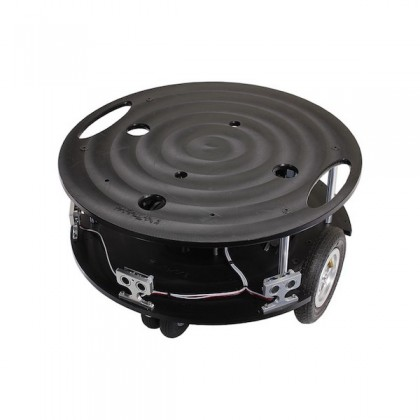
\includegraphics[width=.7\textwidth]{arlo real}
	
	\caption{Mobile robot Parallax Arlo \cite{arloreal}}
	\label{arlore}
\end{figure}


Equally to the Carolo-Cup regulations the lane width is defined by double robot width and therefore 900 mm. 

The robot is equipped with the following sensors:

\begin{itemize}
	\item Lidar
	\item Wheel encoder
	\item IMU
	\item Camera
\end{itemize}

Additional it features a motor driver for differential drive steering.

\section{Software}
Generally the software is developed for ROS-Noetic.\\
The programming language is mostly C++ to allow uniformity in the software stack.\\
Like in the Carolo-Cup the software is not supposed to have any connection to systems outside of the robot.\\

\subsection{Simulation}
Since the environment is simulated the simulator has to have the following features.
\begin{itemize}
	\item Sensor plugins with configurable error and ROS interfaces
	\item Differential drive plugin
	\item Custom models integration
	\item URDF conversion
	\item Not too computationally heavy
\end{itemize}

The simulation is mostly focus on sensor data. That is why sensor plugins with configurable error and a ROS interfaces are needed. Like this the data will be as representative as possible of the real world.\\

In addition to the sensor plugins the simulator needs to provide a plugin for differential drive steering. This is the replacement for the motor controller of the real robot.\\

Custom models is a strict requirement since this thesis focuses on a very specific robot. Furthermore the integration of custom models is necessary to put the robot in different road scenarios.\\

A URDF conversion plugin is very important like this differences between the simulated robot and the tf-tree in ROS can be avoided and the robot will be defined in one file only.\\

To get the best correlation between simulation and real world, the simulator should be able to run close to real time. This will make the simulated sensor data way more reliable and puts the nodes of the navigation\_stack under a realistic load.

\subsection{Navigation}
The navigation is supposed to cover free driving without obstacles, as well as with static obstacles avoidance. It will not cover dynamic obstacles, road sign detection or driving situations like intersections and parking.\\

Development of an entire stack exceeds the content of this thesis, so an open source navigation project will be used which needs to satisfy the following requirements.

\begin{itemize}
	\item Sensor input.
	\item Goal pose input
	\item 2D mobile platform support usage of the conventional drive systems like ackermann and differential
	\item Path planning in respect to the robots kinematic and shape, as well as the environment detected by the sensors.
	\item Path planning and navigation in totally unknown environments
	\item Velocity output as linear and angular velocities
\end{itemize}

\todo{beschreibung}


\chapter{Theoretical Background}
\label{theoretical_background}
This chapter will cover the needed theoretical background about the Gazebo Simulation, the Sensor Plugins, ROS and all of the used ROS packages.

\section{ROS}
ROS (Robot Operating System) is an open Source project developed by the ``Open Source Robotics Foundation''. Like the name suggests it is an entire Operating System for Robots including Hardware abstraction, low-level device control, implementation of commonly used functionality, communication between processes and package management.\\
Furthermore it provides tools and libraries to write, build and run code across multiple computers\cite{rosintro}.\\
\subsection{Packages}
This is the main structure for software in ROS. A package can contain many different Nodes, libraries, service etc.. Furthermore it is the smallest possible Structure that can be build by ROS\cite{rosconcepts}.
\subsection{Nodes}
Nodes are processes that perform computation. Since ROS is very fine granular, a system, that controls an entire robot can contain many nodes that are connected using topics. A package can be written with the use of one of the client libraries roscpp or rospy\cite{rosconcepts}.
\subsection{Plugins}
\subsection{Topics and service}
All of the ROS Nodes are connected with a publisher/subscriber like structure. The topic is basically just a name for a certain message.\\

Not only one node but unlimited many nodes can publish and subscribe to one topic. This generally can be seen like a message bus with not limited connection permissions\cite{rosconcepts}.

Unfortunately the Topic system is not well fitted for request and answers between two nodes, therefore the service structure has been implemented.\\ 
A node might offers a service under a certain node and an other node can call that service. Services can have any in- and output that can be specified in a ``.srv'' file\cite{rosconcepts}.

\subsection{RVIZ}
rviz is a 3D visualization tool offered by default in ROS. It offers functionality to visualize sensor and further geometric data.\\
\subsection{REP}
REP's (short for ROS enhanced proposals) are guidelines made and maintained by the ros community. It is highly advisable to follow the guidelines as much as possible.

Complying to these guidelines allows external people easier comprehension of the structure of the robot and eliminates misunderstandings.

The most important REP's in this project are REP 103 and REP 105.
\subsubsection{REP 103}
	
	"This REP provides a reference for the units and coordinate conventions used within ROS"\cite{REP103}\\  
	
	\textbf{Coordinate Frame}
	\begin{itemize}
		\item \textbf{X-Axis} - Forward
		\item \textbf{Y-Axis} - Left
		\item \textbf{Z-Axis} - Up
	\end{itemize}
	
	\textbf{Units}\\
	Units will always be represented in SI Units and their derived units.\\
	
	\textbf{The order of preference for rotations}
	\begin{enumerate}
		\item Quaternion
		\item Rotation matrix
		\item fixed axis roll, pitch, yaw
		\item Euler angles
	\end{enumerate}
	\cite{REP103}
	
\subsubsection{REP 105}
	"This REP specifies naming conventions and semantic meaning for coordinate frames of mobile platforms used with ROS."\cite{REP105}\\
	
	REP103 Applies for all fixed coordinate frames.
	
	\textbf{Coordinate Frames}
	\begin{itemize}
		\item \textbf{base\_link} is a fixed frame on the robot base. It serves as the reference points for all of hardware mounted on the robot itself like sensors.
		\item \textbf{odom} is a world fixed frame that serves as the reference for the pose of the robot.\\ Since the pose of the robot will drift over time it wont serve as a good long term reference.\\In most cases the odom frame will be computed using localization sensors like wheel odometry, imu's, visual odometry, etc. which leads to a continuous frame.
		\item \textbf{map} is a world fixed coordinate frame that serves as the reference for the odometry frame. It is also the base for a map of the environment such as the ones provided by slam algorithms. The frame is time discrete since it is mostly computed by localization algorithms.
	\end{itemize}
	
	That tree can be extended by an earth frame that would be the reference for the localization of the map in the earth. Which is useful, for long range robot platforms.\cite{REP105}
	
	
	
\subsection{TF}
In most cases robots that are controlled by ros have a so called tf\_tree. This tree is the coordinate frame structure of the robot. In it every sensor and actor has its own coordinate frame.\\
 The structure in most trees of mobile platforms is quite similar which is caused by the REP105 (ROS Enhanced Proposals) this contains a definition of recommended names for the robot frames and their order in the tree. But it should be noted that not every frame that is defined in the norm has to be in every tree. The basic structure mostly starts at a so called fixed frame. This Frame will be the not changing frame in the environment. At moving robots this is often earth, map or odom, while in stationary robots this can even be base\_link.\\
 

The tree is normally build up like in the following image. 

TF2 is the successor of TF and is a very powerful tool in the ROS environment. With it it is possible to transform sensor\_msgs and geometry\_msgs from one frame in another. Furthermore it offers the possibility to transform old data into the present or at any other point in the past.

\subsubsection{URDF and xacro}
The robot hardware description consists of one or more URDF(Unified Robot Description Format) based xml file. Its purpose is to define the shape and geometric of every part of the robot. 

\subsubsection{robot\_state\_publisher}
	This package uses the robot hardware description and builds up the tf\_tree using static\_transform\_publishers.

\section{Gazebo}


\subsection{Plugins}
Gazebo offers a wide selection of pre made plugins that can be incorporated into a simulated robot by attaching the plugin to the right tf\_frame and configuring its parameters.

\subsection{Models}


\section{navigation stack}
\subsection{move\_base}
\subsection{global\_planner}
\subsubsection{base\_global\_planner}
This is the default global planner of move\_base .
\subsection{local\_planner}
\subsubsection{teb\_local\_planner}

\subsubsection{dwa\_local\_planner}
\subsection{costmap}
A costmap is a grid stile map, whose purpose is to store information about obstacles in the surrounding of the robot.\\
There are two different costmaps, the global costmap and the local costmap.
The global costmap is by the global planner to find a collision free path. Whereas the local costmap is used by the local planner for local planning.\cite{navsetup}\\
\begin{figure}[H]
	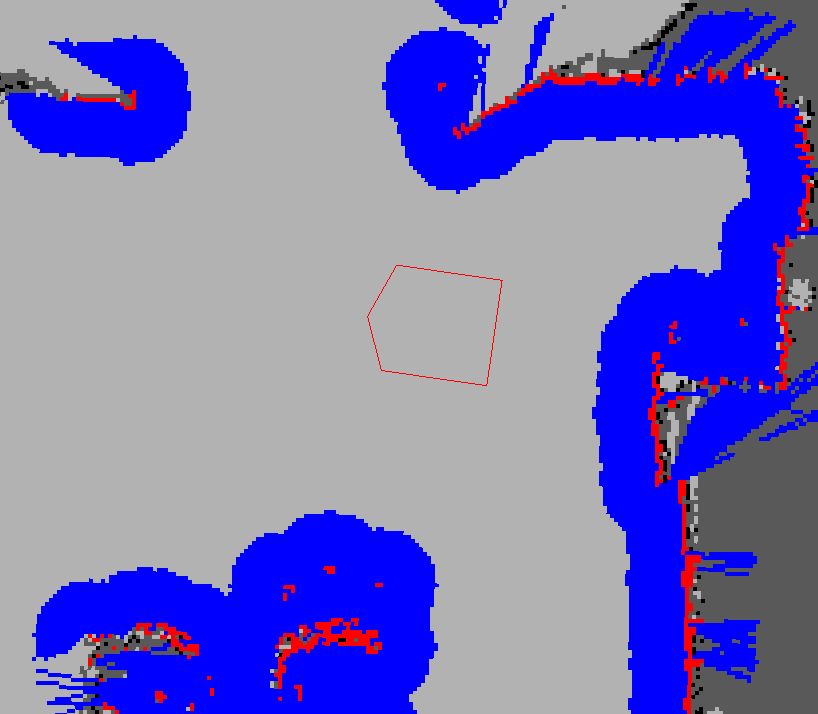
\includegraphics[width=\textwidth]{Pictures/costmap_rviz}
	\caption{costmap with obstacles and inflation \cite{costmap}}
	\label{costmap}
\end{figure}


\subsubsection{Cost Values}
The values in a costmap can be in the range [0-255], but the underlying structure categorizes them in the following 3 sections:
\begin{itemize}
	\item lethal obstacle
	\item free space
	\item no information
\end{itemize}

\subsection{marking and clearing}
Obstacles in the costmap can not only be marked, but also cleared by the subscribed data source. For each data source a configuration regarding the clearing and marking permissions is necessary. For clearing the costmap uses a raytracing algorithm, which allows the costmap to handle moving obstacles\cite{costmap}.
\subsubsection{Inflation}
Inflation is a process where a occupied cell is inflated by over the distance decreasing cost values for a configurable radius, as pictured in Figure \ref{costmap}.\\
This process is used by the default plugin inflation\_layer with the cost distribution pictured in Figure \ref{costdistribution}\cite{costmap}.

\begin{figure}[H]
	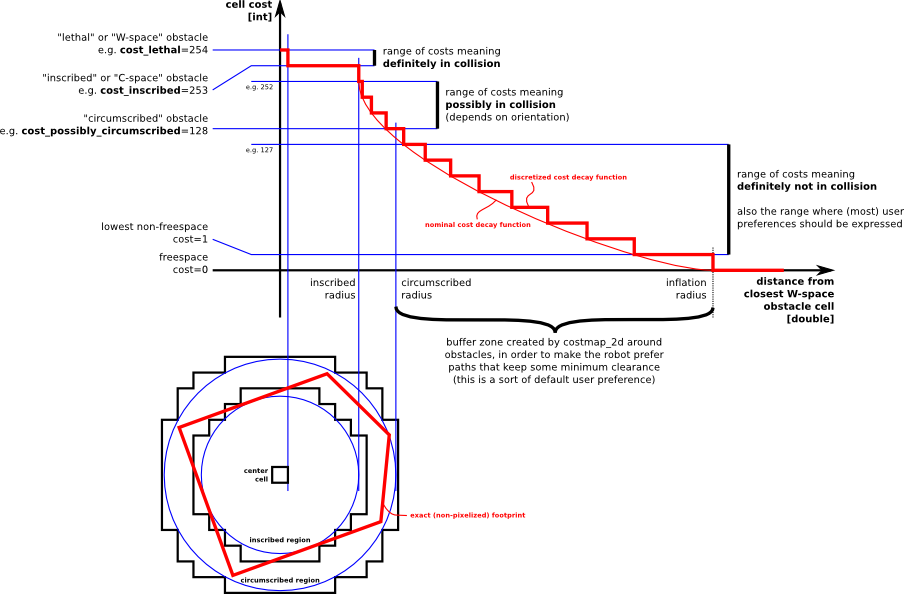
\includegraphics[width=\linewidth]{Pictures/costmapinflation}
	\caption{cost distribution and classification \cite{costmap}}
	\label{costdistribution}
\end{figure}

The usage of inflation has two reasons. First it is used to close gaps between two measured obstacles and therefore usefull, if the sensor resolution is relatively corse.\\
The second reason is to prevent the planner from getting too close to obstacles. Therefore the inflation radius is typically set to slightly more than the radius of the robot\cite{costmap}.

\subsubsection{layer}
The costmap uses a layer structure of plugins that can handle different tasks. The costmap then combines the data from each layer, to produce the final costmap.\\

By default the costmap\_2d package offers the following 3 layers:
\begin{itemize}
	\item \textbf{static map layer} is a layer that converts a prerecorded map into obstacles.
	\item  \textbf{obstacle layer} is a plugin that handles input from sensor sources. The plugin marks and raytraces obstacles in 2D. It can handle LaserScans PointCloud and PointCloud2.
	\item \textbf{inflation layer} handles the inflation of lethal obstacles in the costmap.
\end{itemize}

Furthermore the plugins Social ``Costmap Layer'' and ``Range Sensor Layer'' are offered.

Using the pluginlib interface and the costmap libraries one can develop custom layers for the costmap to achieve special behaviour of the robot.



\section{cartographer}
Cartographer is a Lidar based SLAM developed by Google. In contrast to gmapping it is based on loop closure to ensure real time mapping even in relatively big environments.\\
Submaps are considered for loop closure, if they are close to each other. A scan matcher tries to find constraints between the submaps and the current scan. When searching for loop closure constraints at a certain rate one can achieve basically instantaneous optimization of the map just by the fact that the current scan is similar to one of the underlying submaps\cite{cartographer}.\\

\section{Carolo-Cup}
The carolo cup is an event hosted by University Braunschweig and is an event in which the teams of many different universities can compete against each other and present their work and progress in the field of autonomous driving.

There are two different levels of difficulty the carolo basic cup and the carolo master cup.















\chapter{Related Work}
\label{relatedwork}

This chapter contains an analysis, of existing work in the field of ROS based robot navigation, especially with focus on a road like environment. The result of this analysis, can be used to outline the work that is necessary to satisfy the scope of this thesis.
\section{Path Planning}
Regarding the planning of the robot motion the GitHub Project ``ROS Planning'' provides basic implementations for motion planning and navigation\cite{rosplanning}.

This project includes the software stacks MoveIt!, navigation and navigation2, which are all implementations for the manipulation of robots.\\
\subsection{MoveIt!}
MoveIt! is the most widely used software for manipulation of robots. It is released under the Terms of the BSD license, which means it can freely be used in commercial, industrial and research\cite{moveit}.\\
It incorporates the latest advances in motion planning, manipulation, 3D perception, kinematics and navigation.\\

The software is an evolution of the arm\_navigation ROS packages that are designed for the manipulation of robot arms mounted on the PR2 robot from Willow Garage\cite{chitta2012moveit}\cite{willow}.

The evolution of arm\_navigation was an effort to separate the software from ROS, since a large part of ROS is not needed for the movement of the robot. 

Using URDF makes MoveIt! highly flexible to robot configurations, but the manipulation of ``arm-like'' robots is still one of the core tasks of the software.

\subsection{navigation}
In contrast to MoveIt! the navigation project of ROS-Planning is a software stack, that is developed to move a robot from Point A to Point B.

At first this seems like a fairly simple concept. The navigation takes in a goal, as well as odometry data in combination with sensor streams, resulting in the output of the translational and rotational velocity of the robot.

Since the navigation stack is a very flexible approach regarding the robot setup, the configuration of the underlying nodes and the supply of the inputs can be quite complicated\cite{nav}.

As pictured in the recommended navigation stack setup in Figure \ref{navigation stack setup}, it relies highly on the action move\_base, which has the general task of producing velocities based on the given goal.

\begin{figure}[H]
	\centering
	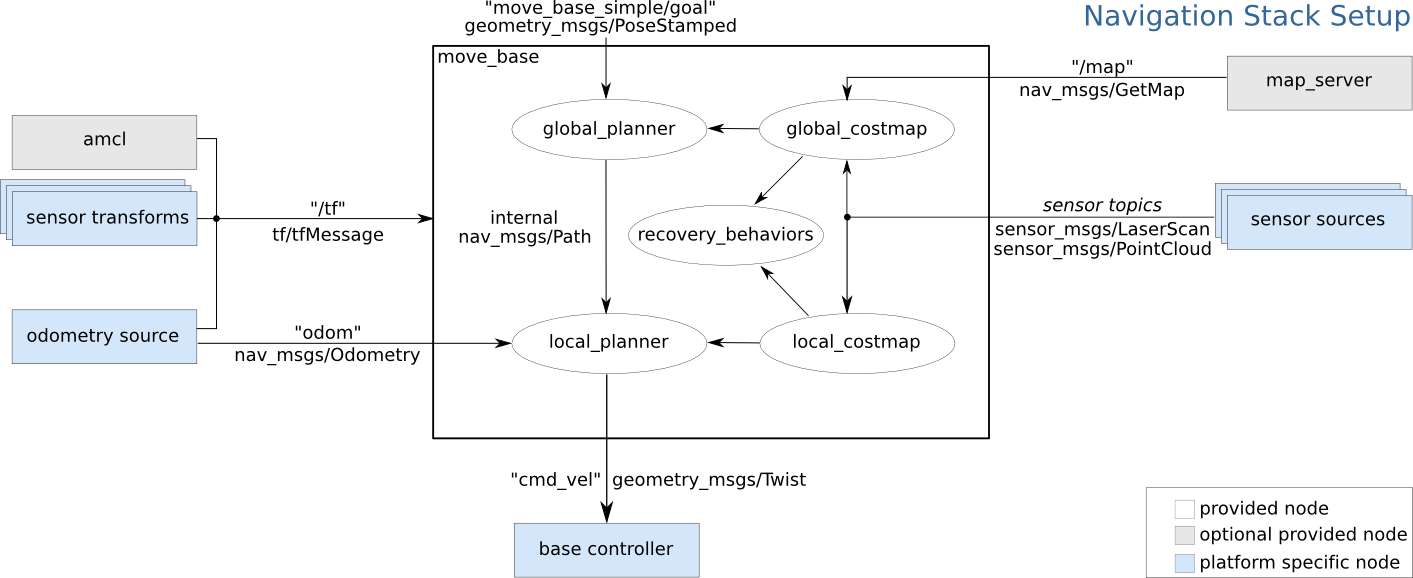
\includegraphics[width=\textwidth]{Pictures/navigation stack setup}
	\caption{recommended navigation stack setup\cite{movebase}}
	
	\label{navigation stack setup}
\end{figure}

The navigation stack has the option to navigate in an existing map by using the combination of the map\_server and amcl (adaptive monte carlo localization). The map\_server publishes a pre recorded map as an occupancy grid. The amcl package then uses that map for localization of the robot by matching the incoming scan result to the map published by the map server. With a good and detail rich map this allows for a accurate estimate of the robots position.\\

For the navigation of a robot the blue squares in the setup need to be supplied, as well as a source for the next goal. In addition every provided node needs to be configured according to the wanted behavior and the mechanical properties of the robot.\\

move\_base has been build very flexible, since it relies on planner plugins and the costmap\_2d package developed by David V. Lu.

This costmap is build in layers, where every layer has a different task and/or inputs. These layers are then combined into the ``master grid''. The master grid is the costmap layer used by the planners to calculate their paths\cite{costmappaper}. By adding additional layers, the navigation considers for example new sensor data or avoids certain sections of the robots environment.

Commonly used data is such produced by range finding sensors like lidar sensors or stereo cameras.\\

The layers provided in the costmap\_2d package are able to mark costs according to the range sensor data and an existing map. These cost can then be inflated by a fixed value radially\cite{costmap} to make an area around obstacles lethal.
\subsection{navigation2}

navigation2 is the successor of navigation, but is build for ROS2.
Since this thesis aims for a ROS-Noetic solution, the navigation2 stack will not be explored.

\subsection{Planners}

A lot of work has been done regarding path finding. In the navigation\_stack this task has been split into two parts, the global and the local planner.

The global planner is supposed to find a rough path that does not collide with any lethal cells in the costmap. In case of the default package global\_planner of the navigation stack, this is either done using dijkstra or A* algorithms.\\

Since the global planner does not consider the robot directly, the local planner is supposed to find a path that is feasible for the dynamics and the steering type of the robot\cite{movebase}.\\



dwa\_local\_planner is according to Kaiyu Zheng the recommended choice for the local planner\cite{navtuningguide}. This planner uses a dynamic window approach, which means the limits of translational and rotational velocities of the robot create a space of feasible trajectories.\\ 
From these possible trajectories a configurable amount will be forward simulated over a given amount of time. These trajectories can be evaluated using configurable weights in combination with the local costmap and the global path.

The ``best'' trajectory is then chosen based on the evaluation. Since the trajectory consist of a combination from translational and rotational velocities, these can be used as the input for the motor controller\cite{dwaplanner}.\\

The planners of move\_base are implemented in the form of a plugin. Therefore, not only the planners of the navigation stack are available, but additional ones developed by the ROS community.\\

A popular choice is teb\_local\_planner, which uses the timed elastic band approach, introduced by Christoph Rösmann in his paper about ``Trajectory modification considering dynamic constraints of autonomous robots``.\\
This approach uses the global path as an elastic band, that is repelled by obstacles located next to it and contracted by internal forces like the time constrain.\\
This time constrain is the main difference to the classic elastic band that tries to find the shortest path. At first this seems to be equivalent, since the shortest path should be the fastest but this does not consider the dynamics of the robot itself. 
The dynamics of the robot might prevent it from following the shortest path\cite{Rsmann2012TrajectoryMC}. 

This approach has been implemented in a way, that allows tuning of the individual weights for the deforming forces.\\

The consideration of thy dynamics lets the planner find the ``best'' combination of translational and rotational velocities to send to the motor controller.


\section{ArloBot}
ArloBot is a project of Christen Lofland regarding a Parallax Arlo platform. It consists of a set of ROS packages that allow the robot to navigate and generate a map of a room\cite{chrisl8}.

The navigation of this robot platform is controlled via a web interface, that allows the user to place goals for the robot to drive to, using the navigation stack.

\section{Work of other Carolo-Cup Teams}
In the field of autonomous navigation, a lot of work has been done by all teams that compete in the Carolo-Cup.\\

Unfortunately, there are only very few publications about the navigation software of other teams. Among these publications even less are ROS based and none is using a software stack proposed in ROS Planning.


\section{Summary}
The analysis suggest, that the navigation stack is a reasonable choice as a flexible base structure. MoveIt! is more distanced from ROS and rather focused on industrial arm-like robots. It does not seem to be fitting for the scope of this work.\\

Unfortunately, the navigation stack does not provide functionality to handle zones that are less preferred. This would be a useful feature to prioritize the right lane of the road. Therefore, modifications to the stack are necessary.\\


There has been a lot of research in path planning of robots. Even for different steering types. The presented solutions to these problems are not bound to a certain use case.
This thesis mainly focusses on the setup of a working navigation, therefore these planners can be used. The performance of these planners in a road environment are not tested yet but a selection procedure is needed. The development of custom planners for this use case might be necessary in the long term, if the performance is insufficient.\\

All of this covers only the navigation related nodes, but the navigation stack asks for inputs of certain types. The sensor setup is obviously specific to each robot platform. Additionally, to achieve the required navigation behavior, custom data filtering and processing is necessary.\\

As mentioned, work of other teams in the Carolo-Cup is rarely published and there are not yet any publications using the ros navigation stack. Furthermore it would defeat the purpose of the competition to take the concept of other teams as a reference.\\

While the project ArloBot of Christen Lofland does not share the same use case, it shares the same robot platform. The project is licensed under the definitions of the MIT License allowing unrestricted usage to any person. Therefore, the URDF file of the robot is already existent and will be used as a starting point in this project, although it might need modifications.















\chapter{Concept}
\label{Concept}

This chapter covers the conceptual design of the navigation and defines requirements for some of its parts.\\

Based on the analysis in chapter \ref{relatedwork} the navigation stack seems to be a well fitting core structure for the navigation. The use case leads to modifications to the recommended setup, pictured in figure \ref{navigation stack setup}.

Afterwards the tasks of the nodes in move\_base need to be defined. These will be categorized into the global and local stage, each consisting of a planner and a costmap.
Additionally the setup requires nodes, which autonomously find new goals for the navigation and transform the sensor data into a usable format. 

\section{Sensor Transforms}
To know the position of every sensor relative to the robot and its odometry the tf\_tree has to be build. While this can be realized by calculating the transformations between the frames manually,  using the ROS package robot\_state\_publisher is a cleaner approach. This requires a robot description in URDF format that specifies the relations between everything mounted on the robot.\\

The required transform from the base to the odom frame is build by using the position derived from the wheel encoder data.

\section{Map}

The map is a representation of the robots environment. With it go and no-go zones can be determined.\\

Unfortunately, amcl and the map\_server are not suited for this use case, since they require a prerecorded map of the environment. 

A SLAM (simultaneous localization and mapping) algorithm becomes highly useful since the robot might drive multiple rounds, allowing it to build its own map.\\
This potentially allows a goal extraction from the map instead of estimating it by using the sensor data stream. Furthermore it can be used to determine the robots position relative to the map, by providing a transformation between the map and odom tf frames.

Unfortunately, the data that can be fed to the SLAM algorithm is very limited, since it is not guaranteed, that the lidar sensor all ways sees static obstacles. Another data source for the SLAM algorithm could be the points extracted from the road detection. Unfortunately, the road markings are similar to a corridor and do not have a lot of features, other than their curvature.\\

This significantly decreases the reliability of the map which therefore will highly depend on good odometry, since for example a straight section of the road always looks similar, even if it is on the other side of the circuit. The odometry provides an estimate, where the SLAM algorithm should attach the sensor data to the map.

To get a better map, both of the data inputs have to be used, which results in the need of a SLAM algorithm with multiple inputs.\\

\section{move\_base}

move\_base consist of a global and a local part, the combination of both defines the path finding characteristic of the navigation. Since each part has a different task they can be separated into the global and local stage.

\subsection{Global Stage}
The general task of the global planner is like described in the theoretical background to plan a rough path through the grid of the costmap, that does not collide with any lethal cell.\\

In this scenario the global planner will also be used to guide the robot on the correct lane. This results in the following requirements:

\begin{itemize}
	\item The global costmap needs information about the road markings and the obstacles detected by the lidar scan
	\item The global costmap needs to incorporate cost that generate a preference for the right lane, but allow the global path to go to the left lane in case of an obstacle
	\item The global planner has to respect all cost values
\end{itemize}

\subsection{Local Stage}
The local stage on the other hand has the task of finding a path, that is feasible for the dynamics of the robot and does not collide with objects.\\
This path is supposed to be close to the global path and follow its lane changes, but it needs to be able to separate itself from it, if necessary.

Therefore the local costmap needs to contain information about the road markings and the obstacles detected by the lidar scan.

\section{PoseFinder}
The job of this node is to extract a goal from the sensor data or the map.\\

The road detection is only able to detect the road to a certain distance. Everything beyond is unknown.\\
To allow the planners to generate smooth paths the distance, at which goals need to be found should be relatively far away from the robot. Therefore this node needs to estimate the upcoming course and repeatably send new goals. Since this approach uses estimations, it is uncertain if the goal is actually on the road or not.

If a map is available the estimation is redundant, since the map is likely to be more precise.

\section{Sensor Filter}

This block incorporates the nodes that process the sensor data into a format, that is usable for the navigation\_stack. 
Therefore it consists out of the following nodes:

\begin{itemize}
	\item \textbf{roadDetection} will extract approximated polynomials for the road markings and the lanes from the camera data
	\item \textbf{markfreespace} needs to publish point clouds to the costmaps and the SLAM algorithm consisting of the road detection data and the lidar scan.
\end{itemize}

Like described in the requirements, the simulator is supposed to produce realistic sensor data, which might need filtering. These filters are additionally located in this block.

\section{Resulting Concept}
The schematic in figure \ref{navconcept} shows the concept of the navigation.  To keep the schematic as simple as possible, not every connections between the nodes are highlighted (Appendix \ref{config} shows the finalized schematic).\\

\begin{figure}[H]
	\begin{center}
		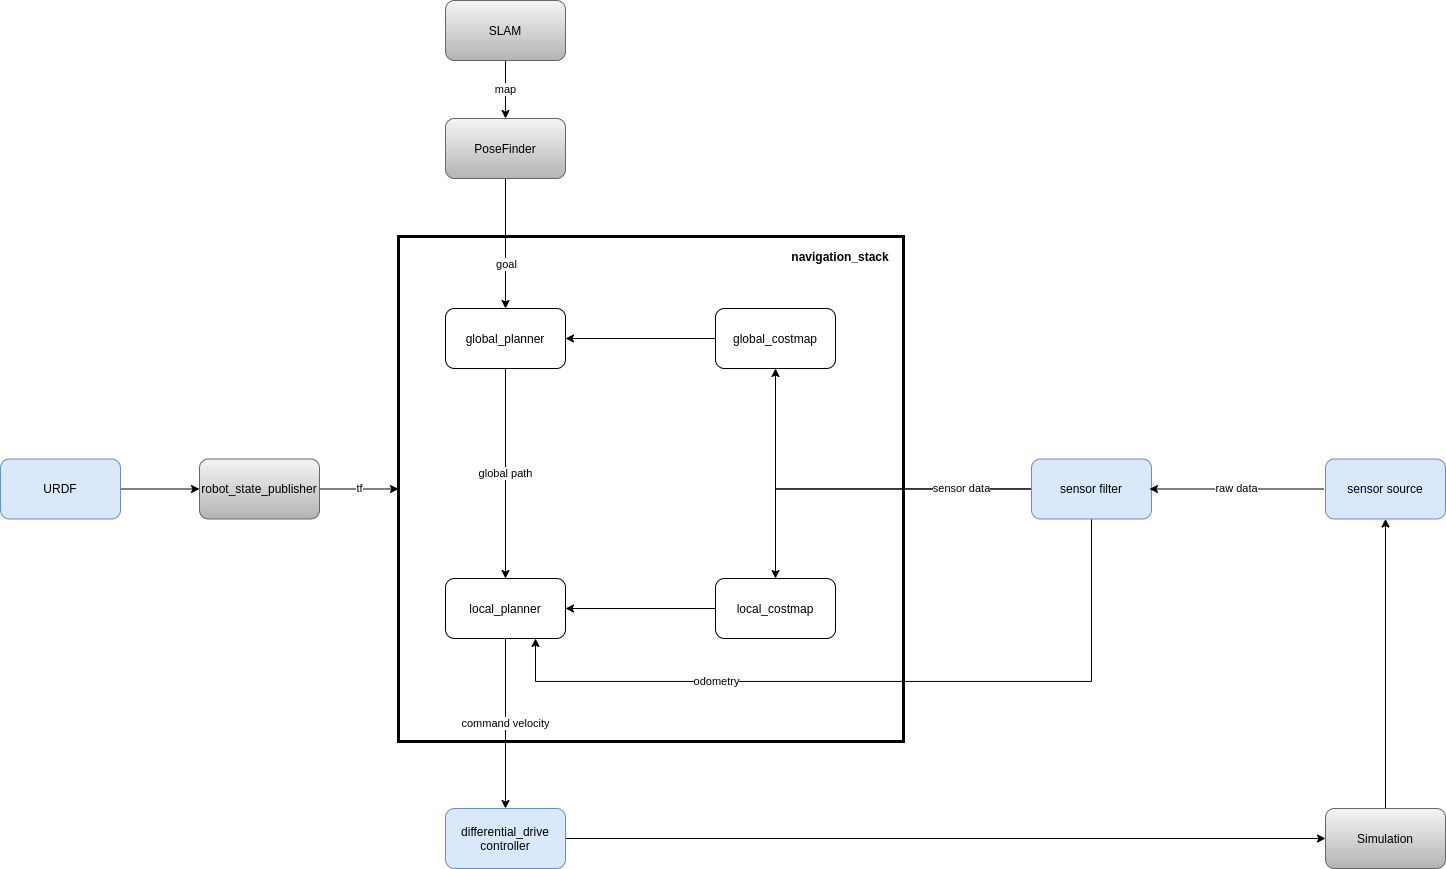
\includegraphics[width=140mm]{Pictures/Updated navigation concept}
		\caption[updated navigation concept]{Updated navigation concept (Blue - platform specific nodes, Grey - optional nodes, White - move\_base nodes)}
		\label{navconcept}
	\end{center}
\end{figure}



The PoseFinder will repeatedly find goals based on the current state of the map and the sensor data. The goals will then be handed over to the navigation stack. This uses the filtered sensor data to determine, where the robot is as well as, where it is allowed to go and where not. Afterwards the cascading planners produce first a rough, collision free, path on the correct lane and then a path that is possible for the dynamics of the robot. This path then gets converted to velocity commands and sent to the motor controller.\\






\chapter{Selection and development}
\label{Selection}

This chapter covers the package selection and the setup of all nodes in the concept. In addition to that the development of the custom nodes will be discussed. This results in nodes assigned to each block in the schematic pictured in Figure \ref{navconcept}.


\section{Simulation}
There are many options, when it comes to robot simulation environments, which makes a proper selection mandatory. The chosen simulator then needs to be configured and equipped with models, sensors and a drive system.

\subsection{Selection}
To begin of the selection process a group of reasonable simulators needs to be collected. The two selected options are Gazebo and V-REP since they are the two most used robotics 3D simulators \cite{SimComp}.\\
The newest version of V-Rep is now called CoppeliaSim. Unfortunately, there are no comparisons between it and Gazebo yet. Performing a thorough comparison between both would exceed the scope of this thesis. Therefore, its predecessor V-Rep will be compared. \\

Both simulators seem to fulfill most of the defined requirements to a certain extend, while Gazebo seems to have a easier installation process and integration into ROS.\\
Gazebo is included in the default packages of ROS Noetic since it is developed by the Open Source Robotics Foundation as the default simulator for ROS\cite{ROSPkg}.

V-REP, as well as Gazebo, offers plugins and URDF conversion for custom models, but an even bigger selection of mobile robot models. Unfortunately, they can only be used as examples since the required models are very specific.\\
In contrast to V-REP, Gazebo does not contain an integrated model editor.

The comparison in the paper of L. Pitonakova et al. regarding computational load shows, that V-Rep is the most resource hungry environment, when compared to  Gazebo\cite{Pitonakova}. Real time simulation is highly wanted in this thesis, so the results can be compared to real results in the future.

Based on the fact, that Gazebo is included in the ROS-Noetic package list and has a smaller computational load compared to V-Rep, it will be the simulation environment in this project.

\subsection{Model}
Since Gazebo doesn't have an integrated model editor the freeware ``Blender'' will be used for the generation of the model of the environment, since it has options for exporting COLLADA files (.dae) usable in Gazebo.

As described in the requirements the robot models will be generated using URDF which will be covered later.

\section{move\_base}

As described in the concept, the navigation stack will be used in this thesis. Therefore, the action move\_base will be used to get the robot to a given goal.\\
 move\_base incorporates nav\_core and costmap\_2d and their internal nodes, which need to be selected according to the requirements of the navigation.\\
Similar to the separation described in the concept (chapter \ref{concept})the nodes will be categorized into a global and local stage and discussed individually.

\subsection{Global stage}

\subsubsection{Planner}

Since the global planner needs to communicate with the nav\_core interface  the following selection as described in the documentation of nav\_core can be used as possible candidates\cite{navcore}:

\begin{itemize}
	\item global\_planner
	\item navfn
	\item carrot\_planner
\end{itemize}


Here the choice is fairly easy, since base\_global\_planner is the successor of navfn. It still supports the the behavior of navfn, but it offers more options, such as A* planning algorithm instead of Dijkstra.


carrot\_planner isn't suited for this use-case since it doesn't fullfil the requirement of being able to cover lane changes since it will not generate plans, that go around obstacles. Instead it will generate a straight path to the goal and shortens the path if the goal is behind or in an obstacle\cite{corrotplanner}.

\subsubsection{Costmap}
Since costmap\_2d is embedded in move\_base the package does not need to be selected itself. Instead the layers of the individual costmap need to be selected.\\

As defined in the concept, the global costmap needs to have information about lethal obstacles, road markings, as well as a defined preference for the right lane.\\


The data, supplied by the lidar and the road detection, can be marked as lethal obstacles in the costmap using the obstacle layer. This data consist solely from points, meaning there are gaps between the individual measurements. In the case of the lidar, these size of these gaps increase with the measurement distance.\\

As soon as these gaps are larger than the resolution of the costmap, free cells will start to appear between the measurements, that allow the planner to generate paths through obstacles or the road markings.\\

To solve this issue the default layer ``inflation\_layer'' can be used. This layer inflates every lethal cell in the costmap by a fixed radius, closing the previously discussed gaps like pictured in figure \ref{costinfl}.\\

\begin{figure}[H]
	\centering
	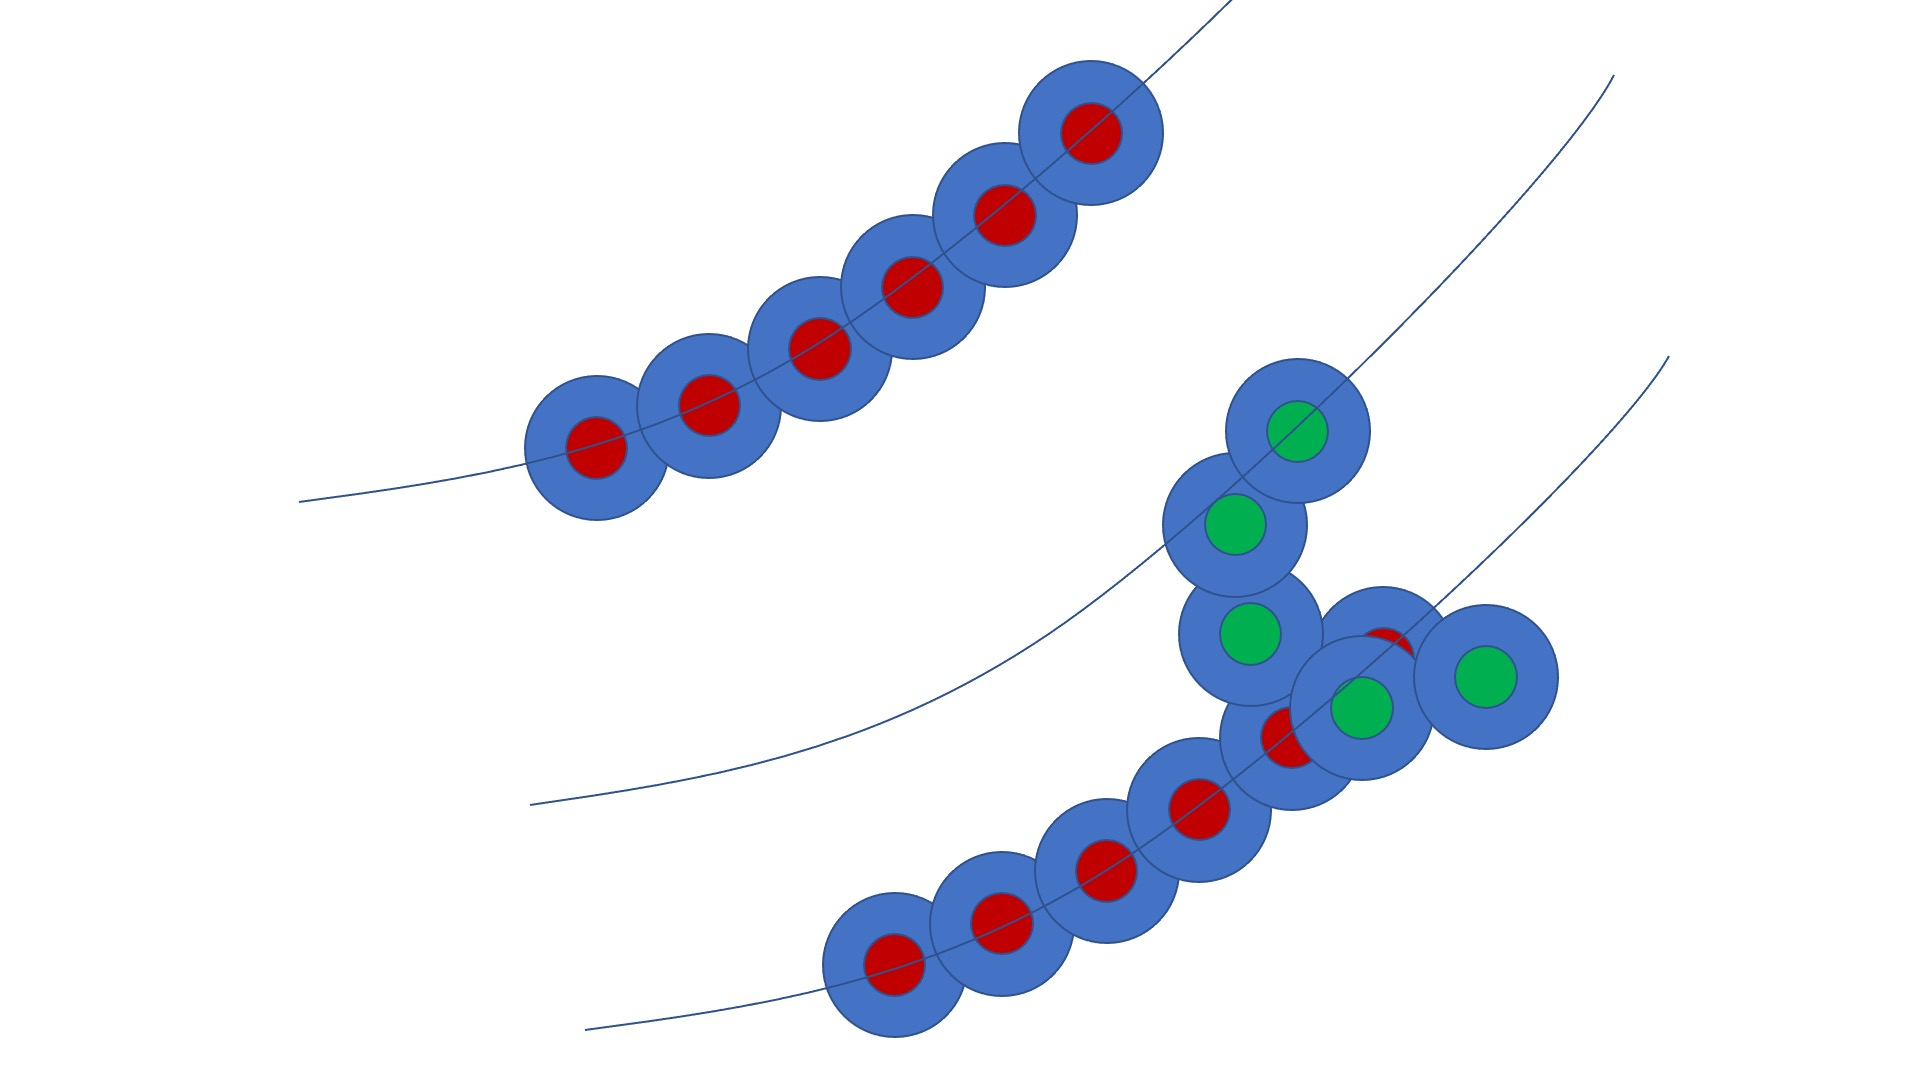
\includegraphics[width=.7\textwidth]{Pictures/costmap inflation}
	\caption{visualization of the inflated sensor data in the costmap (red - road detection, green - lidar scan, blue - inflation)}
	\label{costinfl}
\end{figure}

This configuration allows the navigation to plan around obstacles, without leaving the road, but there is no preference for the right lane yet. To generate this preference the left lane has to have higher cost than the right lane, without being lethal.

Unfortunately, this can not be solved using the provided layers. Therefore a custom layer has to be developed.

The only information about where the lane is, comes from the road detection, which outputs polynomials that approximate the road markings. The aim is to make a gradually increasing cost from the middle of the right lane to the left road marking. Therefore, the left road marking needs to be inflated using dynamically adjustable parameters for the cost distribution.\\


To guarantee, that driving on the right lane, the right road marking will be inflated, but with a different cost distribution. Here only the road marking is lethal, whereas the lane should be free resulting in the cross section pictured in \ref{globalcostdistro}. To simplify lane changes in the case of obstacle avoidance these obstacles need to have a cost free zone around them.\\

The layer should also feature a reset option as a recovery behavior.

\begin{figure}[H]
	\centering
	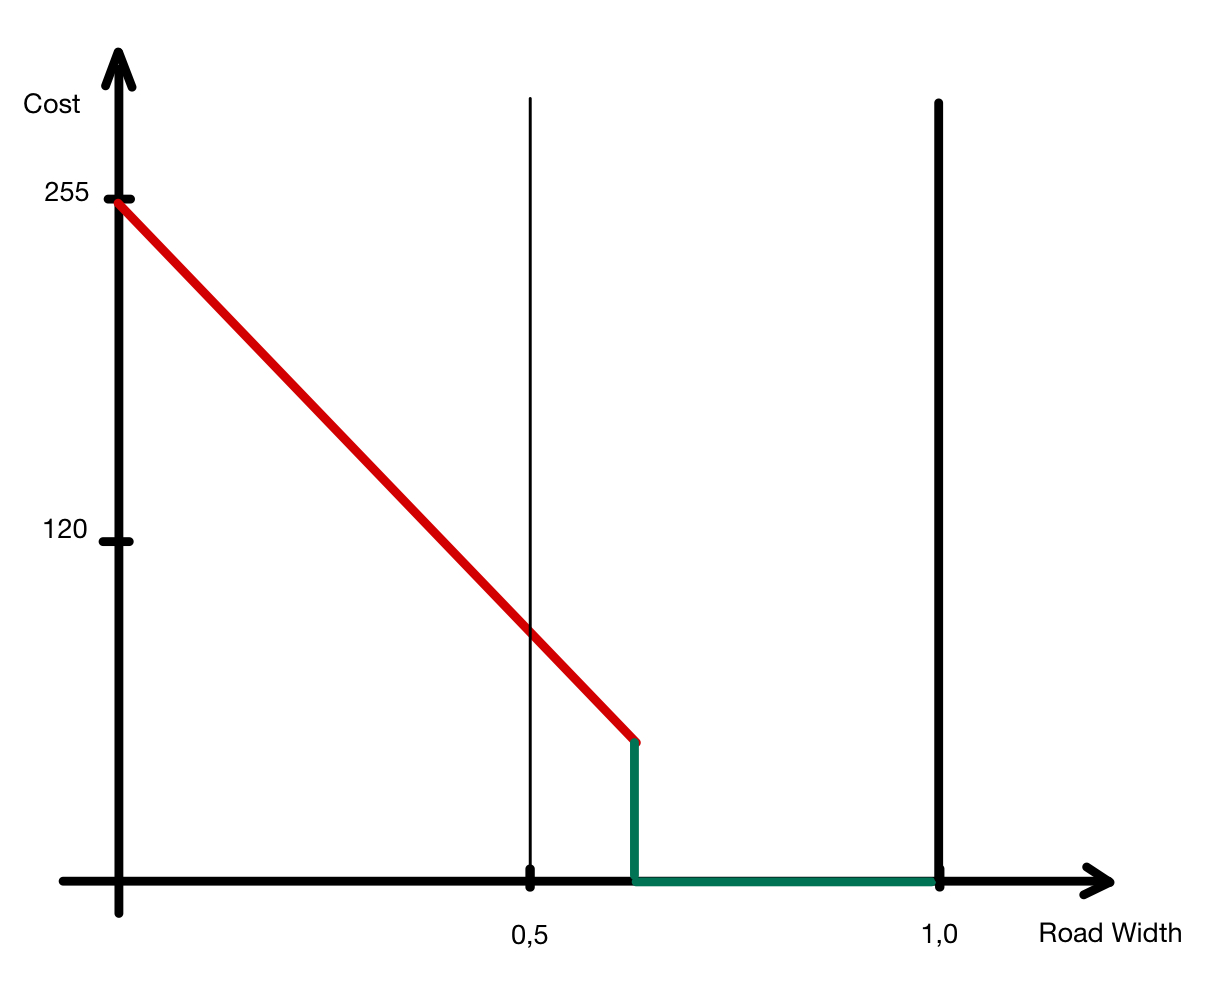
\includegraphics[width=.8\textwidth]{Pictures/global stage cost distro}
	\caption{global costmap cross section of the road}
	\label{globalcostdistro}
\end{figure}



The previously discussed tasks for the layer can be summarized in the following requirements:

\begin{itemize}
	\item Input for points
	\item Input of point individual inflation parameters
	\item Rasterization of the individual cost distribution
	\item Service to reset the cost in the layer
\end{itemize}



\subsection{Local stage}
\subsubsection{Planner}
In contrast to the global planner there are way more options for the local planner node to choose from. Like the global planners the local planners will be selected using the options offered in the following description of nav\_core\cite{navcore}.

\begin{itemize}
	\item base\_local\_planner
	\item dwa\_local\_planner
	\item eband\_local\_planner
	\item teb\_local\_planner
	\item mpc\_local\_planner
\end{itemize}

To choose the local planner the requirements have to be defined first.\\

Since the global planner is taking care of the obstacles and the road lanes, the local planner has the general task of following the global path and creating a command velocity that is feasible in regards to the dynamics of the robot.\\

Smooth lane changes are highly wanted in this project. This will help the camera and therefore the road detection to keep seeing the road during a lane swap. To achieve this, the planner is supposed to drive close to the global plan and to smooth out the edges.
Furthermore the local planner needs to have a good performance in tight corridor situations, since those will often be caused by obstacles blocking one lane.\\

During all of this the local planner needs to use the information of lethal obstacles to prevent crashes in its optimized path.\\


Base and DWA are two planners that are included in the navigation stack. Similar to the global planner selection, the successor and therefore DWA is chosen seems like a good option. According to Kaiyu Zeng, this is the general recommendation for mobile robotics platforms\cite{navtuningguide}. As described in the theoretical background, dwa struggles with navigation in narrow corridors and therefore can not be used.

In contrast to the method of the dwa planner, the elastic band approach is better suited for narrow corridors. The two planner, that use this approach are eband\_local\_planner and teb\_local\_planner. Choosing between these two is difficult, since they both share the same base principle. teb\_local\_planner is better suited for this use case, since it supports both car like and differential robots.

mpc\_local\_planner is build using the popular model predictive control approach. According to Christoph Rösmann (the developer of both planners), teb is preferred when dealing with simple differential or car like robots\cite{mpcvsteb}. 

According to the previous analysis teb\_local\_planner has the best fit to the use case and therefore selected for the navigation.


\subsubsection{Costmap}
The local planner is only supposed to generate velocity commands that lead to no lethal collision. Therefore, the local costmap will have the same layers as the global one without the dynamic inflation layer that is used to guide the robot to the right lane.


\section{PoseFinder}
As described in the concept the purpose of this node is to determine the pose of the next goal and send it to the move\_base action client. Therefore, it will need to process the data from the road detection and if available from the SLAM map to determine a feasible goal.\\

Since the robot should never reach a goal, the PoseFinder needs to determine new goals at a configurable frequency. 

\subsection{Usage of Current Camera Data}


The easiest way to get new goals, is to take the last point of the polynomial provided by the road detection as the position and calculate the yaw angle of the new goal with the gradient of the last two points.\\

While this is a logical approach in an ideal scenario, it certainly will not work in a realistic one, since a continuous data stream from the road detection can not be guaranteed, as shown in the edge cases pictured in figure \ref{nav edge case}.\\

In all examples pictured in figure \ref{nav edge case}, the road detection is not able to detect the road. If the robot would only follow the lanes detected by the road detection, it would not be able navigate in these situations, leading to stop of the robot.\\

This introduces the requirement for the PoseFinder, to find goals by estimating the course of the road, based on the latest data of the road detection. Therefore the navigation bridges the gap, in which the camera can not see the road.\\

\begin{figure}
	\centering
	\begin{subfigure}{.24\linewidth}
		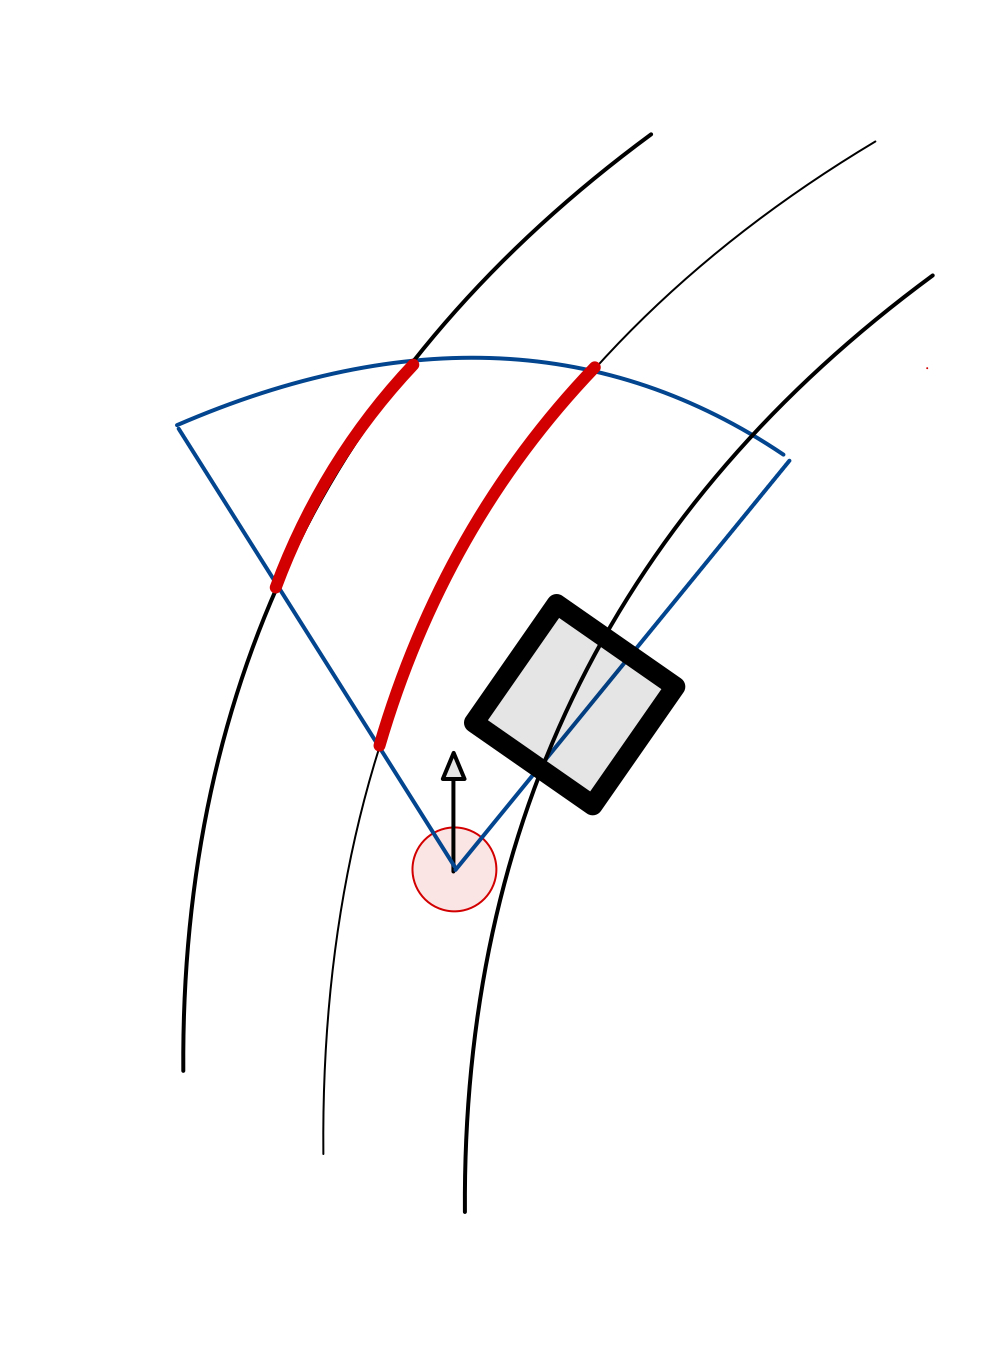
\includegraphics[width=\textwidth]{Pictures/road detection obstacle}
		
		\caption{lane markings blocked by obstacle}
	\end{subfigure}
	%\hskip2em
	\begin{subfigure}{.24\linewidth}
		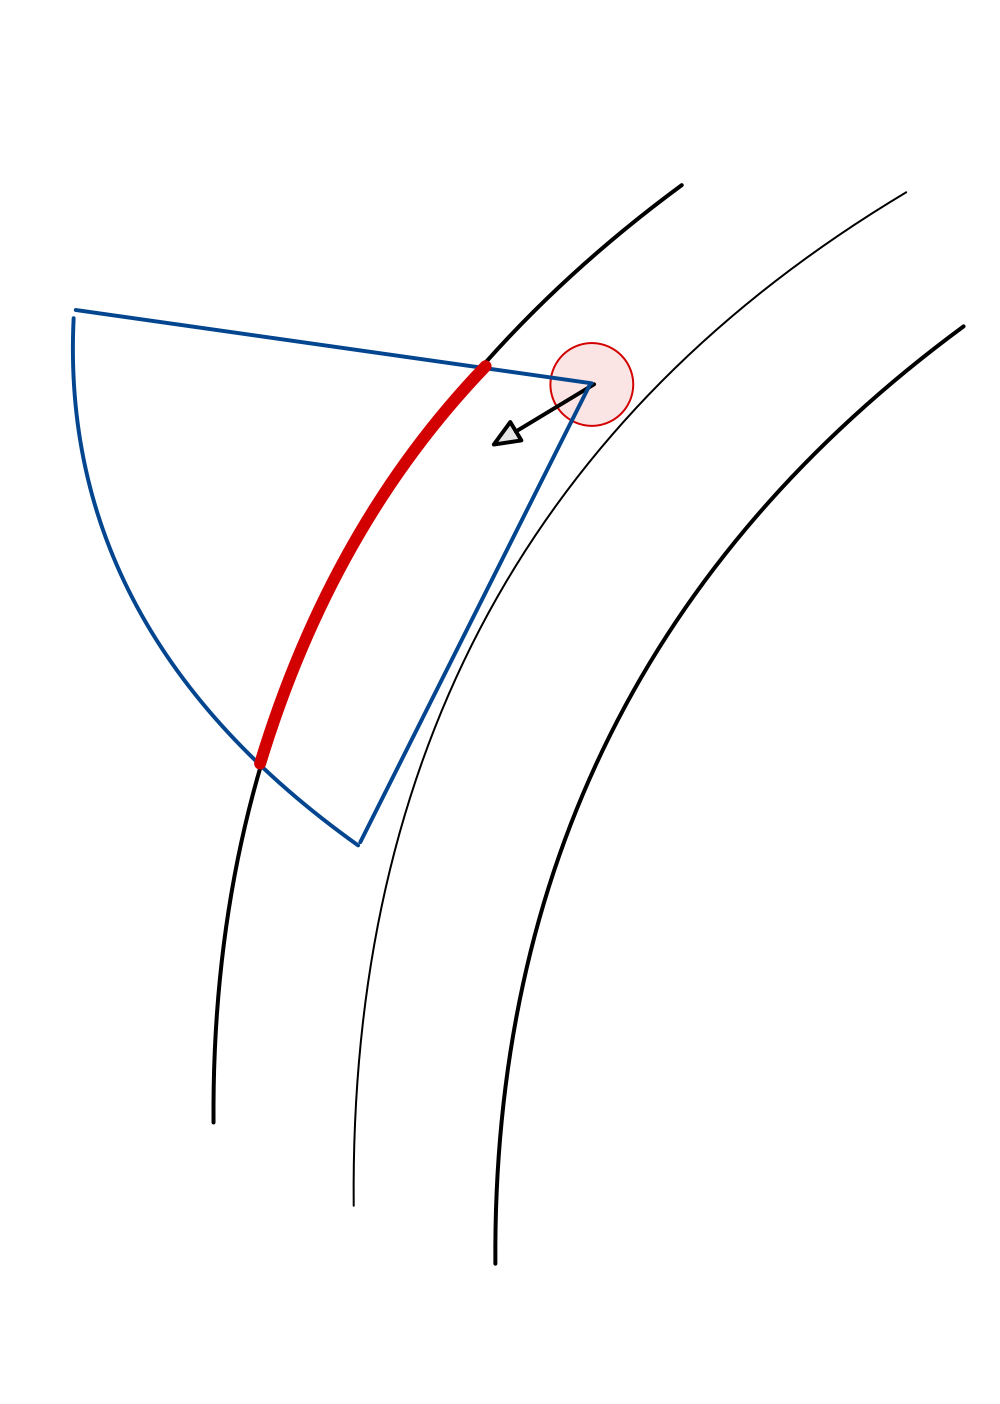
\includegraphics[width=\textwidth]{Pictures/road detection angle}
		\caption{driving in a corner}
	\end{subfigure}	
	%\hskip2em
	\begin{subfigure}{.24\linewidth}
		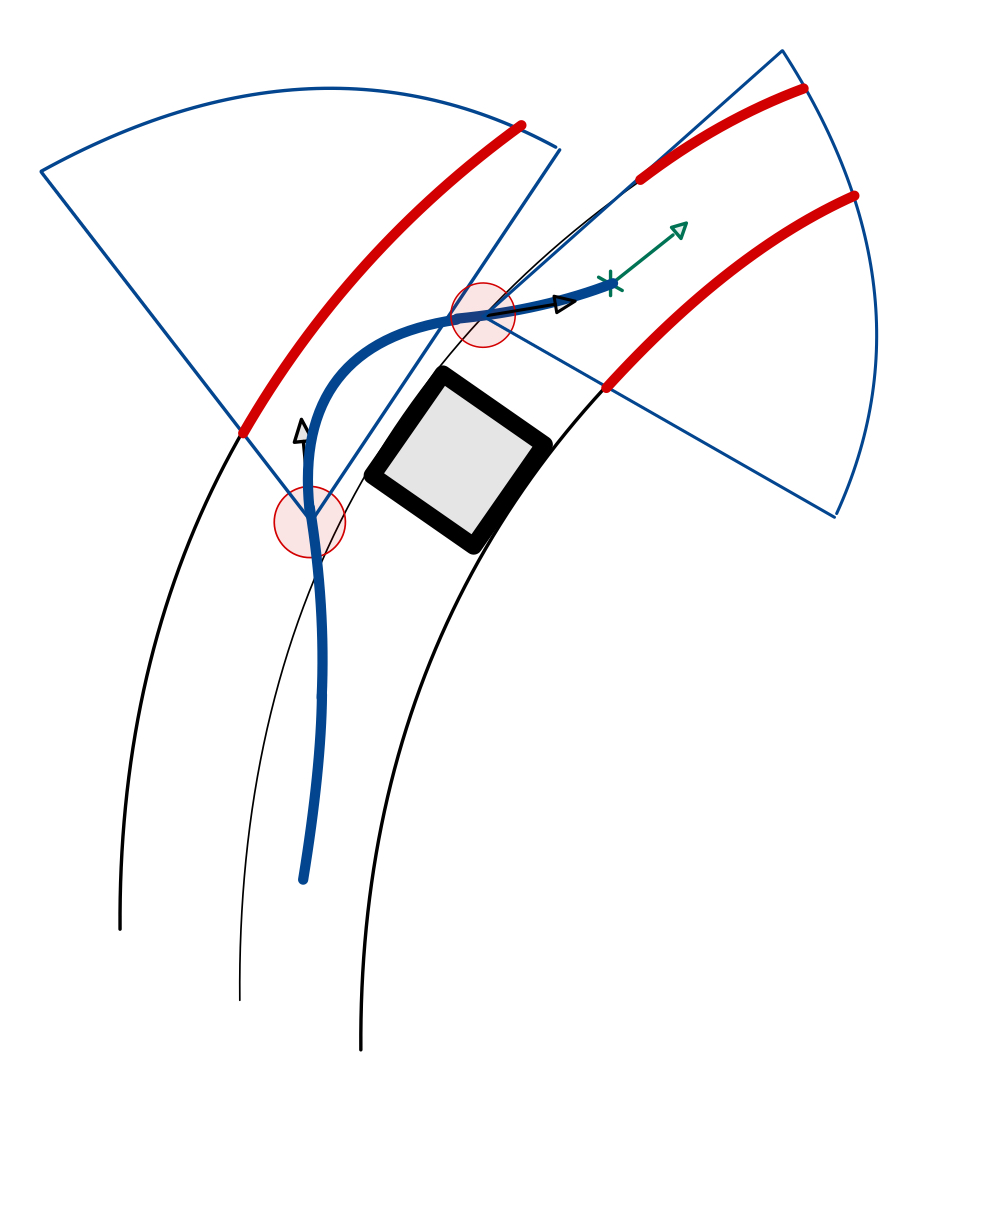
\includegraphics[width=\textwidth]{Pictures/road detection blind}
		\caption{camera angle during avoidance}
	\end{subfigure}
		%\hskip2em
	\begin{subfigure}{.24\linewidth}
		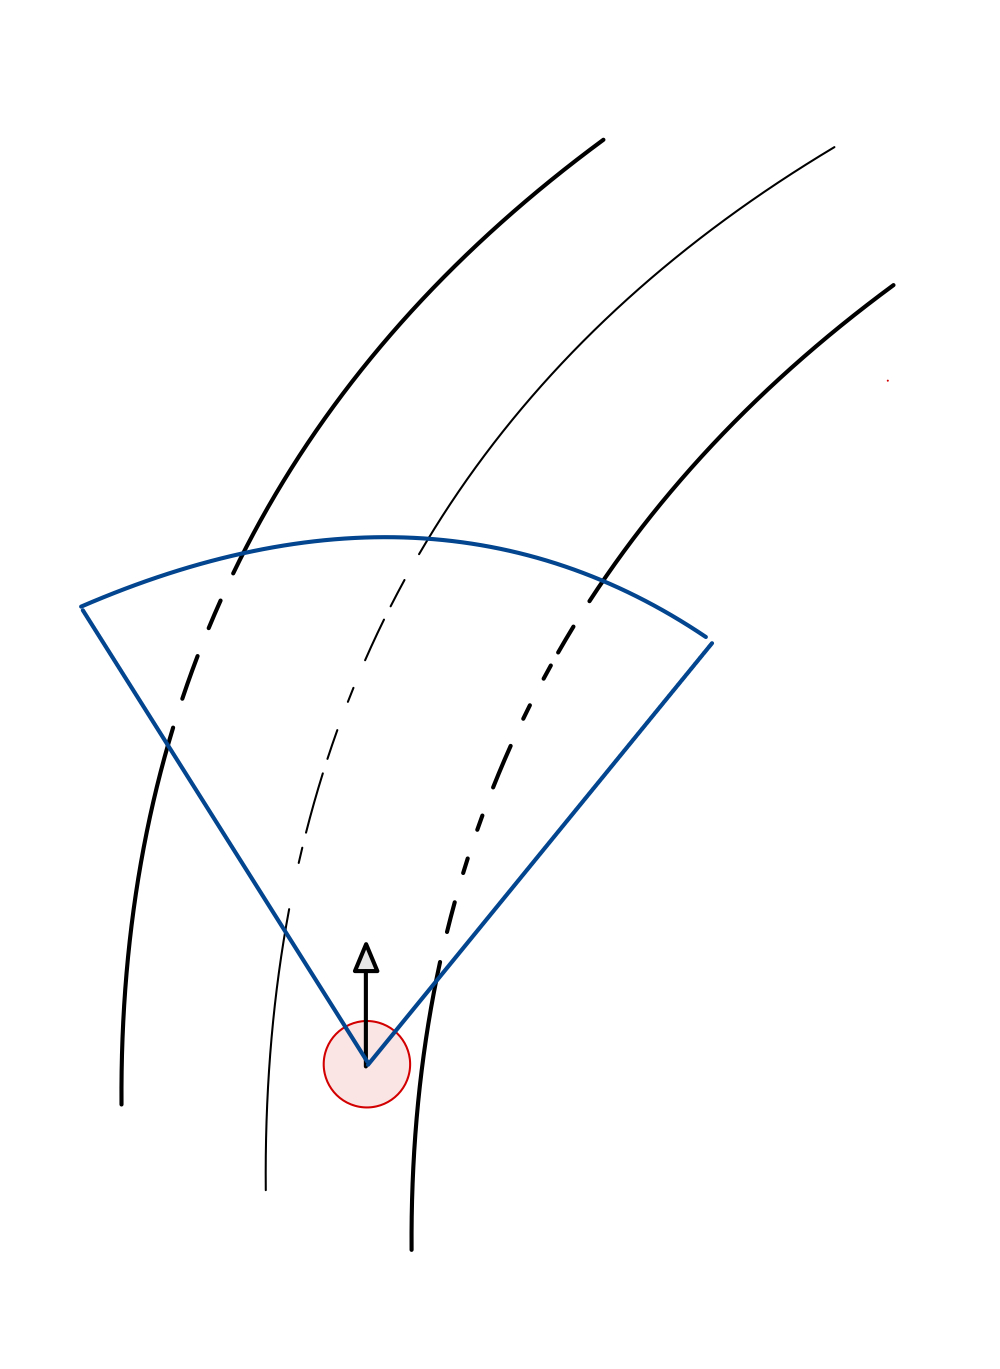
\includegraphics[width=\textwidth]{Pictures/road detection noise}
		
		\caption{camera noise or bad road markings}
	\end{subfigure}


	\caption{edge cases that prevent simple lane following}
	\label{nav edge case}
\end{figure}



\subsection{Approximations}
\label{aprox}
The approximation provided by the road detection is in the form of a polynomial. These describe the real road very accurately, but only in a very restricted domain. Outside of this domain, these polynomials diverge rapidly from the real road, making them unusable for any estmates.

Since the road mostly consists of circles of varying radii and origins, it is self evident, that using the polynomials in their restricted domain to represent a section of a circle will give a better estimate.\\
This circle can be calculated using the least square approach presented in Randy Bullocks paper on least square circle fitting \cite{leastsquarecircle}.\\

In theory this approximation should work for nearly straight sections as well. This will cause radius and origin to trend to infinity. Caused by camera noise and the inaccuracy of the road detection the representation of straight sections will get increasingly inaccurate.\\

Similar to the least square approach for circles, an approach for the lines can be formulated.

Switching between the result of the two approximations will produce the best result for both scenarios. This switching will be triggered by the radii of the approximated circles exceeding a configurable threshold.\\

The next step is a goal extraction from the chosen approximation. This goal will be calculated at a given distance from the robot origin on the approximated route. In contrast to the approximated lines, the circles have a defined angle of trustworthiness. Otherwise small circles would cause the goal to be way of the prediction. The orientation of the goal will then be determined using the derivative of either, the approximated circles or lines.\\

With the calculated points on both circles or on both lines the mean can be calculated and represents the new goal for the robot.

\begin{figure}[H]
	\centering
	\begin{subfigure}{.45\linewidth}
		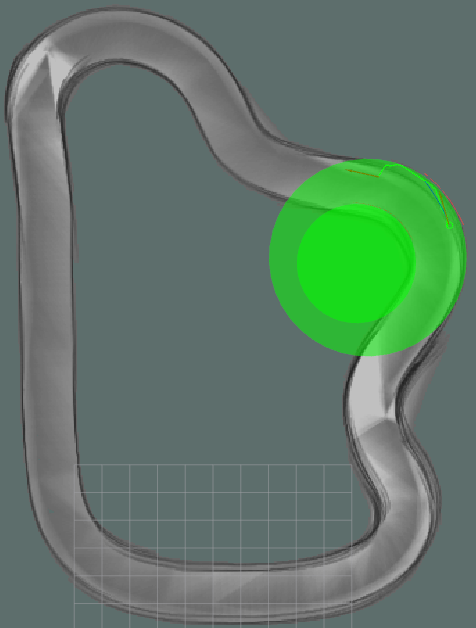
\includegraphics[width=\textwidth]{Pictures/circle approx}
		\caption{circle approximation}
		\end{subfigure}	
	%\hskip2em
	\begin{subfigure}{.45\linewidth}
		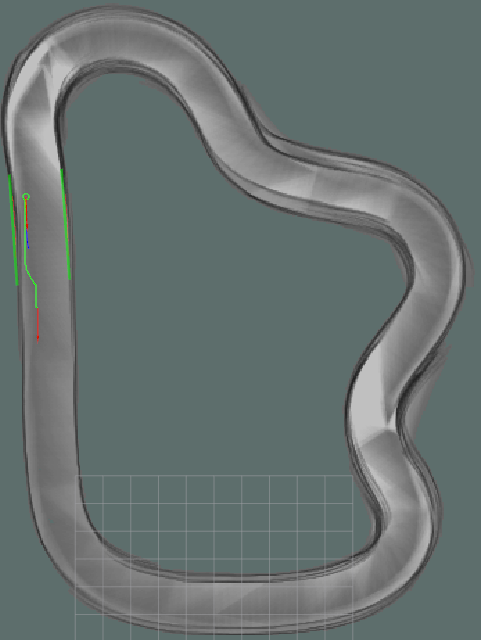
\includegraphics[width=\textwidth]{Pictures/lineapprox}
		\caption{line approximation}
	\end{subfigure}

	\caption{Approximations visualizations}
	\label{aproxvis}

\end{figure}

A visualization of the result is pictured in figure \ref{aproxvis}.
It shows the robot, its current goal, as well as the estimated road outlined by the geometric shapes of the respective approximation.

Based on this figure the necessity of the angle of trustworthiness of the road detection becomes apparent. Assuming a larger goal distance the estimated goal would not be located on the road anymore and would point in the wrong direction as well. This makes pathfinding impossible without leaving the road.


While these approximations allow the robot to bridge the edge cases pictured in \ref{nav edge case}, this approach introduces new problems. Since the goal is now determined by using estimations, it is uncertain if the goal is located off the road, or even in an obstacle. This problem is pictured in figure \ref{goaluncertainty}. Here the goal of the navigation is located within an obstacle. This would make path finding to the goal impossible.\\

To solve this issue the navigation has to consider obstacles, only if they are significantly closer to the robot than the goal. Therefore, the navigation treats the road as ``free'' until the obstacle is close to the robot. At this moment the predicted goal is way behind the obstacle, leading to an avoidance as described in the requirements of the navigation.

This does not only affect the distance, at which the PoseFinder estimates goals, but also the distance at which obstacles are treated as such and marked in the costmap, which has to be considered during the configuration.

\begin{figure}
\centering
	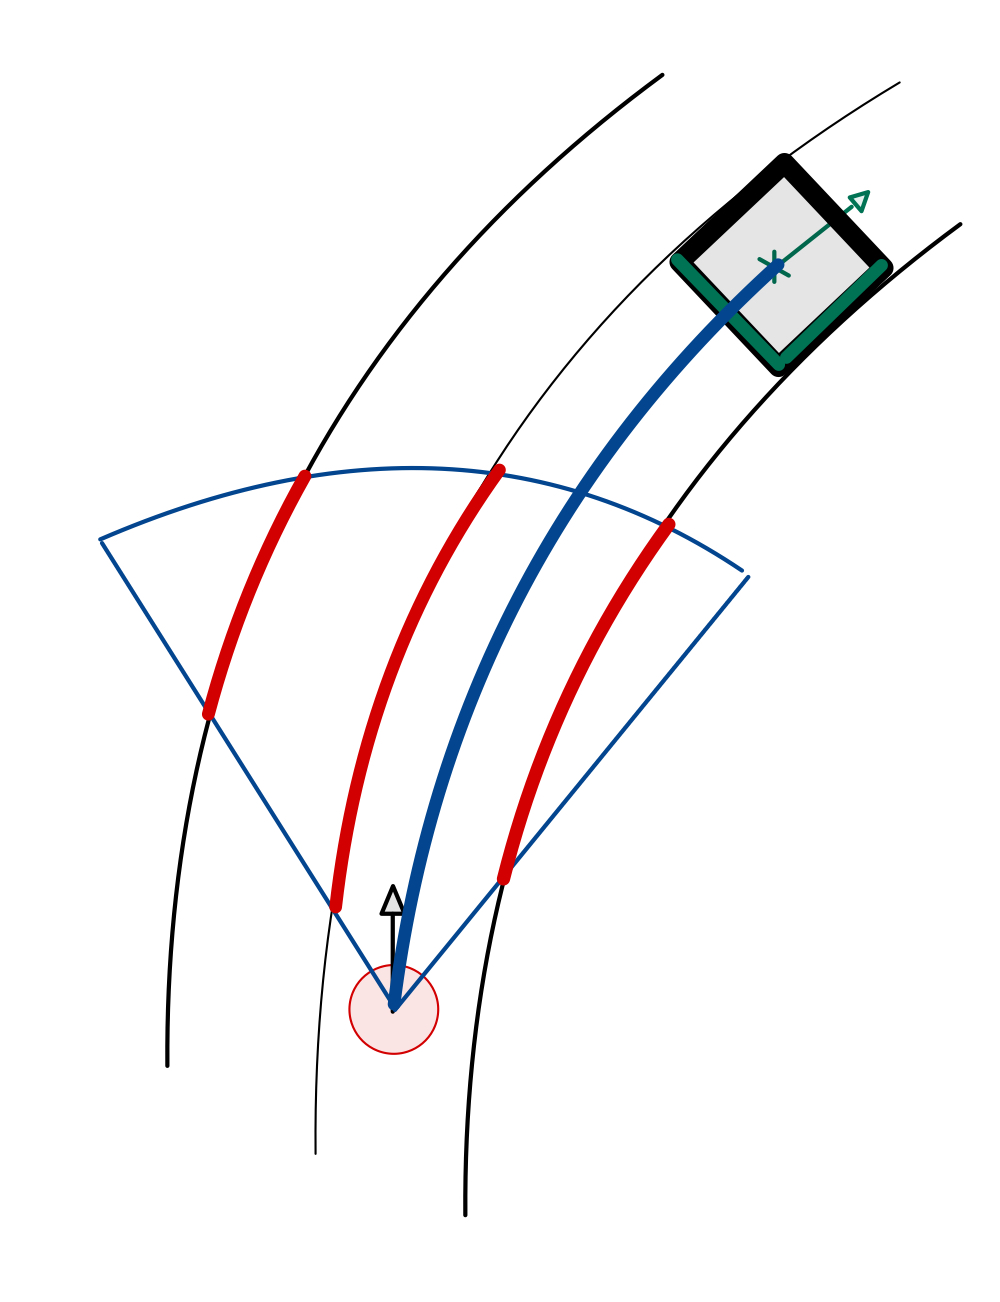
\includegraphics[width=0.33\textwidth]{Pictures/finding goal in obstacle}
	\caption{uncertainty of predicted goals }
	\label{goaluncertainty}
\end{figure}


\subsection{Goal from map}

If the robot is running a SLAM algorithm during the first round, the goal can be extracted directly from the SLAM map afterwards. This is more efficient and provides goals that will always be on the road. Furthermore the distance, at which goals will be found can be increased, this results in higher speeds of the robot and/or lower planner frequencies.\\

To find a goal in the SLAM map a circle rasterization algorithm will be used, based on Bresenham rasterization \cite{ComputerGraphics}.\\

This algorithm finds every cell on a circular path around the robot and its associated value in the map. The values outside of a given FOV (field of view) can be eliminated. The remaining values with a larger likelihood than a configurable threshold will be reduced to one point by taking the mean value of them.\\

The orientation of the goal is determined by using the previously explained approximation algorithms.

\subsection{Concept}

Based on the previously proposed ways to determine goals, the concept pictured in figure \ref{posefinder structure} can be deduced.\\

\begin{figure}[H]
	\centering
	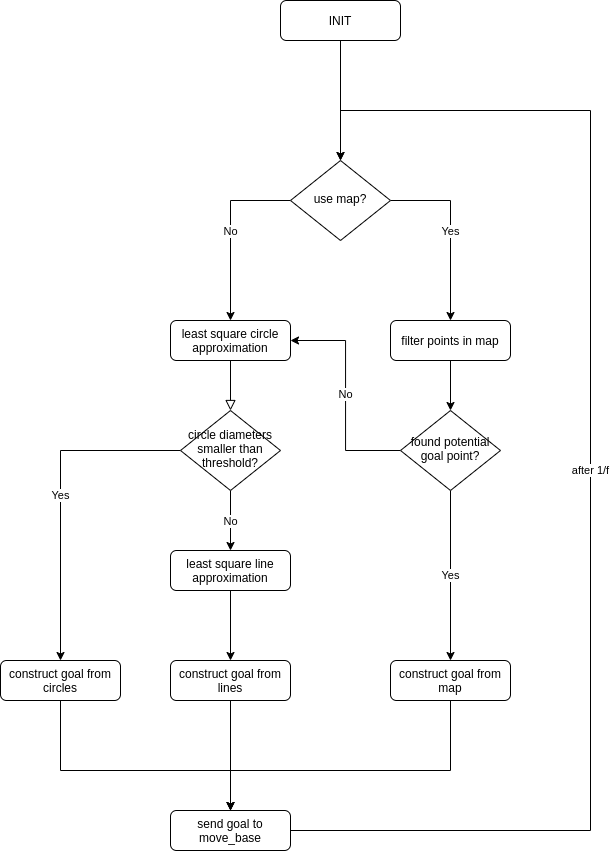
\includegraphics[width=.9\textwidth]{Pictures/posefinder diagram}
	\caption{PoseFinder internal structure}
	\label{posefinder structure}
\end{figure}

The goalfinding algorithms are ordered in a hierarchic structure based on their expected accuracy.

A accurate map of the surrounding offers the best potential to find feasible goals on the upcoming road, hence it has to be checked first, if a goal can or should be extracted from the map.

As described, every sections can be expressed by a circle segment. This approximation will have a higher priority than the line approximation.

Finally the line approximation will be checked and only, if the circle approximation generated circles with radii, that exceed a threshold for their trustworthiness.

The result of the chosen algorithm can be used to determine a goal that will be sent as an input to move\_base.

The goal found by the approximation, unfortunately is not certainly on the road. It could as well be in an obstacle or of the road, which would make complete navigation to the goal impossible. Hence this procedure will be repeated at a configurable frequency, so the robot will never reach one of the goals. 

The node is configurable using rqt\_reconfigure and the following parameters.

\begin{table}[H]
\centering
\resizebox{\columnwidth}{!}{%
\begin{tabular}{ l l l }
	
 \textbf{Parameter} & \textbf{Description} & \textbf{Range}\\
 CRadThresh & The Threshold for the radius of the circle approximation & 0.5-20 [m]\\ 
 GoalDist & The maximum distance at which a goal should be found & 0.5-20 [m]\\  
 GoalAngle & The maximum angle for the circle approximation higher priority than distance & 0.1-2 [$\pi$]\\  
 reductionradius & Max Distance at which points from the map will still be combined & 0.25-2.5 [m]\\  
 MapCostThresh & Threshold Cost Value for Map Data Extraction & 0-100\\  

\end{tabular}
}

\caption{PoseFinder parameters}
\label{posefinderparams}

\end{table}

\section{MarkFreeSpace}

Like described in the concept, the purpose of this node is to provide data to the SLAM algorithm as well as to the costmaps. This data consists from the points on the polynomials of the road detection in combination with the filtered points of the lidar scan.\\
Based on the possibility of the obstacle\_layer of the costmap to raytrace marked obstacles, it needs to receive a PointCloud2 that contains points from the polynomials of the road detection. If this pointcloud would contain the points of the lidar as well, the obstacle layer would remove the points of the road marking, if an obstacle is behind it.\\


For the SLAM algorithm both data sources need to be fused into one point cloud. Therefore, the points need to be transformed into the same frame and time, before being published.\\

The data of the dynamic cost layer has to contain more information. It is in the form of a point cloud and contains channel values for point individual inflation radius, min-cost and max-cost. By giving the layer point individual inflation parameters the node provides information about the cells on the left road marking that need to have inflated cost values and information about the points on the right road marking that should have a clear zone around them. Furthermore, the node provides points of obstacles that are on the road and clears the inflated cost around it. This cleared zone makes the generation of a path past the obstacle easier for the global planner.\\

The following parameters are offered for further configuration:

\begin{table}[H]
\centering
\resizebox{\columnwidth}{!}{%
\begin{tabular}{ l l l }
	
 \textbf{Parameter} & \textbf{Description} & \textbf{Range}\\
 MaxCost & Maximum cost of the left lane inflation & 0-254\\ 
 MinCost & Minimum cost of the left lane inflation & 0-254\\  
 LeftInflation & How far the inflation of the left lane overlaps the right lane & 0-1\\  
 RightRemoval & How much of the right lane will be cleared from cost & 0-1\\  
 ObstacleRemoval & Distance around obstacles on the road where no cost gets placed & 0-2 [m]\\  
 InflPointDistance & min Distance between inflated points 0 for only last & 0-5 [m]\\ 
 ClearPointDistance & min Distance between points that clear cost 0 for only last & 0-2 [m]\\   
\end{tabular}
}

\caption{MarkeFreeSpace parameters}
\label{markfreespaceparams}
\end{table}

\section{dynamic\_cost\_layer}
Enhancing to the plugins provided in the navigation stack this layer handles inflation of cells with a configurable cost decay and radius. While this seems to be similar to the provided inflation layer, this offers way more flexibility since it will inflate specific points by their individual radius and cost distribution and not just every lethal one by one fixed distribution.\\

This behavior can be used to inflate the left road marking in the global costmap to force the global plan on the right side of the road, which is the behavior defined in the concept. The plugin can also be used to inflate cells with zero cost, which is useful to guarantee a cost free right lane or to give some free space around obstacles located on the road.\\

The layer receives a point cloud on a configurable topic. This point cloud is expected to feature channel values for the inflation radius, the maximal and the minimal cost for each individual point.\\

Since it can not be assumed, that the incoming points will be in the frame of the costmap the points in the costmap have to be transformed into the right frame using tf2.\\

To minimize the computation load a Bresenham based algorithm for the circle rasterization will be used\cite{ComputerGraphics}. The point symmetry around the cell can be used to further minimize the computational load and only $\frac{1}{8}$th of the circle has to be computed. The rasterization process can be described by the following image.\\

\begin{figure}
	\centering
	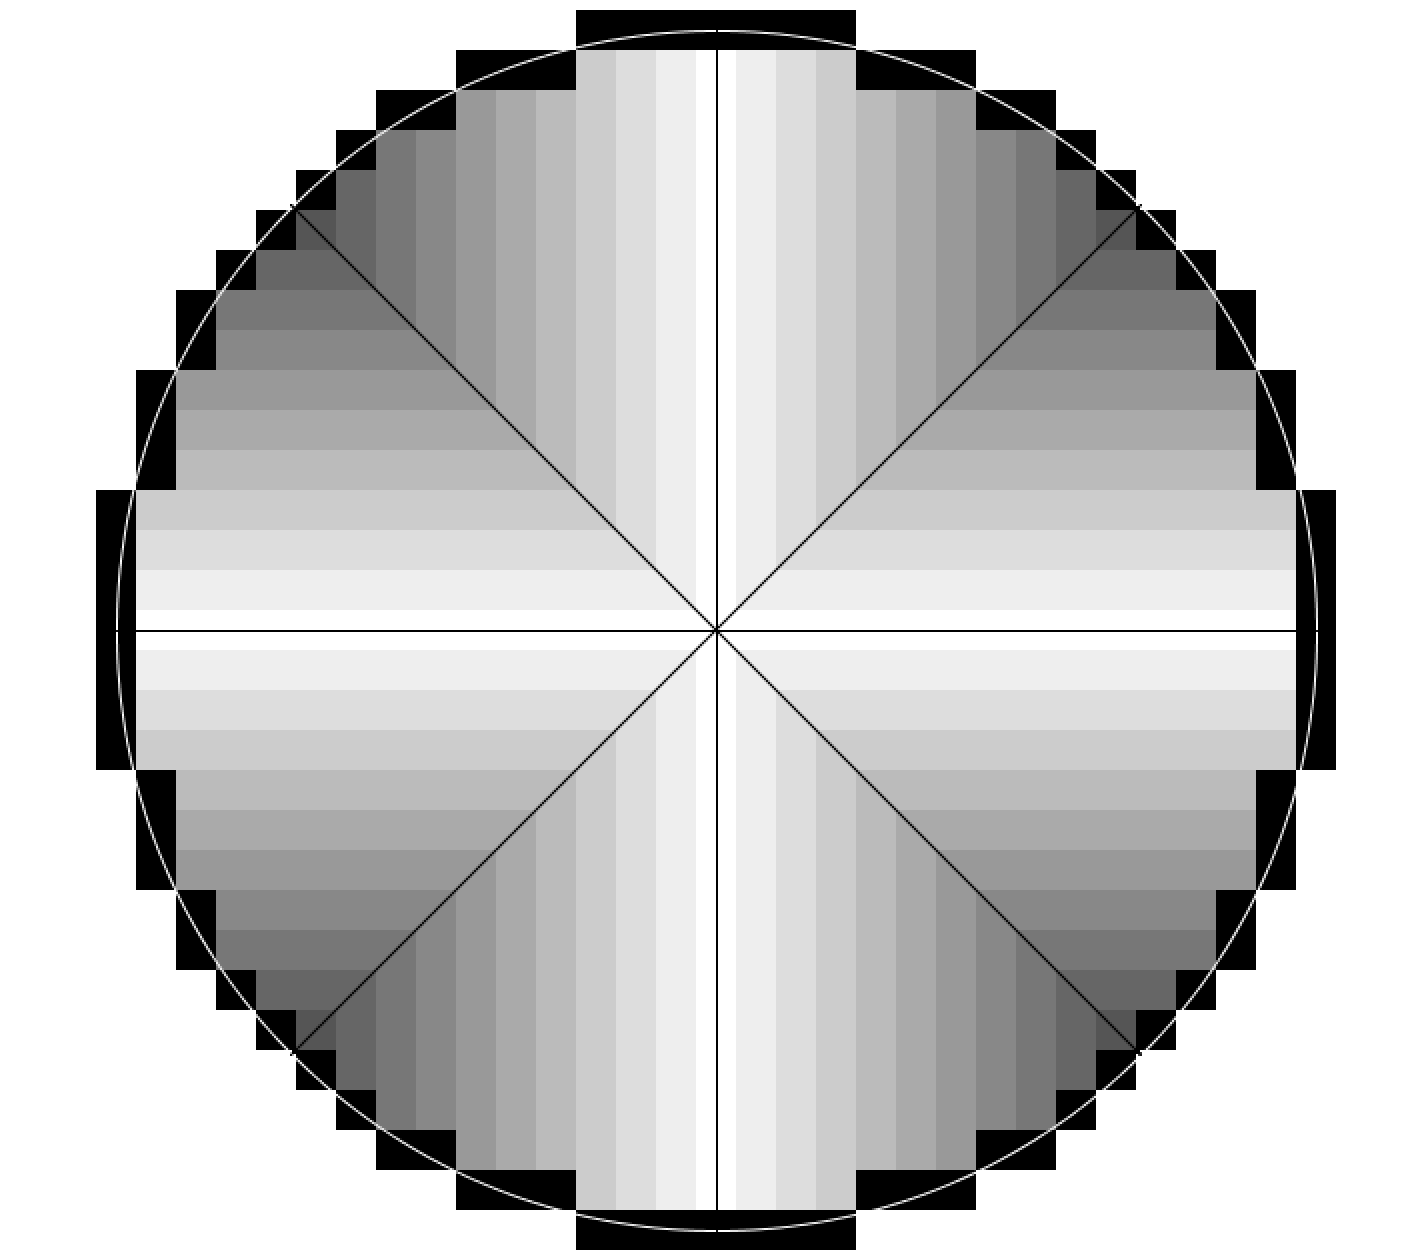
\includegraphics[width=.5\textwidth]{Pictures/rasterization}
	\caption{modified Bresenham rasterization with efficient surface filling}
	\label{rasterization}
\end{figure}


Adding to the typical behavior of the Bresenham rasterization the area of the circle will be filled using the point symmetry and by skipping overlapping points of the lines like in Figure \ref{rasterization}. Here it is visible, that every row with the same color is only calculated once and then projected in all eight octants. The black cells on the perimeter are the rasterized cells of the Bresenham algorithm.

The cells within the circles perimeter are filled with the cost specified for that point. For this the following linear decaying \nth{1} degree function will be used which requires the computation of the distance of the rasterized cell to the center of the circle.

\[cost(distance)=maxcost-distance*\frac{maxcost-mincost}{radius}\]\\
with: \[distance=\sqrt{cell.x^2+cell.y^2}\]

 Since this will still require the usage of a square root for each cell in the circle This will be optimized as well.\\

The goal here is to use a function that contains only the squared distance and not many other mathematical operators, which still represents a decaying trend. This requirement rules out every function with an odd degree, all functions with an x offset and the normal distribution. This leaves all functions with an even degree from which the \nth{2} degree function is chosen to reduce square operators. The comparison between the two functions can be seen in the picture below.

\[cost(distance)=maxcost-distance^2*\frac{maxcost-mincost}{radius^2}\]\\

\begin{figure}[H]
	\begin{center}
	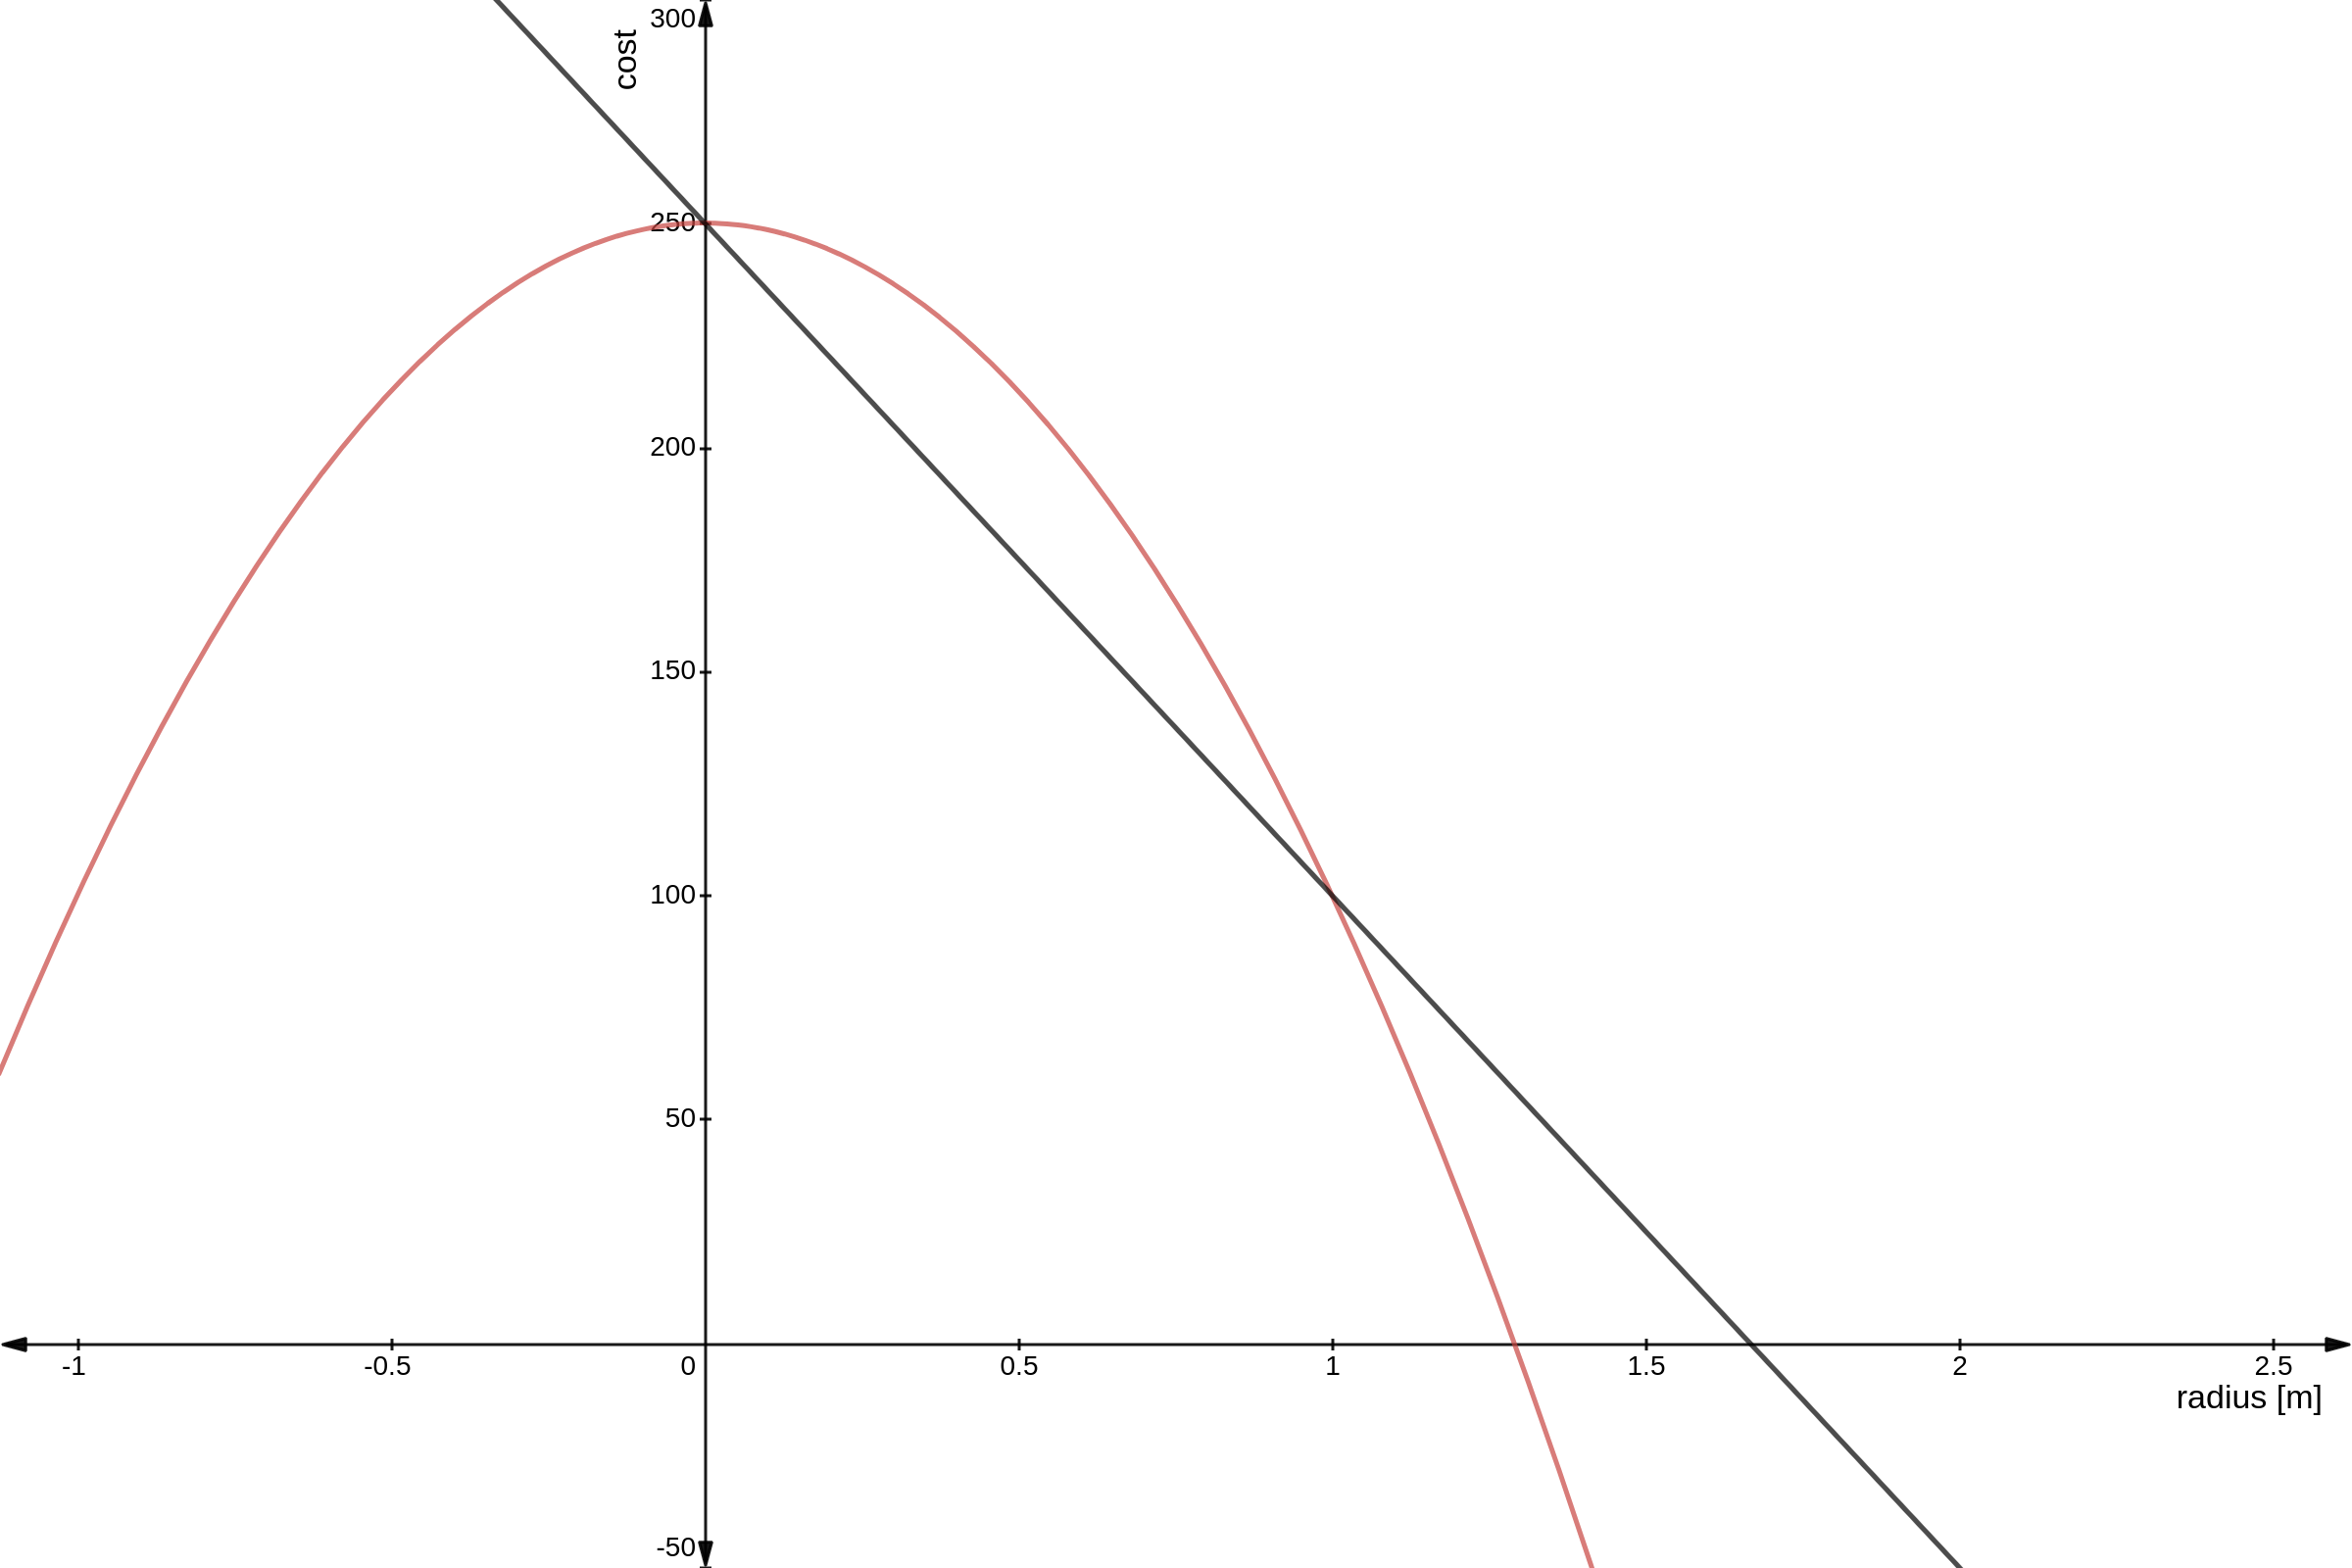
\includegraphics[width=140mm]{Pictures/linear cost comparison}
	\caption{cost distribution comparison with maxcost=250 mincost=100 radius=1}
	\end{center}
\end{figure}

When adding the inflation around points, the maximum of the calculated cost value and the current value of the cell in the costmap is set.
This leads to a problem, when trying to clear zones in the costmap, since then the minimum cost of the two needs to be set. Therefore setting zero as the cost value has the privileges for overwriting high cost values in the costmap.
 To prevent the cleared cells from being overwritten by the inflation of the next point, the clearing points have to be the last points in the input point cloud.


The layer can be configured individually for the costmap using rqt\_reconfigure and the following parameters.

\begin{table}[H]
\centering
\resizebox{\columnwidth}{!}{%
	\begin{tabular}{ l l l }
	
 	\textbf{Parameter} & \textbf{Description} & \textbf{Range}\\
 	enabled & Whether to apply this plugin or not & [bool]\\
 	point\_topic & The Topic of the PointCloud containing Points and channel values for inflation radius & [string]\\

	\end{tabular}
}
\label{dynlayerparams}
\caption{dynamic\_cost\_layer parameters}
\end{table}



\section{SLAM}
There are numerous lidar based SLAM packages available for ROS, but with the defined restriction of being able to use both, the points extracted from the road detection, as well as the lidar scan, most of the lidar based SLAM algorithms wont work since they only accept one lidar scan.\\
This rules out the popular options for lidar based SLAM like gmapping and HectorSLAM and the well documented package Google Cartographer will be used based on its flexibility in regards to robot configurations.\\
This package comes with an advantage of being based on loop closure, which might be useful when driving rounds in a circuit stile environment. The robot will drive the same route over and over again and thus the map could get more and more reliable over time even though the data is similar for different parts of the circuit and therefore not idal for the use with a SLAM algorithm.\\

Google Cartographer accepts numerous different input types including both point clouds and lidar scans. Additionally Google Cartographer can use provided odometry, as well as IMU data to improve the quality of the map.\\










%\chapter{Configuration and Testing}
\label{configurationandtesting}


This chapter will contain the configuration of all nodes of the concept. In addition the newly developed nodes have to be tested as well as the entire navigation concept.

The nodes of the system are highly interconnected, therefore it is hard to test nodes while eliminating the error of others.

\section{URDF and Robot State Publisher}

The URDF model is based on the model of Christen Lofland, who created this for his own open source project\cite{chrisl8}.\\

Unfortunately this model has been created to generate the fixed transforms of a real model only, so it does not have moveable joints for the wheels or any plugins for sensors and the differential steering. In addition to that it uses .stl files for both visual and collision volumes which results in unpredictable collision distances.\\

To keep the model as simple as possible one common xacro file is used, that loads the individual files for the following parts:
\begin{itemize}
	\item Arlo body
	\item camera
	\item lidar
	\item imu
	\item gazebo plugins for all sensors and differential drive
\end{itemize}

All of the files are xacro files in contrast to pure urdf so parameters and macros can be used, which makes the robot model more flexible.\\

The plugins for gazebo have not been included in the individual files so the urdf can be used for real robots with a similar sensor setup without big modification but just with the exclusion of the plugin file.

The resulting Robot then looks like pictured in Figure \ref{arlourdf}.

\begin{figure}
	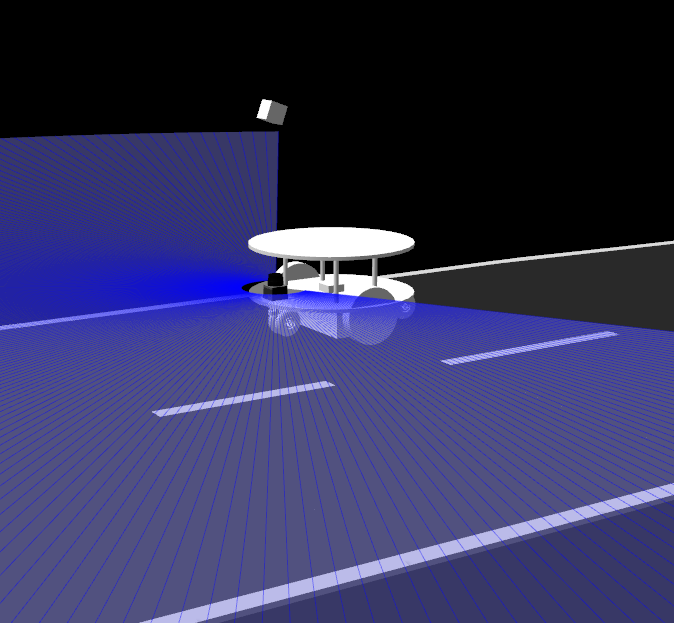
\includegraphics[width=\textwidth]{Pictures/arlourdf}
	\caption{ArloBot URDF with sensors and gazebo plugins}
	\label{arlourdf}
\end{figure}

\todo{add and ref tf tree of running system}

Using rqt\_tf\_tree the tf tree can be checked for conformity to ``REP 105'' and the concept.\\ 
The tf tree of the running concept is pictured in Figure \ref{}. As visible the fixed frame of the setup is ``map'' the following transform to the ``odom'' frame is published by cartographer. The transformation between the ``odom'' frame and ``base\_footprint'' then gets published by robot\_localization here named ``ekf\_se''.\\
The following transformations and frames are published by ``robot\_state\_publisher'' according to the URDF of the robot.

\section{Gazebo}
The setup of the simulation consist out of the modeling of the world, the conversion of the model into a sdf file and the general launch file.

As described in the concept the world will be modeled using the software blender.\\

\todo{rewrite blender problems}
The modeling itself is very straight forward since one segment of the road can be modeled and extruded along a closed path. Unfortunately the export of this model with the configured texture is not as intuitive and requires a work around.\\

Blender seems to not apply the texture if the model is exported directly as a colada file, so the file has to be exported as a Wavefront OBJ file. While gazebo can theoretically handle both formats the model editor of gazebo overrides the texture of the obj file permanentely.\\

When importing the OBJ file back into blender and exporting it again as a colada file the texture remains attached to the mesh. The model editor in gazebo overrides this texture as well, but in this case the applied texture can be removed in the generated sdf file and the road texture remains.\\

A important step is to set the road to static in the sdf file so it is not affected by the gravity of the simulation.

Using gazebo a .world file can be created, that includes a sun, the modeled road and a black ground plane so the robot does not drop into infinity, if it leaves the road.\\

The finished world then looks like pictured in Figure \ref{simworld}

The course of this road has been constructed so it features the following features:

\begin{itemize}
	\item left and right curves
	\item tight and wide curves
	\item long straight section
\end{itemize}

It will be the environment for most of the following tests.

\begin{figure}
	\centering
	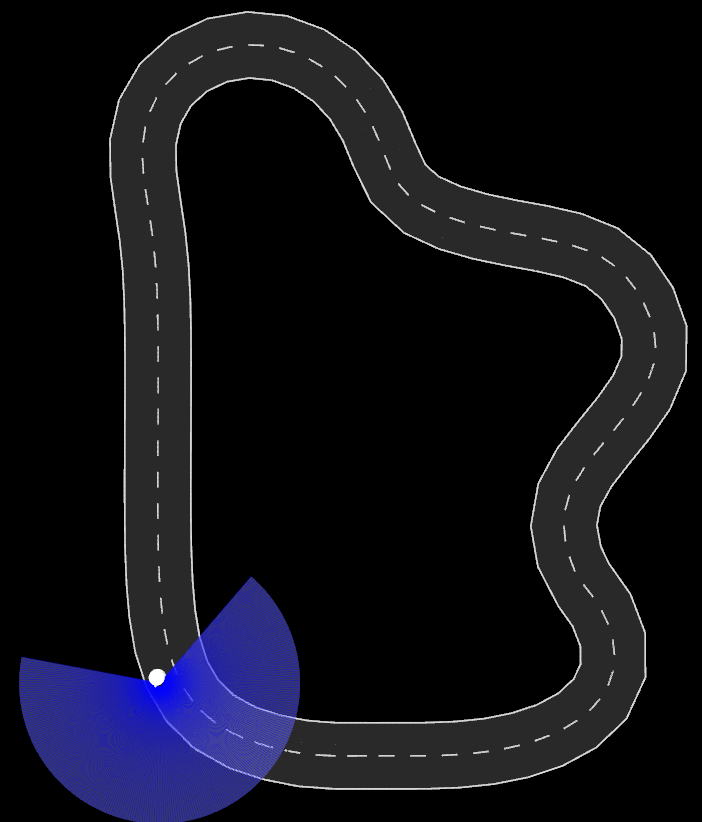
\includegraphics[width=.5\textwidth]{Pictures/test track}
	\caption{finished simulation world used for various tests}
	\label{simworld}
\end{figure}

Gazebo then can be started from a launch file by defining the generated world.\\

\subsection{Plugins}
The configuration of the sensor and drive plugins are fairly straight forward, based on the Tutorial page in the gazebo wiki\cite{gazebotutorial}.\\



While trying to simulate the original camera of the robot based on its datasheets (Appendix \ref{AppendixDataSheets}) and the calibration parameters, it is observable that not all parameters of the camera\_info message can be set in the sdf description of the plugin.

Overall it does not seem to be possible to mimic the original camera, hence the camera will be modeled without distortion with the assumption that a calibrated camera and image rectification packages like ``image\_proc'' would produce a comparable result.





\section{Filter}

As described the filter incorporate nodes that process the data so it can be used by the navigation concept. The following sections will cover the configuration of the individual nodes and their test setups.

Since the navigation highly relies on the data published by the nodes categorized as filters, these will be tested first.

\subsection{road\_detection}
The road\_detection provided by Prof. Dr. Stefan Hörmann consist out of the following six nodes of which some need configuration to work with the specific camera setup.

\begin{itemize}
	\item edgeDetector
	\item edgeProjector
	\item LineFinder
	\item LineTracker
	\item RoadDetector
	\item RoadRecordEvaluation
\end{itemize}

The edgeDetector is the first node of the package and extracts the edges from the picture using canny filters. Here the expected line width in pixels has to be configured. The easiest way to determine the width is to run the node and take a look at the picture published on the topic ``/roadDetection/image\_edges''. Then rqt\_reconfigure can be used to raise the maxLineWidth parameter, until the entire line of the road is visible in the filtered picture. In the case of the simulation the adjustment of the canny thresholds is not required, since the environment has only black and white colors and no greyscale.\\

The edgeProjector has the task to project the image on the 2D surface and therefore must know the position and orientation of the camera relative to the ground. While doing so it rectifies the image according to the provided camera information, which should contain the calibration parameters of the setup.

To get a reliable result from the ``LineFinder'' the amount of tiles in x and y has been increased to get more precise lines from the internally used hough transformation.\\
In this scenario the robot drives on a wider road than usual for the carolo cup, so the parameter maxSegmentDistance has been increased to 0.9 m so the line segments of the middle line will still be matched to the same line.\\
When the robot drives around a tight corner the road often starts at an angle relative to the robots x axis. The parameter ``maxStartAngleDiff'' has been increased to 75° to get more coverage in this case.\\

While configuring the road detection the first step is to configure the orientation and position of the camera in the node``edgeProjector'' according to the definition in the urdf file. In addition to that the camera picture has to be cropped so the robot is not visible anymore in the picture.\\

In the ``LineTracker'' Node the distance, at which lines should be evaluated needs to be set, so the node does not see the edge of the picture, in which the distortion has the largest effect.\\


The RoadDetector Node needs an estimate for the lane width as a min and max value and a maximum angle between two individual road markings. These values are obviously specific for the environment.\\

\subsection{MarkFreeSpace}

As discribed in the selection, this node has the task of supplying individual point clouds to the following three nodes:

\begin{itemize}
	\item dynamic\_cost\_layer costmap plugin
	\item obstacle\_layer costmap plugin
	\item cartographer
\end{itemize}

The cloudes for the obstacle\_layer and for cartographer are just different combinations of the points from the road detection and the lidar scanner this does not have any configuration options and is very basic and therefore will not be covered in detail.

The dynamic\_cast\_layer of the global costmap will only inflate every point by the specified parameters of a cost distribution, so this node has to build a message as described in the selection section of this node.\\

Since the data that needs to be sent to the costmap layer originates from two different sensors they have to be synced in time, meaning the newer signal needs to be transformed back in time to the last occurrence of the older signal and transformed in the base frame of the robot.\\

After that the points can be merged into the point cloud. While doing so the cost parameters of the individual points gets set aswell. If a specific section needs to be removed out of the costmap layer these points will be appended to the end of the point vector of the pointcloud so they will not be overridden by other inflated points.\\

To keep this node flexible in regards to the environment, the inflation radii for all points are derived from the current road width, which is supplied by the road\_detection and can be configured using rqt\_reconfigure. 
In addition to that the distance between the inflated points of each road marking and the min and max values of the cost distribution can be configured.


\section{Cartographer}
The goal of this node is to produce a map that gets more reliable over time.\\

Unfortunately the data available for Cartographer is very self simillar, meaning a straight road will allways look the same and therefore does not have sufficient features for proper loop closure. In contrast to the points from the road detection the lidar can actually supply such features and will therefore be a good improvement for the resulting map.\\

But it is not guaranteed that the lidar will even sees anything the SLAM algorithm has to work with the points of the road detection only aswell.

The basic configuration of cartographer is purely based on the setup of the robot. In this case cartographer is supposed to use lidar and the points of the road detection at the same time. To reduce the amount of times one of the sensor doesn't see anything these will need to be merged in the markfreespace node and cartographer will receive one PointCloud2 only.\\
To improve the map further the odometry supplied by the robot\_localization package is used as an input, aswell as the IMU.

Furthermore cartographer will be set to 2d map building.


\subsection{Tuning}
With the basic configuration cartographer is not able to provide a reliable map and a tuning procedure has to be performed. Here the general recommendation of the tuning guide should be followed, which states to tune local SLAM first and disabling global slam while doing so \cite{cartographertuning}.
To tune the local SLAM the parameter of the tracjectory builder have to be adjusted.\\
The trajectory builder contains a scan-matcher, which will compare incoming sensor data and tries to align it with each other as good as possible. This behavior can be tuned by configuring the size of the linear and angular search windows and the weight for the rotation and translation of the incoming scans.\\
One more important setting is the size of the sub maps. These can be adjusted by the amount of scans they contain. Since the submaps will consist out of the scan matched obstacles it is important to set the size of the submaps not to high, if the incoming data will be very self simillar. Otherwise the scanmatcher will combine too many scans while shifting them over each other since they look so simillar. This results in both rotational and translational error.\\
As soon as the local SLAM produces a reliable result after multiple rounds of the robot the global SLAM can be activated and tuned.\\

The global SLAM has two options of combining the submaps the loop-closure, which will check, if the robot was at this spot already, and a scanmatcher, which will try to match the submaps to the current scan. For both of these the weights can be adjusted individually and like in the local SLAM the size of the window for translation and rotation can be adjusted. Reducing the window size to a minimum is aswell important when dealing with self simillar data, so the submaps will not be shifted on top of each other. The size should be chosen so the global SLAM can still correct errors of the individual submaps 
With these values and the submaps the global planner calculates constraints between the maps which will be valued between 0 and 1. These constraints can be blocked with a threshold value that will block constraints with a smaller value. like this the computation time can be drastically reduced and only the important constraints will be processed. Furthermore the weighting of the Pose of the odometry and the local SLAM can be adjusted, which can be usefull with bad odometry.

\subsection{Testing}
Testing of the SLAM will mostly consist out of a Black-Box Test meaning the only things that will be observed is the output and therefore the map.
The SLAM will be tested in the following cases:
\begin{itemize}
	\item Data purely from the road detection.
	\item Data from road detection and lidar scan with obstacles on the side of the road.
	\item Long duration test with both road detection and lidar scan with obstacles on the side of the road.
	\item Data from road detection and lidar scan with obstacles on the road.
\end{itemize}

During all of these test the navigation will solely work with the predicted goals since it is yet unsure if the SLAM map is even usable. Furthermore the same tuning will be used for all tests.\\



\section{PoseFinder}



\section{Costmaps}
Based on the fact that both planners are responsible for different tasks the configuration of the individual costmaps need to fulfill different tasks too. The requirements of the two planners will be compared in order to determine the configuration of their individual costmap.\\

As described in the theoretical knowledge of this thesis the costmap are structured in layers. This means that the data can be evaluated by different plugins before it will be combined into the real costmap.\\

It makes sense to first take a look at the general behaviour, that both planners share. In this case it is obstacle avoidance. This means that the lethal obstacles need to be marked in both costmaps.\\

To implement this the provided plugin obstacle\_layer can be used. It will take incoming sensor data (sensor\_msgs::PointCloud or sensor\_msgs::LaserScan) and mark the points in the costmap.\\

Since the data here comes form the road detection and a lidar and both have a certain resolution it is unsure, if the result of a scanned obstacle in the costmap is actually a closed line or just points, since this highly relies on the resolution of the sensors and the costmap.\\

To fill theses gaps in the costmap the provided plugin inflation\_layer can be used. It will inflate only the lethal obstacles in the costmap with a configurable cost distribution.\\

This setup is already enough for the local costmap, where as the global planner needs to fulfill the quest of changing lanes if necessary but all-ways preferring the right lane. For this a custom plugin will be needed that makes the transition to the left lane more expensive but still possible.


The final layer plugin setup of the costmaps results in the following:

\textbf{global costmap}
\begin{itemize}
	\item obstacle layer
	\item inflation layer
	\item dynamic cost layer
\end{itemize}

\textbf{local costmap}
\begin{itemize}
	\item obstacle layer
	\item inflation layer
\end{itemize}

The costmaps will both have the same size that should allways be larger than the distance, at which the goalfinder searches for goals.

Since both costmaps are rolling window costmaps they will reference the continuos frame ``odom'' and move with the frame ``base\_footprint''.

Counterintuitively the robot radius needs to be set smaller than the robot actually is. Otherwise the slightly moving obstacles collide with the footprint and the global planner can not produce a valid path that the local planner can follow.\\
This footprint is only considered by the global planner, which is only required to provide a rough path. The local planner has its own setting for a footprint, therefore the obstacle avoidance will still work as expected.

The last remaining settings are the resolutions and the frequencies of the costmaps, which are chosen based on the performance of the navigation and the computational load.


\section{Planners}

\subsection{global\_planner}
\label{globalplannertest}
There is not much room for configuration, when it comes to the global\_planner of the navigation\_stack. Probably the most important step for computation load is the choice of a planning algorithm.\\
The two algorithms that are offered by the global\_planner node are Dijkstra and A*.\\

\begin{figure}[H]
	\begin{subfigure}{.5\linewidth}
		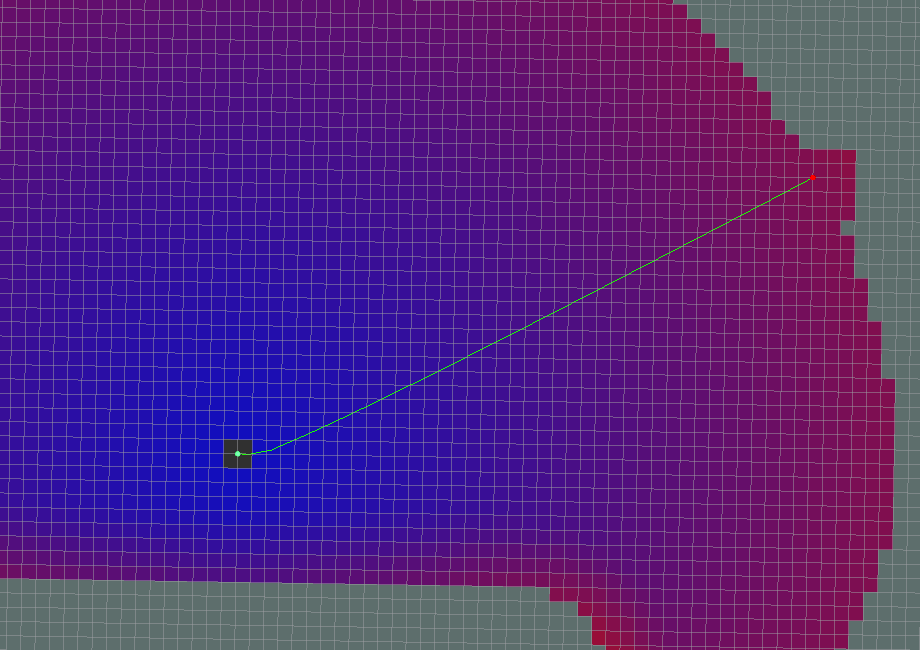
\includegraphics[width=\textwidth]{Pictures/Dijkstra}
		\caption{Dijkstra}
	\end{subfigure}	
	%\hskip2em
	\begin{subfigure}{.5\linewidth}
		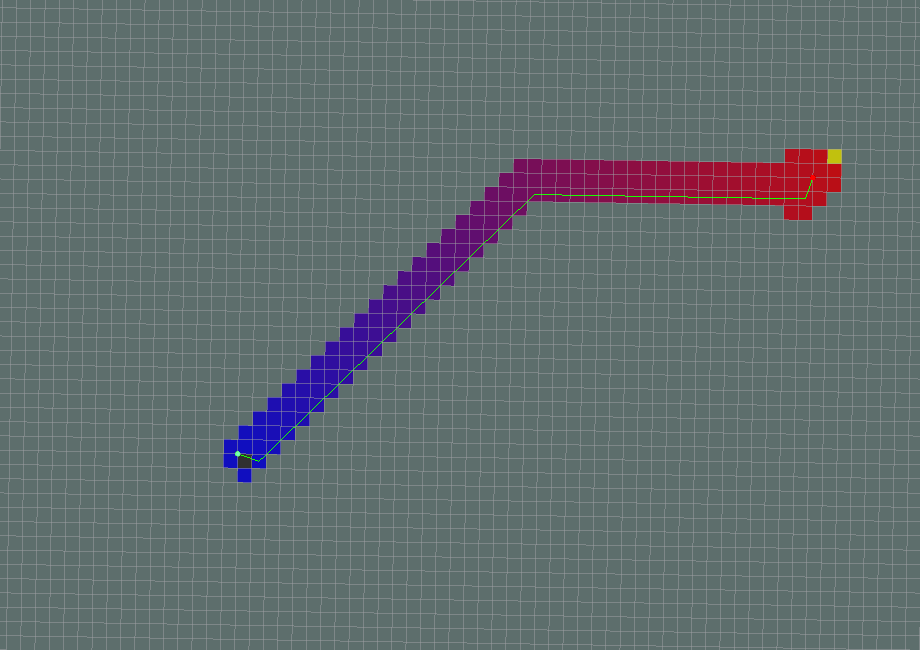
\includegraphics[width=\textwidth]{Pictures/AStar2}
		\caption{A*}
	\end{subfigure}

	\caption{planning algorithm comparison (grey cells are not observed)\cite{globalplanner}}
	\label{plannercomparison}

\end{figure}


It is obvious, that A* is much more efficient in this use case since the robot will mostly go straight or in a slight curve. Therefore A* will be chosen for the global planner.\\

Another important setting is necessary since the global costmap is used as a rolling window costmap. The global\_planner will be default outline the global costmap with lethal cost to prevent the global planner to plan outside of a fixed costmap. This behaviour results in artifacts, after the map has moved together with the robot which hinder the planners from finding a path.

\begin{figure}[H]
	\centering
	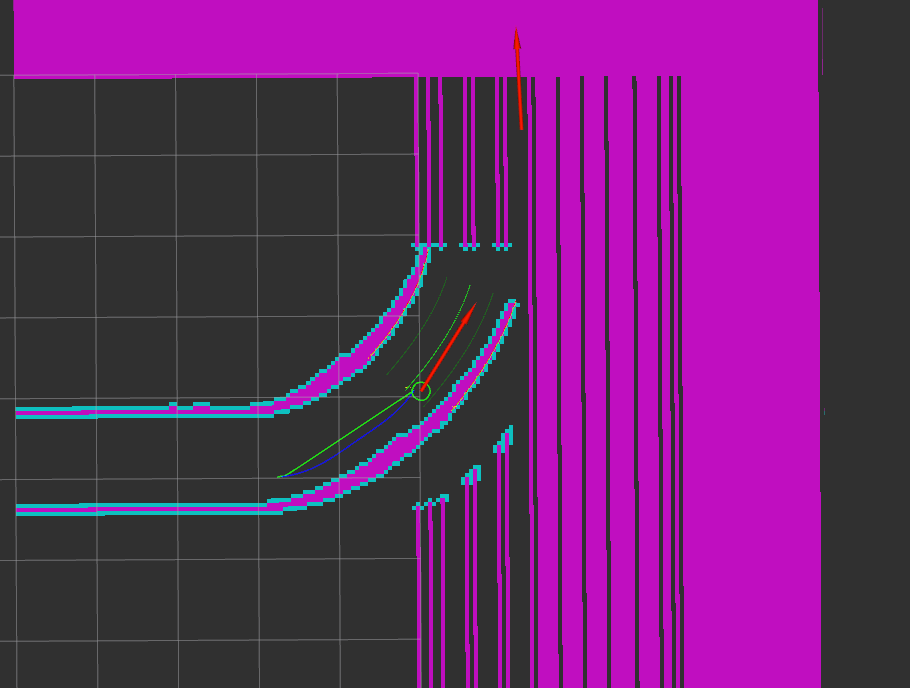
\includegraphics[width=\textwidth]{Pictures/borders}
	\label{boardererror}
	\caption{global planner border error}
\end{figure}

To prevent this behavior the not documented parameter ``outline\_map'' has to be set to false. The default value of this parameter is therefore changed in the forked version of the navigation stack.

To make planning easier the parameter ``cost\_factor'' can be reduced. This parameter multiplies the cost of every cell in the costmap before planning which
 would make the gradually decreasing cost of the dynamic\_cost\_layer redundant.
 
 
 While using the global\_planner plugin a bug during the potential field calculation has been observed as pictured in \ref{potentialfield}. This bug causes an error of the planner, since it is not able to resolve a path, even though the potential field exists. Which therefore leads to the robot continuing to drive with the same velocities,  until the planner manages to construct a valid potential field again. In this moment the robot often leaves the right lane even though there is no obstacle infront of it.
 
 This bug has been reported to the developer of the plugin.
 
 \begin{figure}[H]
 	\centering
 	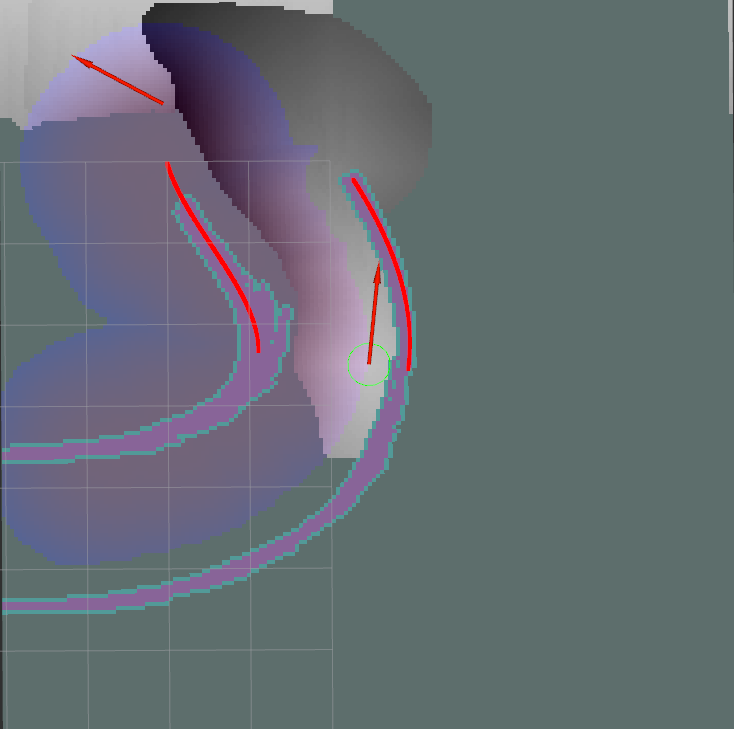
\includegraphics[width=.7\textwidth]{Pictures/out of bounds}	
 	\label{potentialfield}
 	\caption{Potential field generated by global\_planner plugin}
 \end{figure}


\subsection{teb\_local\_planner}

Like the global planner the local planner has to be configured to comply to the tasks the local planner has.

A good starting point for the configuration are the example configurations in the repository of the developer of the planner\cite{tebtutorials}. They offer base configurations for both differntial drive and car like, aswell as omnidirectional robots.\\

Unfortunately teb\_local\_planner only considers lethal cost and without any configuration would follow the global path very loosely resulting in e.g. cutting corners.\\ 

To give the planner a tendency to follow the global planner closer the option ``viapoint'' can be used. This allows to set points at a configurable distance to each other on the global path, that attract the local path and therefore pull the local path and the robot to the correct lane. The attraction of the local path through the via points is then tuned so the robot drives roughly in the middle of the right lane, when no obstacle is on the road, but still can separate itself from the global path, when avoiding obstacles.\\

The parameter ``max\_global\_plan\_lookahead\_dist'' controls how much of the global plan is actually considered by the local planner. This parameter highly influences the computational load when setting the distance to larger values. Using shorted distances results in oscillations while driving straight, which is caused by the jumping global path.

During testing teb\_local\_planner produced mostly good and feasible paths, but sometimes it generated loops along the global path, that would result in the robot turning in spot, before it follows the global path further. This leads to the robot changing the driving direction since after half of a turn the PoseFinder finds new goals, that are feasible.\\

To suppress this behavior the weighting of the time component has been increased so the internal forces that contract the elastic band increase. This reduced the occurrence of this scenario significantly, but the local path takes longer, until it is on the right lane again, since the distance to the global path is now weighted less relative to the weight of the time component.

\section{Odometry test}
The odometry is a key component in the navigation concept, since it will be used by multiple nodes and is the representation of the robot's position in its environment.\\

Especially differential robots tend to have rotational error, when using the wheel-encoders to generate the odometry, since the wheels are forced to slip when the robot is turning.\\

To test the quality of the odometry the robot will be placed in the world pictured in Figure \ref{simworld}. Now the robot is supposed to drive one round, during which the odometry of the robot will be tracked.\\

In theory the trace of the odometry should be closed perfectly, after the robot performed its first round.\\

\section{Lidar test}
The lidar is the only sensor, which detects static obstacles in the surrounding of the robot. Hence the quality of the data has to be checked.

To test the performance of the simulated lidar the robot will simply navigate in the world pictured in Figure \ref{simworld} and detect obstacles along the road.\\

The quality of the data will be observed by looking at the raw data, aswell as the costmap, that receives the measurements of the lidar.\\

The evaluation of the costmap is necesarry, since it will mark measurements of the lidar as lethal. With increasing noise the marked obstacles will be less precise, therefore the lidar has direct influence on the performance of the navigation even when obstacles are not on the road.

The main focus of this test is sensor noise, since the gazebo sensor plugin is configured based on the data sheet of the real lidar.
\todo{appendix lidar and camera data sheets}

\section{road\_detection test}
As the road\_detection is the only data source providing informations about the road it is crucial for successful navigation.

To check if the roadDetection offers good enough results a long duration test will be performed, during which the output of the roadRecordEvaluation node will be monitored, which outputs the relation between the amount of recognized road and overall attempts to find a road.\\

The robot will navigate on the course pictured in Figure \ref{simworld} until the output of the roadRecordEvaluation settles to a reliable result.

\section{SLAM test}
The SLAM algorithm chosen for the the concept is used in a very uncommon way, since it is not only receiving input from a real range finding sensor, but as well from the road detection.

The data from the road detection is very self similar, meaning that for example a straight section of road will always look very similar independent of its position. The lack of details in the data from the road detection might complicate cartographers scan matching.

\textbf{Data purely from road detection:}\\
The reason for this test is to check if the SLAM algorithm can handle Mapping with as least information as possible. This will make loop-closure difficult and cartographer has to work with the self simillar data only.\\
The aim is, that the robot can drive multiple rounds, on the track and cartographer produces an optimized map with little unmatched submaps and well connected road markings.\\

\textbf{Long duration test with both road detection and lidar scan with obstacles on the side of the road:}\\
Cartographer seems to not merge old submaps but process all of them allways, which will progressively increase computational load. Since the SLAM is supposed to be used during mapping this can become important with a lot of sensor inputs that offer constraint potential and long runtime.
The same setup as in the \nth{2} test will be used but the focus is on the moment, at which cartographer cannot optimize in real time caused by too many submaps and constraints.\\


\textbf{Data purely from localization and lidar scan with obstacles on the road:}\\
This test is meant to be the worst case for the SLAM algorithm during navigation. The purpose is to check how cartographer handles data loss during obstacle avoidance and lane swapping.
The obstacles will be placed in two corners and therefore in the edge case where the camera has the worst chance of seeing the road because of the steering angle, aswell as on the straight section of the road to cover the case where the camera can not see the road during merging on an other lane. Furthermore the obstacles will be placed far enough apart so the lidar has only vision on one at the same time.\\


\section{complete system test}

After the previous tests the entire concept has to be tested in order to check, if the concept works as anticipated.

Autonomous navigation in the following test scenarios will be performed:

\begin{itemize}
	\item no obstacles
	\item obstacles on left lane
	\item obstacles on right lane
\end{itemize}

During all test the following criteria will be monitored aswell as any unexpected problems during the test:

\begin{itemize}
	\item distance to the right lane when no obstacle is close
	\item obstacle avoidance distance to object
\end{itemize}

For these tests the exact position of the obstacles and the robot will be used for evaluation. This allows to determine the exact distance between the robot and obstacles, aswell as if the robot is still on the road. The distance to the right lane will be determined by using the polynomial provided by the road detection. A so called ``avoidance'' starts when the robot is just slightly over the middle line, without any hysteresis.

As defined in the rules of the carolo cup the merging onto the right lane during the obstacle avoidance is supposed to take place within the next two meters after an obstacle \cite{carolocup}.

In all tests the robot will drive multiple rounds if possible to produce reliable results. The tests will be performed in the environment pictured in Figure \ref{simworld}.\\














\chapter{Results and Discussion}
\label{resultanddiscussion}


This chapter covers the results and the discussion of all tests formulated in Chapter \ref{configurationandtesting}. In addition potentially needed optimization steps will be highlighted.
\section{Odometry test}

When looking at the odometry published by the differential drive plugin during the test in Figure \ref{wheel odom} it is noticeable, that the measurement has a huge rotational error, which is expected since the wheels always slip slightly when turning a differential drive robot.
\todo{picture including true odometry}
\begin{figure}[H]
	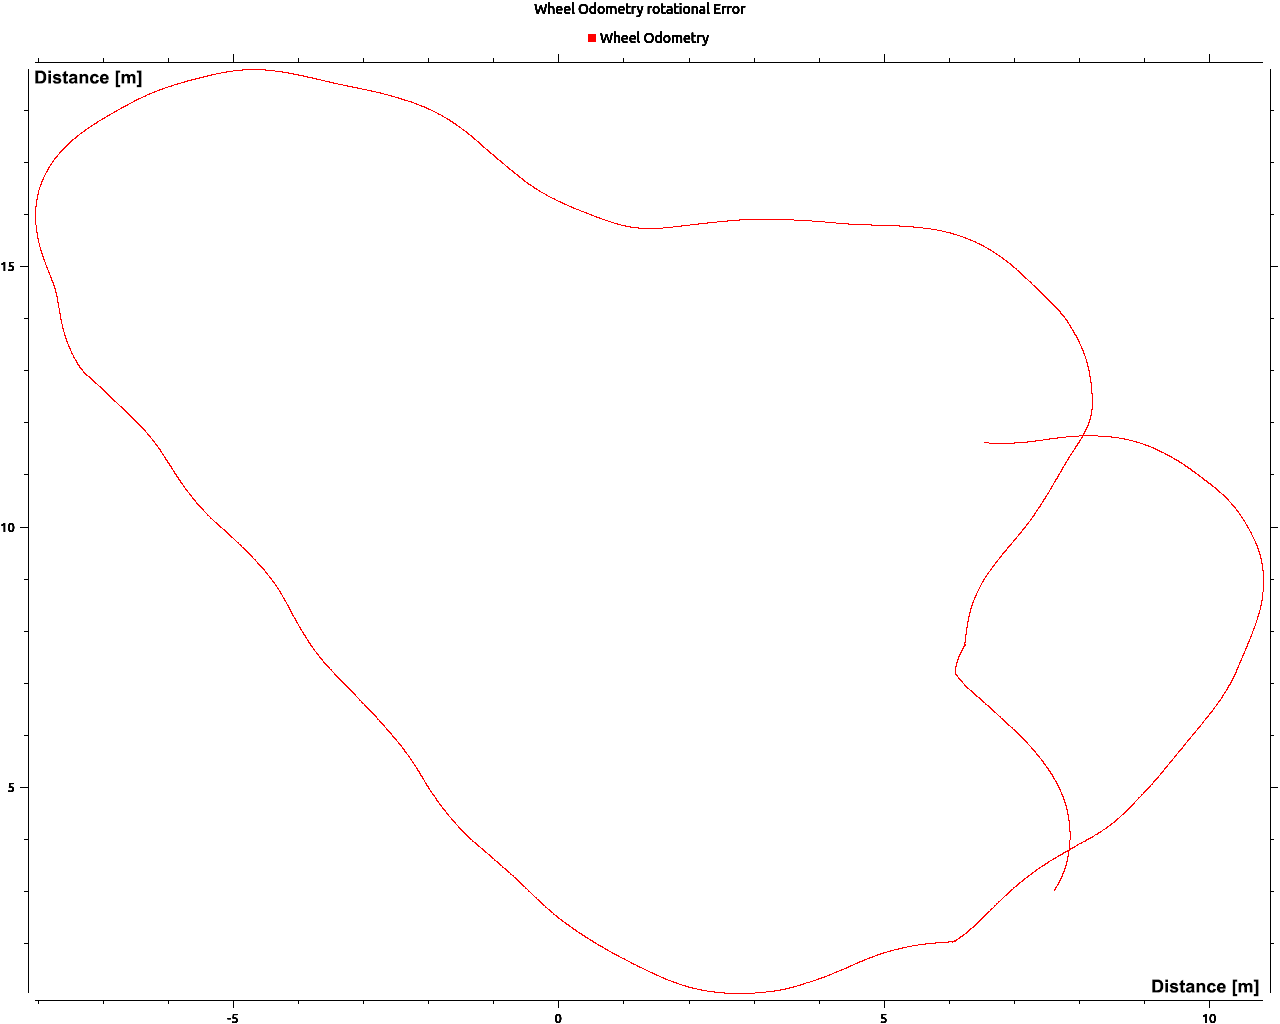
\includegraphics[width=\textwidth]{Pictures/rot error}
	\caption{Odometry Test result}
	\label{wheel odom}

\end{figure}

The quality of the odometry obviously is not sufficient and has to be improved.

\subsection{Optimization}
Since the odometry is found to not being sufficient for the navigation the following optimization approach will be tried and further testing will be performed. The test scenario will be remain the same.

To improve the odometry the ROS package robot\_localization can be used. It provides an extended kalman filter for the fusion of sensor data for odometry.\\

To reduce the rotational error, an IMU (Inertia measurement unit) will be added to the robot configuration. Both, the imu and the wheel encoder will be fused by robot\_localization.

The IMU provides the following data:
\begin{itemize}
	\item orientation
	\item angular velocity
	\item linear acceleration
\end{itemize}

In this usecase the IMU is only supposed to measure data relevant for 2D operation roll, pitch and tranlation in z (axis according to to REP 103) will not be passed to the filter. 

The IMU is used for localization purposes, therefore the linear acceleration data is not interesting, since the accelerations would need to be integrated twice to be used for the pose. This would amplify every little error in the measured acceleration and will decrease the reliability of the odometry with increasing time.\\

Accordingly the only things fused from the imu are the yaw orientation and velocity.\\

Just like the IMU data the integration of the wheel-odometry data has to be discussed which consist only from linear and angular velocities, aswell as a pose derived from the velocities.\\

Here the most interesting part is the y velocity since the robot is relying on differential drive steering and therefore not able to have instantaneous y acceleration other than drift.\\

In contrast to the acceleration values of the IMU the y velocity will be included since according to Tom Moore (the developer of robot\_localization) it will give certainty that the robot has not moved in the y direction\cite{robotlocalizationconfiguration}. Obviously the x and yaw velocity has to be included aswell.

The position component of the wheel-odometry on the other hand will not be used, based on the fact that the position is already derived from the velocitys this would include the same data twice.\\

Unfortunately this does not solve the problem of the odometry correction yet. As visible in Figure \ref{pose comparison wheel odom + IMU} the odometry of the extended kalman filter has large jumps in it compared to the wheel-odometry. When observing it in real time the ekf odometry starts to drift and jumps back after a certain amount of time.\\
Looking at the linear velocities of both the ekf and the wheel odometry in Figure \ref{velocity comparison wheel odom + IMU} it is noticeable that the ekf filter does estimate a continuous acceleration, whereas the velocity of the wheel encoders actually decreases.\\



\begin{figure}[H]
	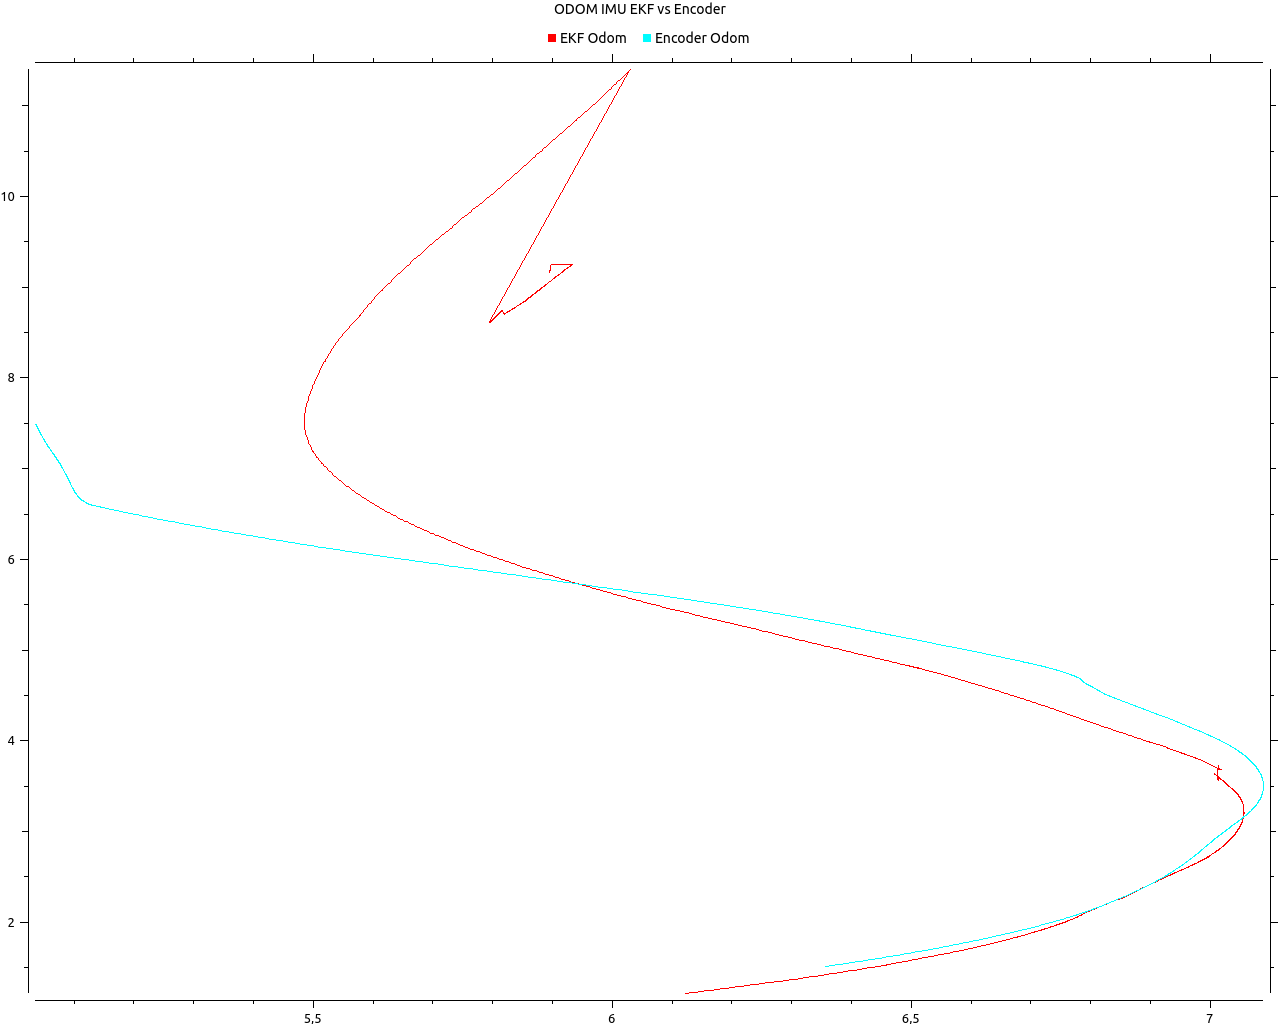
\includegraphics[width=\textwidth]{Pictures/odom pose comp}
	\caption{pose comparison wheel odom + IMU}
	\label{pose comparison wheel odom + IMU}

\end{figure}

\begin{figure}[H]
	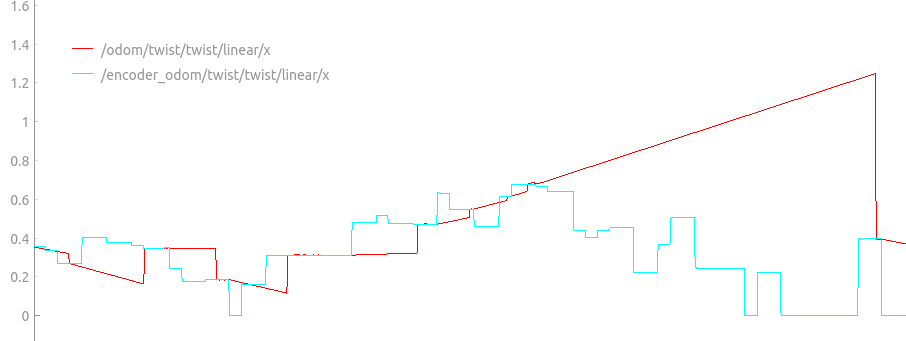
\includegraphics[width=\textwidth]{Pictures/comparison odom}
	\caption{velocity comparison wheel odom + IMU}
	\label{velocity comparison wheel odom + IMU}

\end{figure}


To fix this a logical approach is to include more data about the robots movement. Fortunately robot\_localization has an input for command velocities such as velocities produced by move base. While the command velocity does not provide any measurement in the real world the ekf filter can profit from knowing what the velocity actually should be.\\
It is very important to set the control timeout to a value that is larger than the cycle time of move\_base. Otherwise this will lead to translational offsets caused by too low estimate for the velocities like shown in Figure \ref{velwithcmd}.

\begin{figure}[H]
	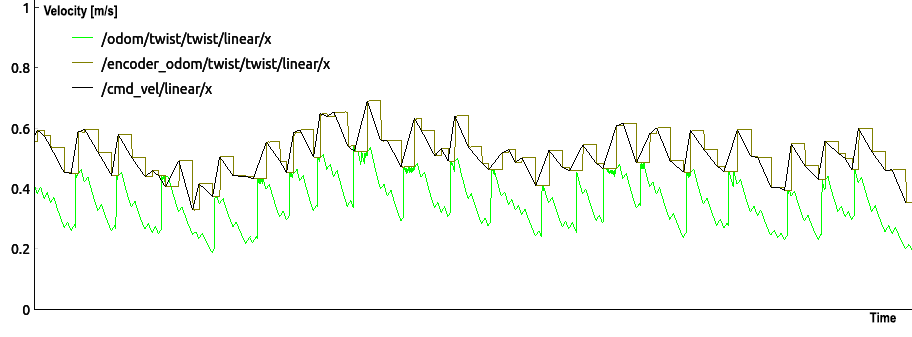
\includegraphics[width=\textwidth]{Pictures/velocity comp}
	\caption{velocity offset caused by too low control timout}
	\label{velocity offset}

\end{figure}


After the inclusion of the command velocity the acceleration limits in the configuration file of robot\_localization can be set equal to the limits in the local planner.

When observing both the pose and velocities again it is noticeable, that the odometry has drastically improved as pictured in Figure \ref{Odometry comparison wheel odomIMUcmdvel}, equally the velocities stay closer together as pictured in \ref{velwithcmd}.

\begin{figure}[H]
	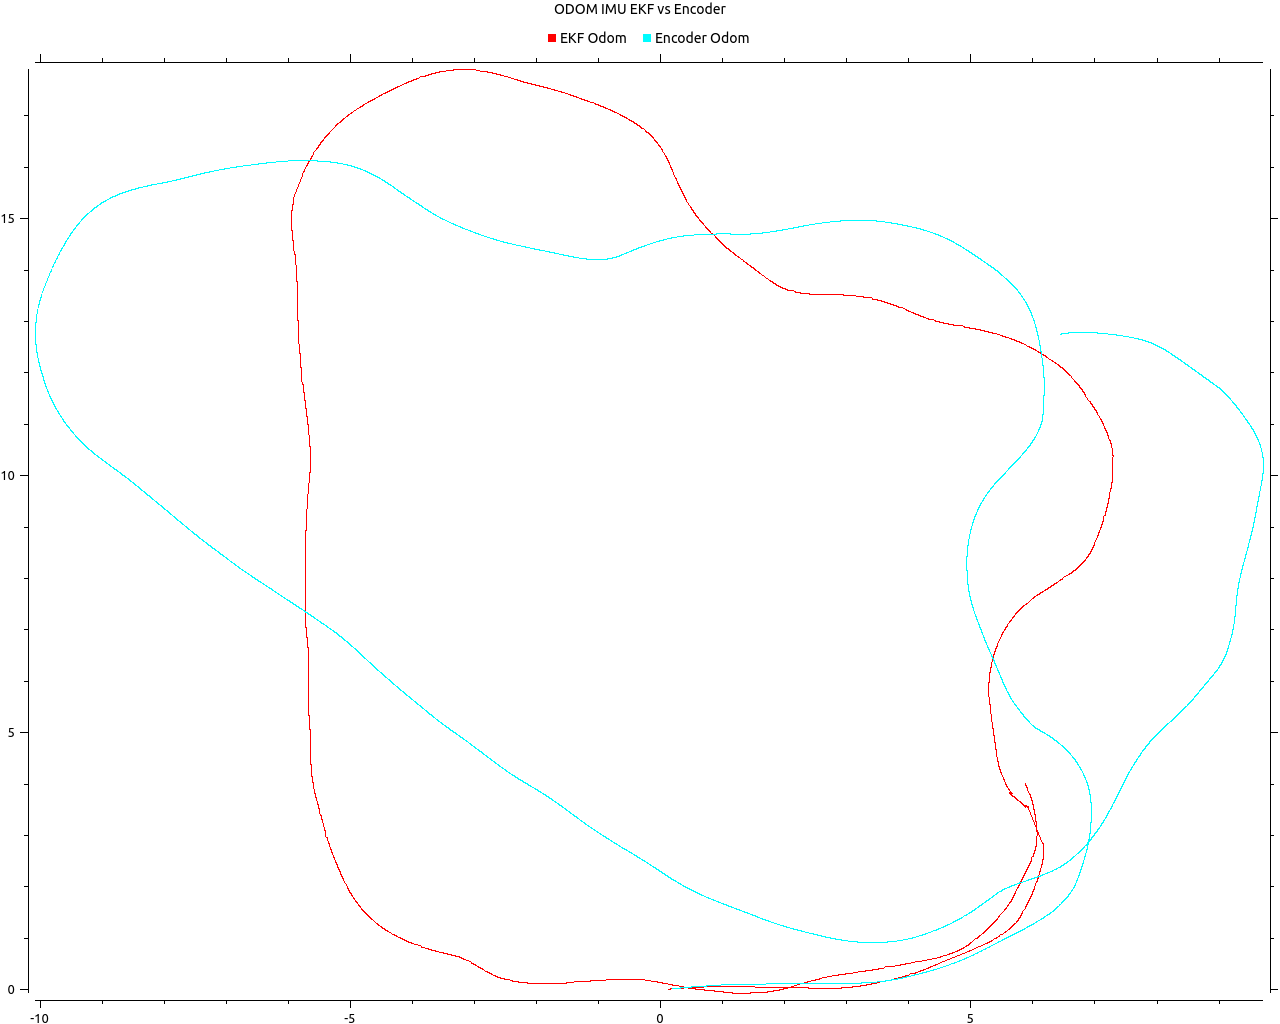
\includegraphics[width=\textwidth]{Pictures/odom after one round}
	\caption{Odometry comparison wheel odom + IMU + cmd\_vel}
	\label{Odometry comparison wheel odomIMUcmdvel}

\end{figure}
\begin{figure}[H]
	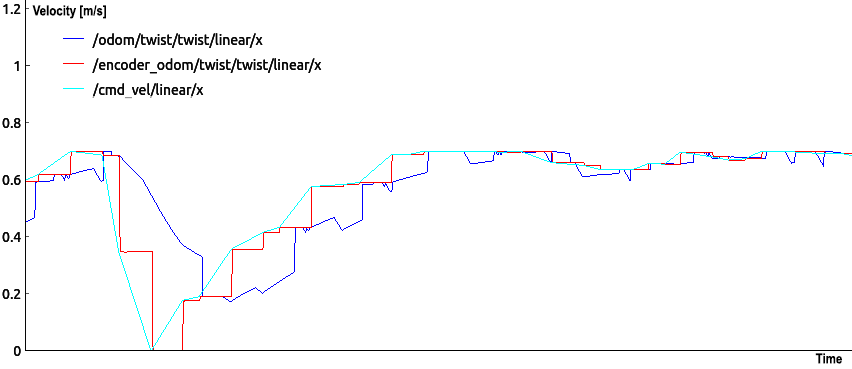
\includegraphics[width=\textwidth]{Pictures/circle vel}
	\caption{Velocity comparison with cmd\_vel}
	\label{velwithcmd}
\end{figure}



\begin{figure}[H]
	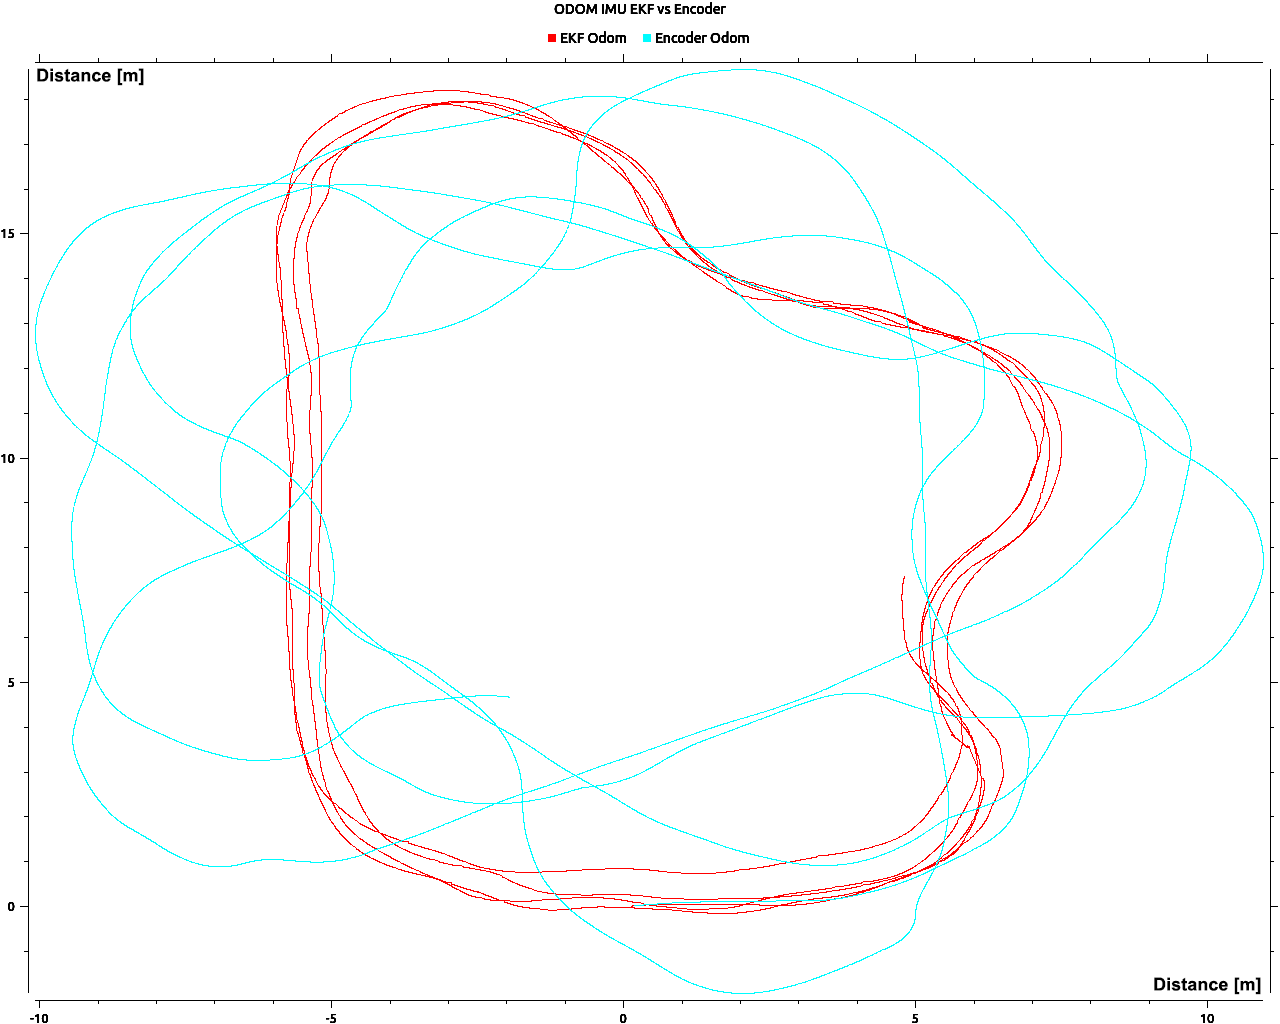
\includegraphics[width=\textwidth]{Pictures/odom comp multiple rounds}
	\caption{Odom comparison multiple rounds}
	\label{Odom comparison multiple rounds}

\end{figure}

Even after four rounds the odometry has not gained a large error in both translational and rotational as pictured in Figure \ref{Odom comparison multiple rounds}, furthermore the difference between the original odometry of the wheel encoders to the odometry from robot localization is quite remarkable.

After the rotantional and translational errors are marginal the scale of the odometry needs to be checked.
To isolate the different errors from the scaling error a circular track is build with a radius of 10 meter. Since the turning radius is constant this isolates the rotational error which can be seen at the graph of the wheel odometry in Figure \ref{circular track}.\\
The radius was chosen that high so potential errors are amplified and easier detectable.\\

Since the robot is driving on the lane and not on the middle road marking the expected radius is 10,45 meter. When evaluating the EKF odom in Figure \ref{circular track} we see that the scale is very precise.
 
\begin{figure}[H]
	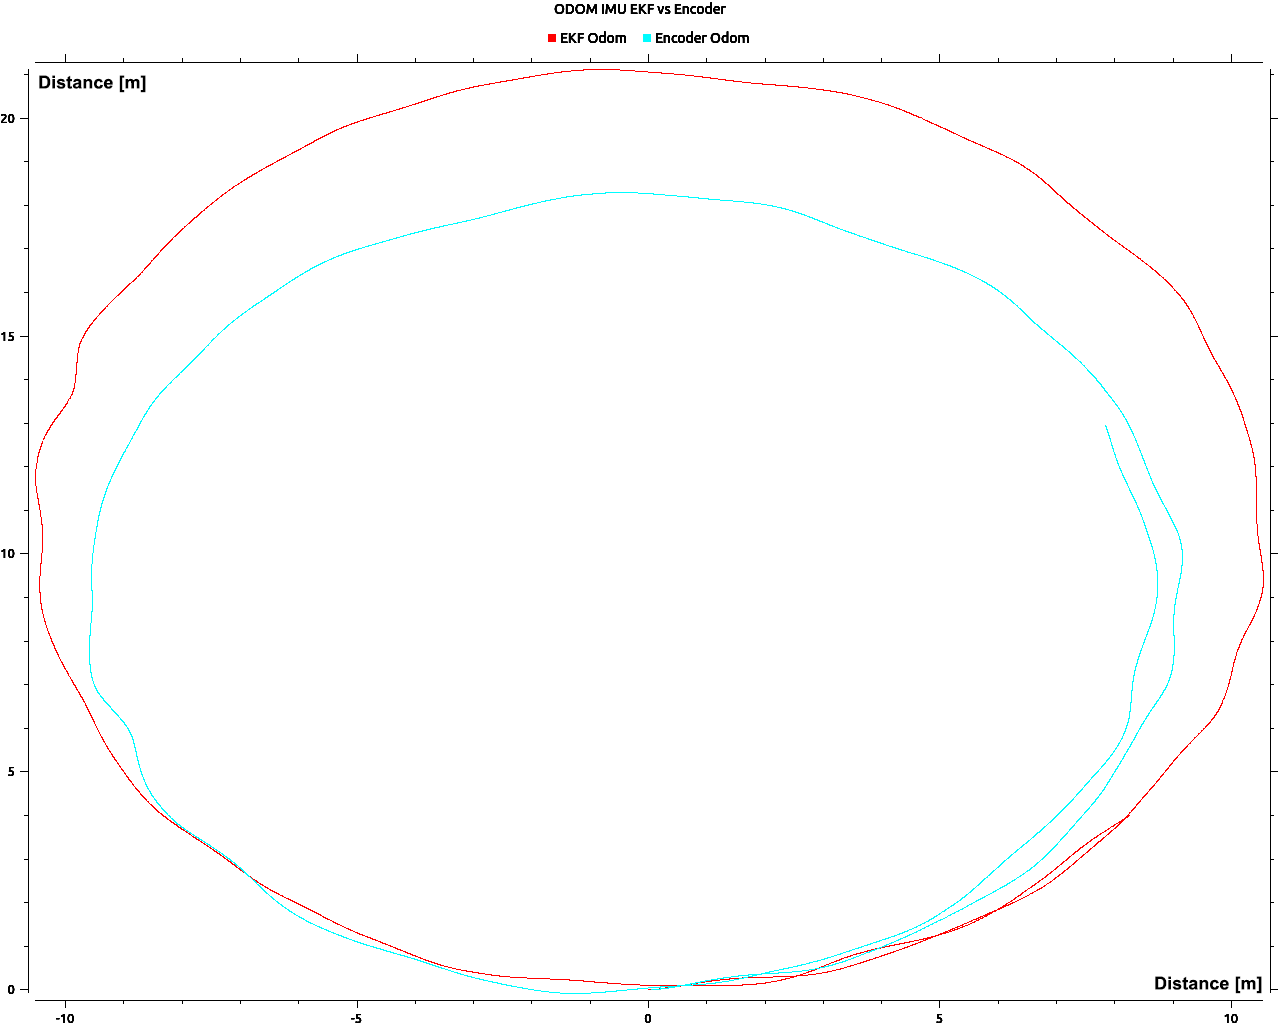
\includegraphics[width=\textwidth]{Pictures/circle odom}
	\caption{Odom comparison circular track}
	\label{circular track}

\end{figure}

As a final test the odometry from the robot\_localization node is compared to the true position from the simulation.

 \begin{figure}[H]
	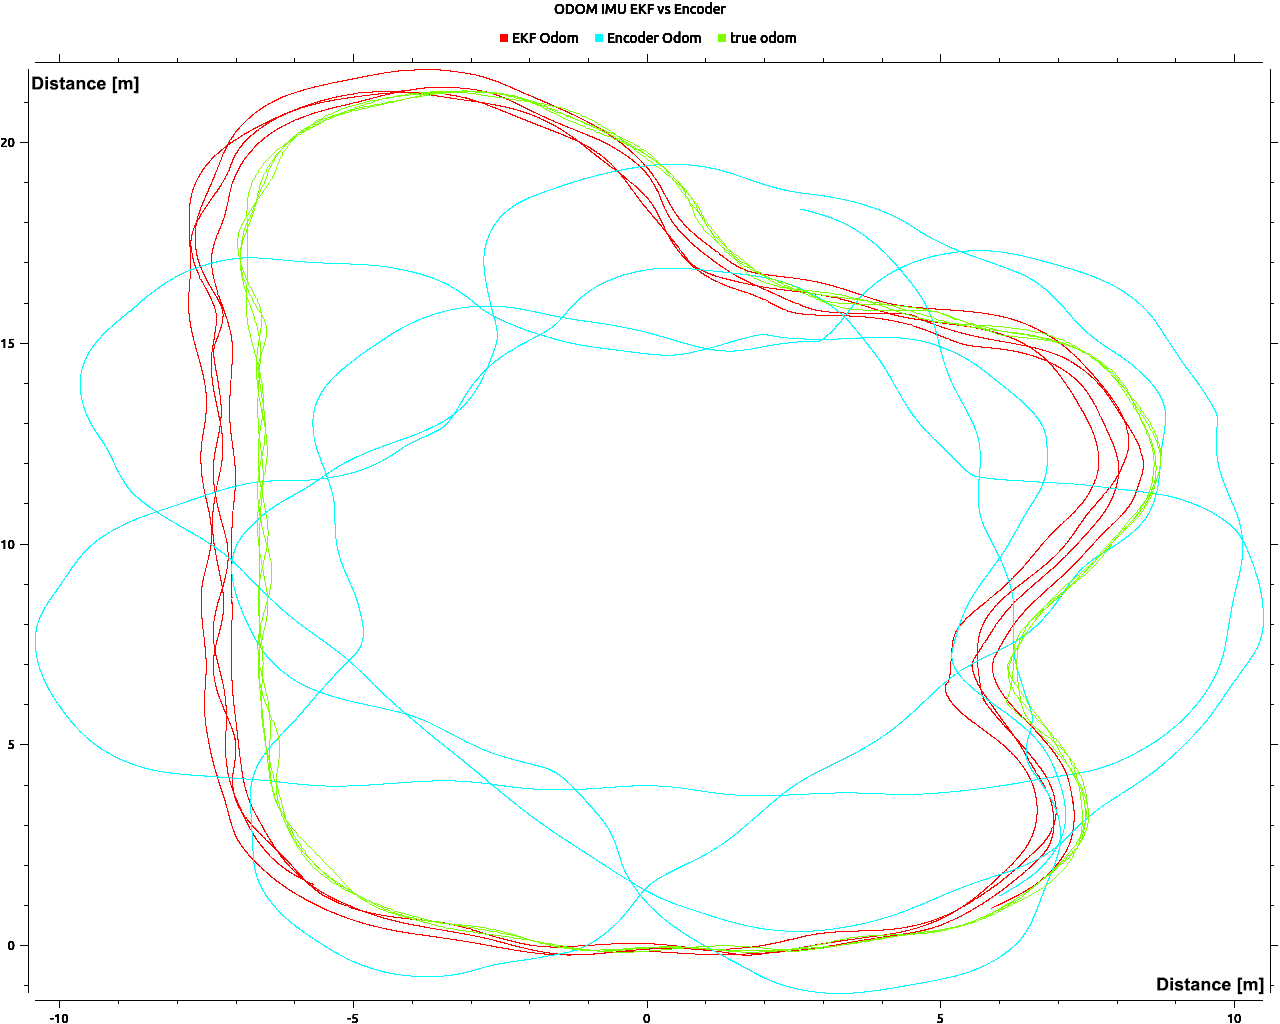
\includegraphics[width=\textwidth]{Pictures/odom with true}
	\caption{Comparison with true position}
	\label{trueodom}
\end{figure}

The comparison in Figure \ref{trueodom} shows, that the filtered odometry has a slight translational offset, but is very similar to the true odometry extracted from the simulation, hence it will be considered as sufficient for the navigation.


\section{Lidar test}


The Lidar sensor is simulated with realistic noise and errors. This also introduces the well known edge error in Laser distance measurement. 

When using a ``realistic'' lidar to project obstacles into the costmap this error produces a lot of lethal point like obstacles that significately hinder navigation as visible in Figure \ref{unfiltered lidar}.

\begin{figure}[H]
	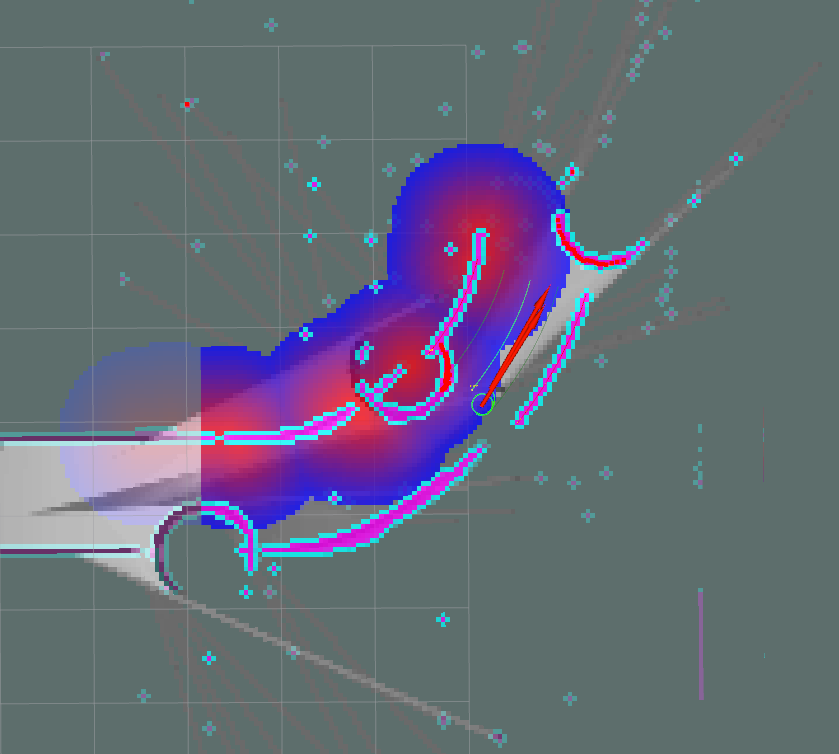
\includegraphics[width=\textwidth]{Pictures/Needs filtering of Laser}
	\caption{Lidar Test result}
	\label{unfiltered lidar}
\end{figure}

\subsection{Optimization}
To remove these error measurements the ROS package ``laser\_filters'' can be used. Among many different filter plugins that can be constructed into a filter chain it features the filter plugin ``ScanShadowFilter'' that is developed to remove the veiling effect around obstacles cause by the edge effect \cite{laserfilters}.


Figure \ref{lasercomp} shows a comparison between the filtered and not filtered laser scan, while keeping the data for 10 seconds. This allows to see the quickly jumping outliers caused by the edge effect. The filter seems well configured since the filtered points have no single outlier but still featuring a very good representation of the measured obstacle.

\begin{figure}[H]
	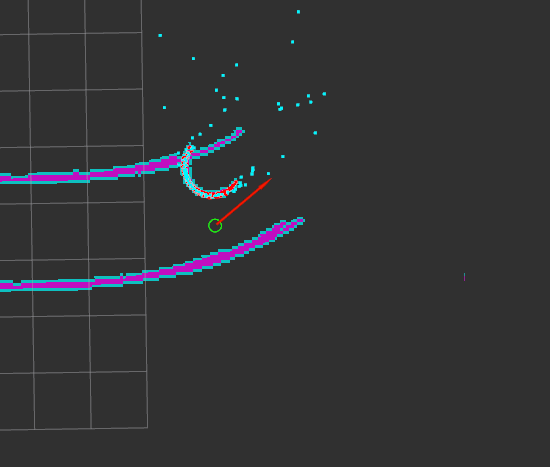
\includegraphics[width=\textwidth]{Pictures/LASERFILTER COMP}	
	\caption{comparison between filtered and not filtered laser scan (red - filtered, turquoise - raw)}
	\label{lasercomp}
\end{figure}

\section{road\_detection test}

As pictured in Figure \ref{longdurroad} the performance of the road detection converges to ca. 98.8\%. At the beginning the graph is not as reliable since there have not yet been enough measurements.\\

The duration of the test was roughly 1.5 hours of continuous navigation without obstacles in the simulation.

\begin{figure}[H]
	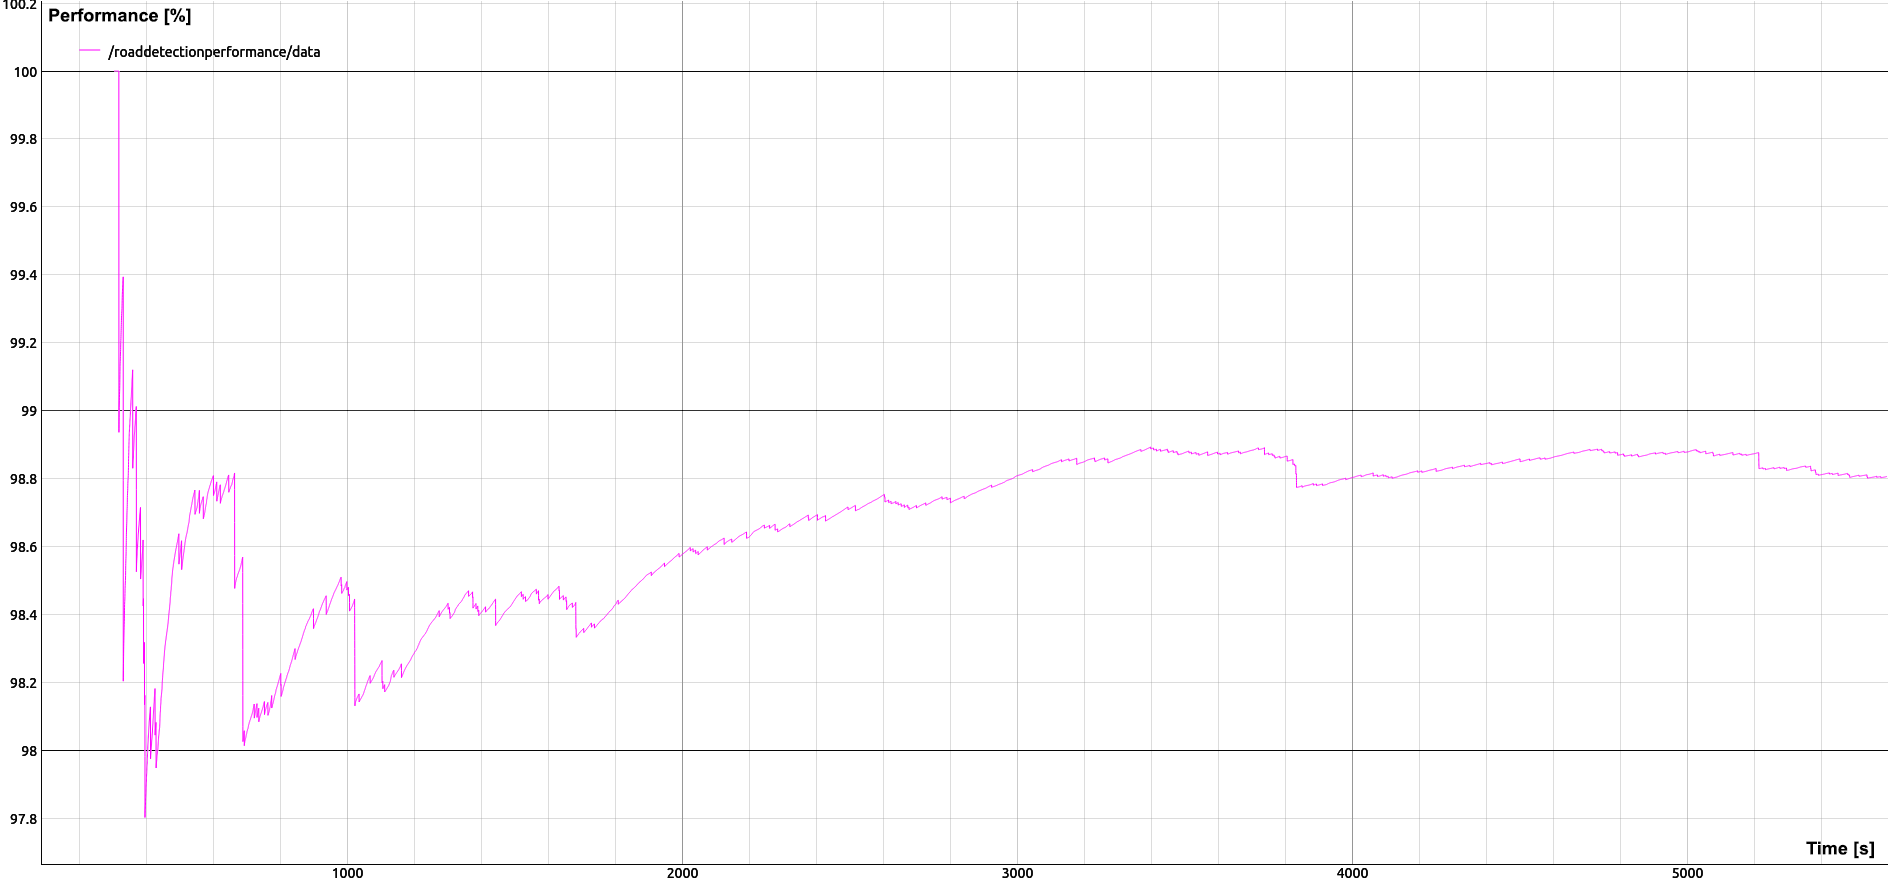
\includegraphics[width=\textwidth]{Pictures/long duration road detection test}
	\caption{roadRecordEvaluation during long duration test}
	\label{longdurroad}
\end{figure}

\section{SLAM test}
\textbf{Data purely from road detection:}\\

The following pictures contain the SLAM map after the \nth{1},\nth{2} and \nth{3} round.\\

\begin{figure}[H]
	\centering
	\begin{subfigure}{.3\linewidth}
		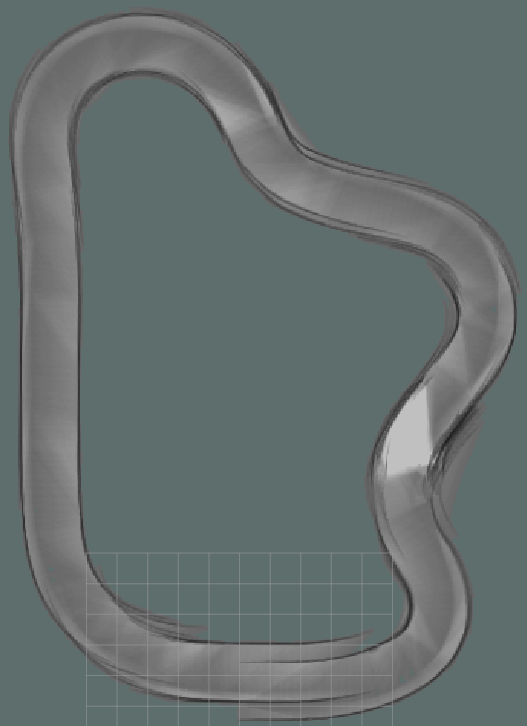
\includegraphics[width=\textwidth]{Pictures/1slamtest1}
		\caption{First}
		\end{subfigure}	
	%\hskip2em
	\begin{subfigure}{.3\linewidth}
		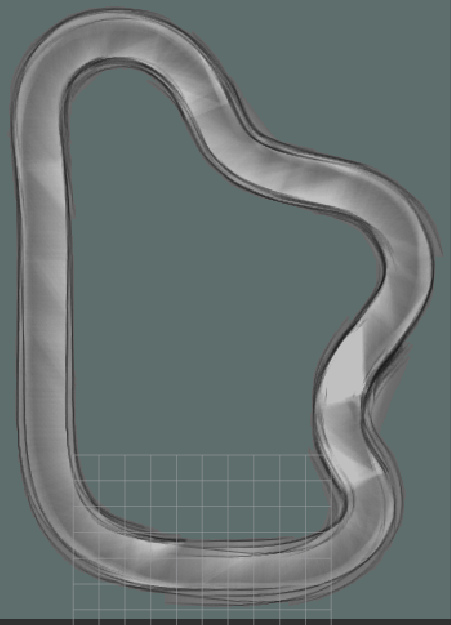
\includegraphics[width=\textwidth]{Pictures/1slamtest2}
		\caption{Second}
	\end{subfigure}
	%\hskip2em
	\begin{subfigure}{.3\linewidth}
		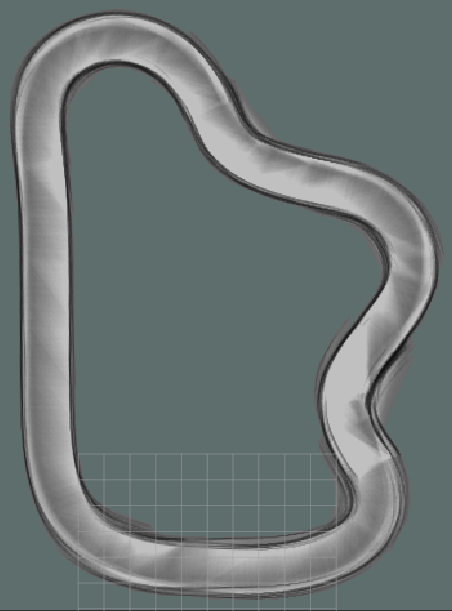
\includegraphics[width=\textwidth]{Pictures/1slamtest3}
		\caption{Third}
	\end{subfigure}

	\caption{Slam Map of first three rounds}
	\label{1slamtest}

\end{figure}

In the first round the map is not yet optimized. Like pictured in  Figure \ref{1slamtest} the road is not connected at the bottom after the first round, but has slight translational error.\\
In the second round the road is closed, but some submaps are slightly misaligned which can be seen by the blurry road markings.\\
This is well corrected in the third round and will improve from here on with every round, until the computational effort is too high.\\

\textbf{Data purely from localization and lidar scan with obstacles on the side of the road:}\\


As pictured in Figure \ref{2slamtest} cartographer manages to close the road already after the first round. After the second round the road borders are slightly blurry, therefore the submaps are not yet perfectly matched. This blurriness slightly improves after the third round, but the submaps are not yet perfectly matched with each other.

\begin{figure}[H]
	\centering
	\begin{subfigure}{.3\linewidth}
		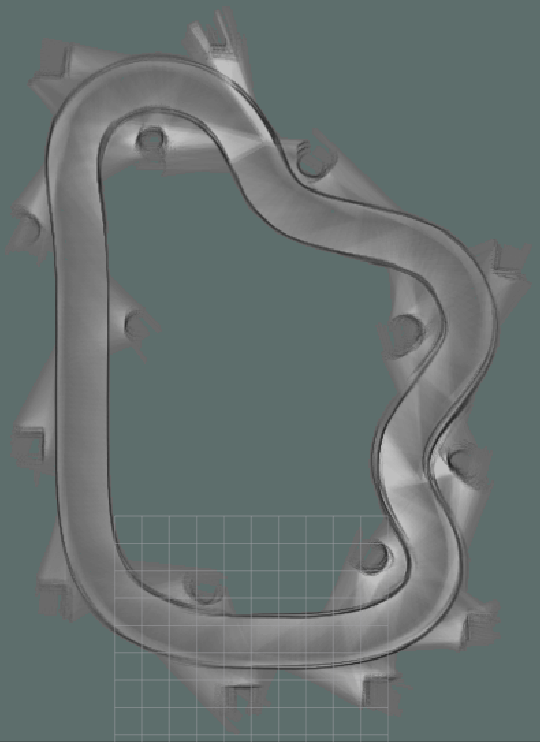
\includegraphics[width=\textwidth]{Pictures/2slamtest1}
		\caption{\nth{1} round}
		\end{subfigure}	
	%\hskip2em
	\begin{subfigure}{.3\linewidth}
		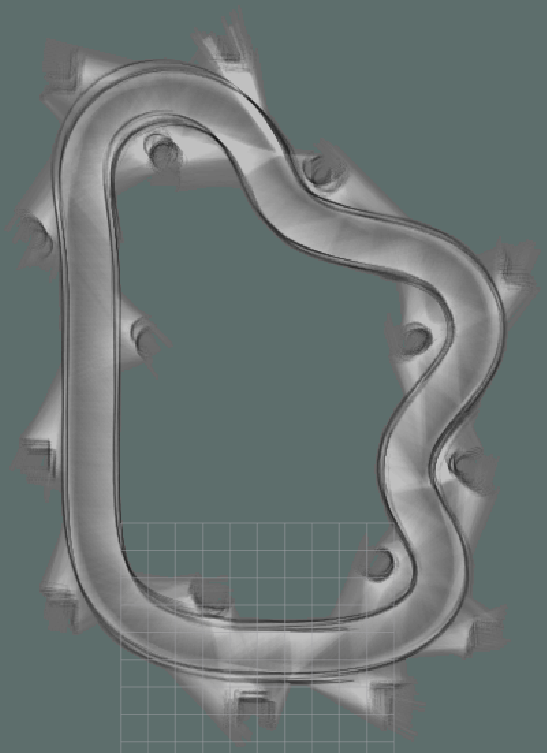
\includegraphics[width=\textwidth]{Pictures/2slamtest2}
		\caption{\nth{2} round}
	\end{subfigure}
	%\hskip2em
	\begin{subfigure}{.3\linewidth}
		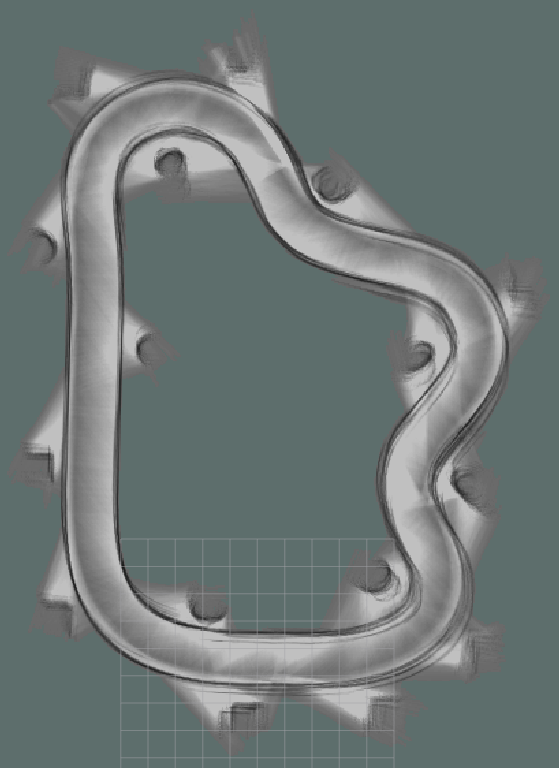
\includegraphics[width=\textwidth]{Pictures/2slamtest3}
		\caption{\nth{3} round}
	\end{subfigure}

	\caption{Slam Map of first three rounds}
	\label{2slamtest}

\end{figure}



\textbf{Long duration test with both road detection and lidar scan with obstacles on the side of the road:}\\

The map build by cartographer during this test (Figure \ref{3slamtest}) shows, that the map builds a very good representation of the real environment over the first four rounds.\\

After the \nth{7} round it is noticeable, that the matching of submaps seems to take more and more time, which is visible by a trace of unmatched submaps, that are slightly shifted. This is caused by the computational burden caused by the amount of submaps. In this round the cartographer node already takes up 20\% of the cpu resources and increases continuously. At this point realtime scan and submap matching is not possible anymore, resulting in enormous processing delays.

\begin{figure}[H]
	\centering
	\begin{subfigure}{.3\linewidth}
		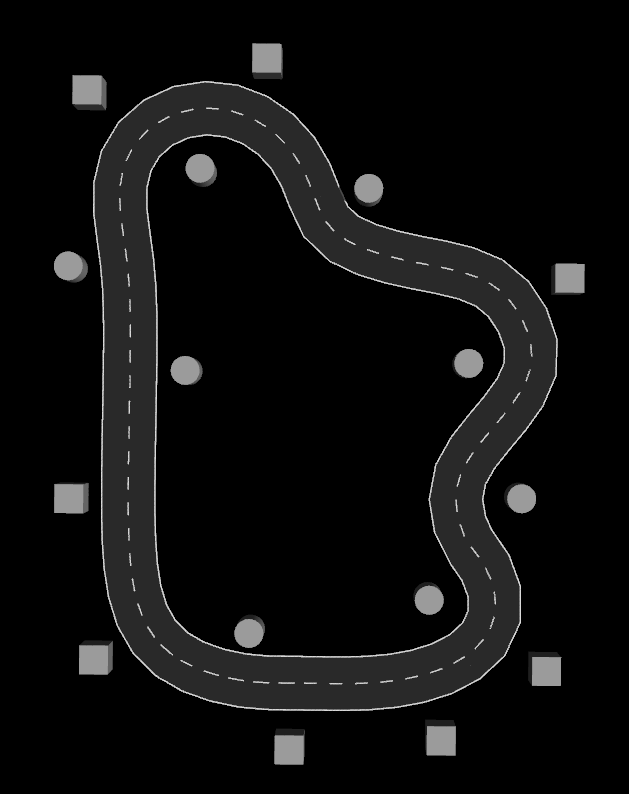
\includegraphics[width=\textwidth]{Pictures/2slamtest}
		\caption{Real Environment}
		\end{subfigure}	
	%\hskip2em
	\begin{subfigure}{.3\linewidth}
		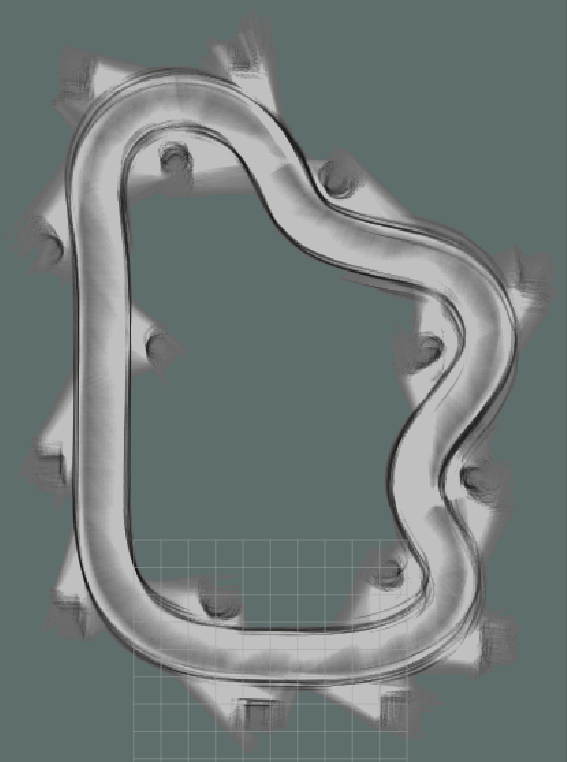
\includegraphics[width=\textwidth]{Pictures/2slamtest4}
		\caption{\nth{4} round}
	\end{subfigure}
	%\hskip2em
	\begin{subfigure}{.3\linewidth}
		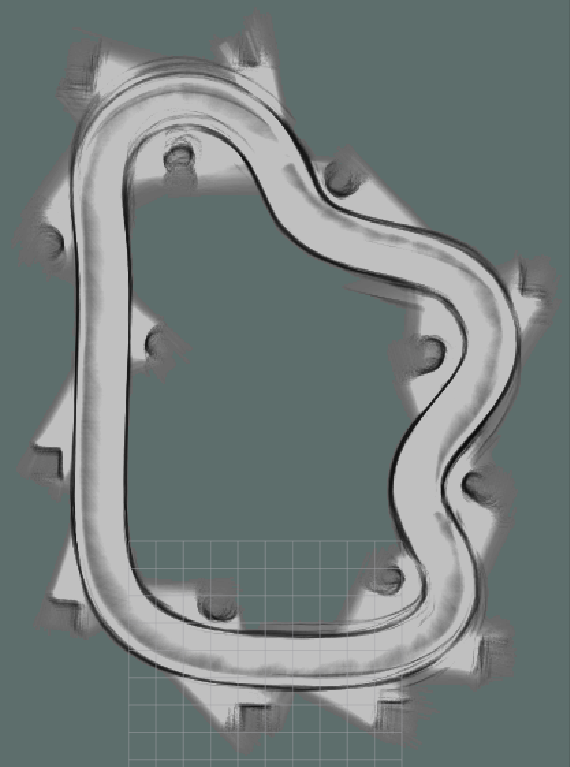
\includegraphics[width=\textwidth]{Pictures/2slamtest7}
		\caption{\nth{7} round}
	\end{subfigure}

	\caption{Slam Map rounds during long duration test}
	\label{3slamtest}

\end{figure}


\textbf{Data purely from localization and lidar scan with obstacles on the road:}\\

\begin{figure}[H]
	\centering
	\begin{subfigure}{.3\linewidth}
		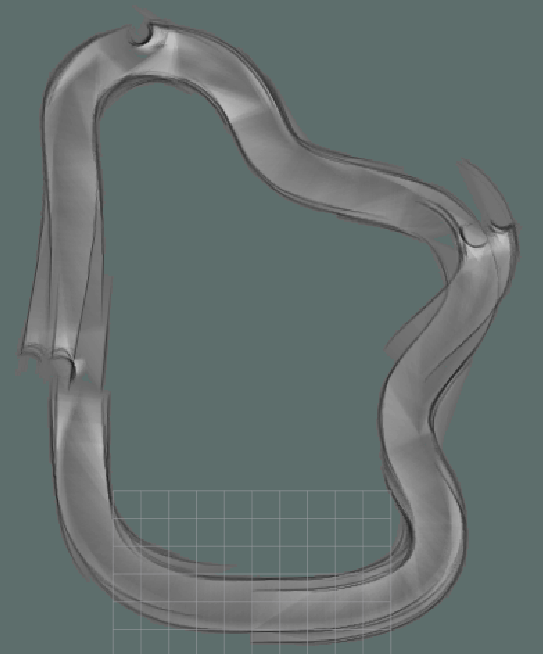
\includegraphics[width=\textwidth]{Pictures/3slamtest1}
		\caption{\nth{1} round}
		\end{subfigure}	
	%\hskip2em
	\begin{subfigure}{.3\linewidth}
		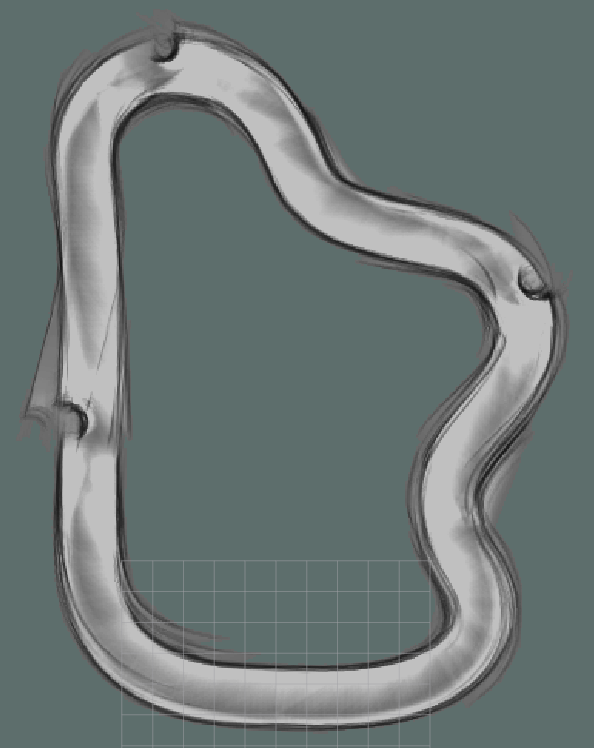
\includegraphics[width=\textwidth]{Pictures/3slamtest4}
		\caption{\nth{4} round}
	\end{subfigure}
	%\hskip2em
	\begin{subfigure}{.3\linewidth}
		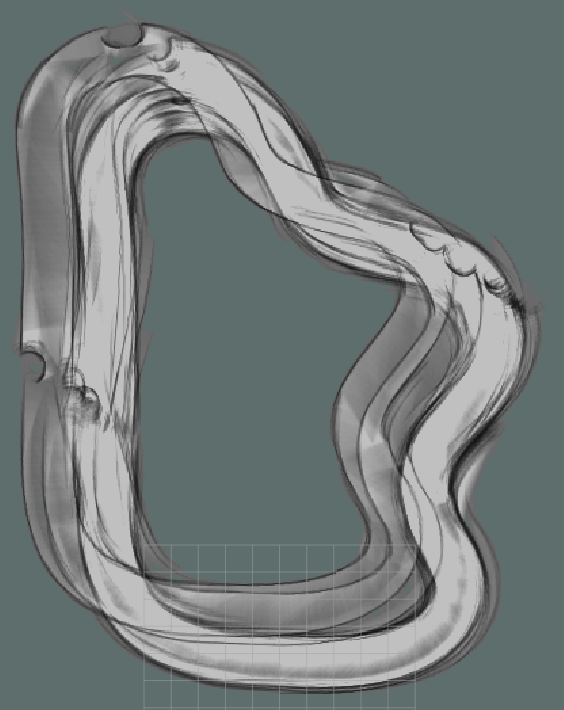
\includegraphics[width=\textwidth]{Pictures/3slamtest10}
		\caption{\nth{10} round}
	\end{subfigure}

	\caption{Slam Map rounds during long duration test}
	\label{4slamtest}

\end{figure}

As pictured in \ref{4slamtest} cartographer struggles with aligning the submaps during obstacle avoidance and suffers from rotational error.\\
Fortunately these errors are mostly corrected over the period of the next few rounds.\\ In the \nth{10} round however cartographer suffers from the same issue highlighted by the long duration test. Here it is clearly visible, that the queue of unmatched submaps is more than one entire round.\\

\textbf{Discussion of the test results}\\
As proven by the first two tests, cartographer is well tuned and the map would be useable for goal extraction. The submaps are well alligned and the map has no huge translational or rotational offset.\\

The \nth{3} and \nth{4} test on the other hand display the limitations of the slam algorithm in this use case.\\
When obstacles are located on the right lane the allignment of the submaps fails and a lot of submaps cant be attached to the rest of the map. After passing the same obstacle in multiple rounds the map improves to a point where it would be usable for goal extraction.\\
The \nth{3} test proves that cartographer is not usable in SLAM mode during long time navigation an a circuit. This is caused by the amount of submaps that are close to each other and the resulting amount of constraints between each of them.

Based on these test results it is not feasible to use the SLAM map for navigation with obstacles on the road, since the map is just not reliable enough and it is not certain of there are obstacles on the road or not. 




\section{complete system test}
The following subsections cover the discussion of the complete system tests.
\textbf{No obstacles}\\
The reasoning for this test is, to check how good the robot stays on the right lane. Therefore the robot drives in the described test environment, while the difference between the right lane and the robot center is monitored.

\begin{figure}[H]
	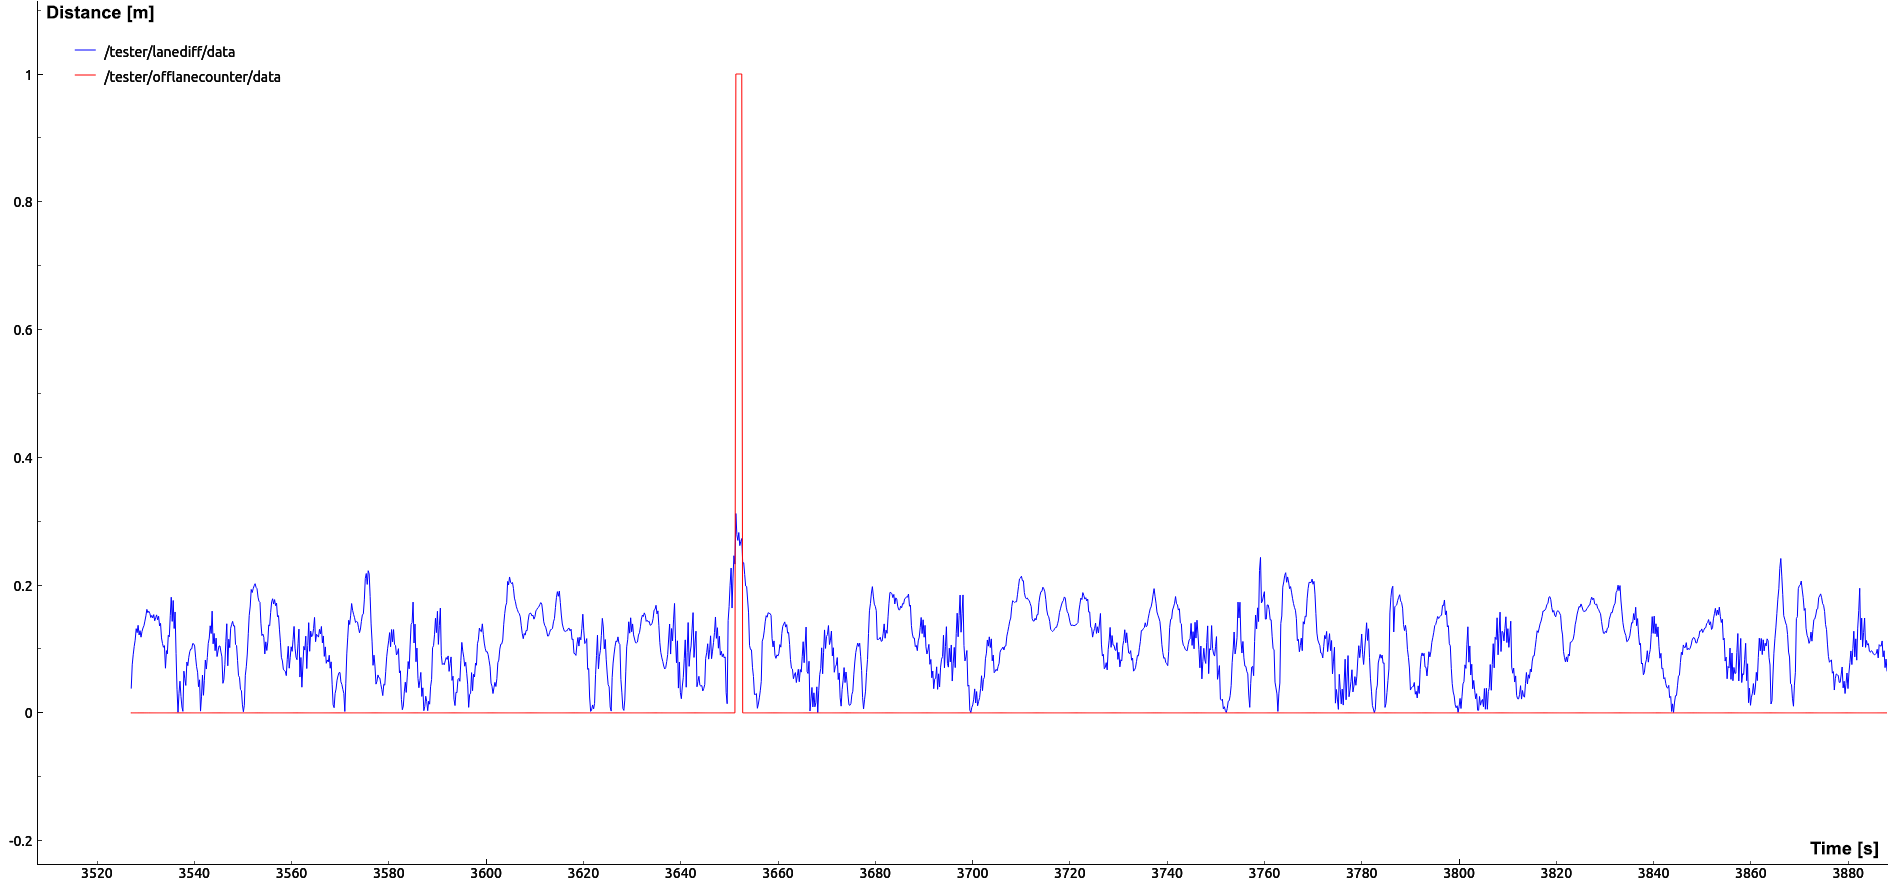
\includegraphics[width=\textwidth]{Pictures/final analysis no obstacle}
	\caption{absolute error of the robot trajectory and rectified signal of the avoidance duration}
	\label{noobserr}
\end{figure}

As pictured in \ref{noobserr} the robot has left the road markings once.\\

\begin{figure}[H]
	\begin{subfigure}{.5\linewidth}
		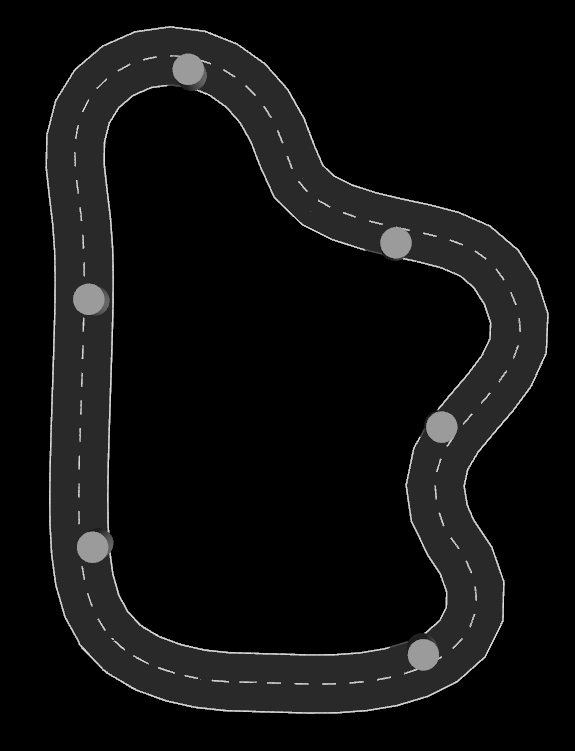
\includegraphics[width=\textwidth]{Pictures/obstacle left final 2}
		\caption{obstacles on left lane}
	\end{subfigure}	
	%\hskip2em
	\begin{subfigure}{.5\linewidth}
		\includegraphics[width=\textwidth]{Pictures/right final obs}
		\caption{obstacles on right lane}
	\end{subfigure}

	\caption{Obstacle placement for both final tests}
	\label{obstaclefinaltest}

\end{figure}
\textbf{Obstacles on left lane}\\
This test is supposed to test the behavior of the navigation when obstacles block the view of the camera but the robot has to drive on the right side. In this test the robot will not drive as many rounds, since the goal is to observe the behavior when passing goals. In contrast to Figure \ref{noobserr} the distance to the nearest obstacle will be included in the graph, thus it can be determined, if the robot left the lane because it is near an obstacle or not, for this the true positions from the simulation will be used. The obstacle distance will only be tracked, if it is below 3 meters.
\begin{figure}[H]
	\includegraphics[width=\textwidth]{Pictures/left obs final obs2}
	\caption{graph of left lane obstacle test}
	\label{leftobsfinal}
\end{figure}
As visible in figure \ref{leftobsfinal} the robot left the right lane way more often compared to \ref{noobserr}.\\

\textbf{Obstacles on right lane}\\

To cover the possible scenarios of the carolo cup this test is supposed to be a realistic application with a few obstacle scattered over the entire environment on the right lane. Like in the last test the obstacles will be located as well in corners, as on straight sections of the road.

\begin{figure}[H]
	\includegraphics[width=\textwidth]{Pictures/right obs final obs}
	\caption{graph of right lane obstacle test}
	\label{rightobsfinal}
\end{figure}


As pictured in Figure \ref{obstaclefinaltest}, there are five obstacles on the right lane. These can be seen, when inspecting the graphe in Figure \ref{rightobsfinal}, which shows two rounds of the robot.

Furthermore the graph shows, that the robot successfully avoided all obstacles in both rounds. Unfortunately the robot left the lane three times, when no obstacle in the proximity of it.\\

In the middle of the graph the robot took particularly long for the avoidance.

The graph also shows, that the avoidance is all ways finished before the robot is two meters away from the obstacle and therefore satisfies this condition.

\subsection{Discussion}

The results of the complete system tests show, that the navigation performs really well during simple lane following, since the road detection recognizes the road almost allways as shown in the road\_detection test.

While observing the robot during driving past obstacles on the left lane it was noticeable, that the robot mostly left the lane, directly after it passed an obstacle in or directly after a corner.\\ 
In this case the predicted goal pulls the robot into the middle of the road, since the costmap does not yet have information about the road and therefore will not force the global plan to the right lane. The approximated goal is still constructed with the circle approximation since the upcoming straight section has net yet been seen.\\

Obstacle avoidance suffers from a similar problem. As shown in the \nth{3} test. Here it is visible, that the robot passes the obstacle nicely, but after passing drives along the center of the road, which causes the spikes of the rectified signal visible in \ref{rightobsfinal} after the ovoidance. As soon as the robot has passed an obstacle fully it drives straight to the predicted goal while waiting on new data from the road\_detection, which often causes unnecessary long avoidance periods.







\chapter{Conclusion}
\label{Conclusion}
The goal of this thesis was the configuration and development of a software stack that allows a mobile platform to drive autonomously in a road like environment, while avoiding obstacles and preferring the right lane.
This has been achieved by formulating a concept and implementing it using the navigation stack of ROS and various open source plugins and packages.
For the remaining tasks packages containing nodes have been developed using C++ which are configurable for different environments and robots. These packages are provided in a git repository hosted at the following url.\\

\url{https://github.com/Tristan9497/RoutePlanning}\\

The resulting navigation has been tested in a simulated environment as a complete stack, aswell as the individual nodes them selves.\\

Testing allowed to highlight the strengths and weaknesses of the concept, which can be used as the guideline for future work on the established structure. The developed concept was found to be working good, especially on empty road sections.\\

With an increasing amount of obstacles the amount of times where the camera sees the road markings decreases, which therefore causes the navigation to fail.


\section{Personal conclusion}







\chapter{Outlook}
\label{outlook}

This thesis highlighted existing problems in the established navigation concept, which should be resolved to score high results in the Carolo-Cup. This section will give proposals and ideas for future work on the current state of the navigation.\\

Using the structure of move\_base a custom local and global planner plugin can be developed and exchanged with the current plugins.\\

It could be very interesting to explore different path finding algorithms than the ones offered in the global\_planner plugin. At this point the development of a custom global planner might be able to perform better given the known use case.\\

Seeing the performance of the elastic band in the local planner used in this thesis a potential approach could be to move the task of lane following to the local planner, by deforming the elastic band directly with the polynomials of the road detection and weighting them individually.\\

To decrease the amount of times, where the navigation has to wait until it receives data from the road\_detection, the approximated shape of the road could be drawn into the costmap and overwritten by new incoming data of the road. This could be implemented into the dynamic\_cost\_layer that has been developed during this work.

The exploration of V-REP or its successor CoppeliaSim might be interesting with focus on the sensor plugins, especially with focus on distortion of the camera image.\\

During the research required in this work Nav2 for ROS2, which is currently in development seemed to offer many features, that are not included in the current navigation stack of ROS Noetic. As this thesis is focused on the development based on ROS Noetic this has not been explored yet. Nav2 features a new implementation of a costmap, that features filters usable to define keep-out or slow areas, that might be usable for a cleaner way to guide the robot on the right lane. Therefore further exploration of this might be beneficial.\\

As lidar based SLAM seemed to perform not ideal visual SLAM might offer more precision since the road markings might offer more informations for scan matching than the extracted polynomials. Furthermore functionality to detect, if a map is closed and of a reasonable quality might be usable to end the SLAM procedure, export the current map and using localization only to avoid the problem of the steadily increasing computational burden.


\listoffigures %Abbildungsverzeichnis

\listoftables %Tabellenverzeichnis

%\lstlistoflistings %Quelltextverzeichnis

%\printnomenclature %Abküzungsverzeichnis

\renewcommand{\bibname}{References}
\printbibliography


%ANHANG
\cleardoublepage
\pagenumbering{Roman} %Big romanian Pagenumbering
\setcounter{page}{1} %Seitenzähler zurücksetzen

\thispagestyle{plain}
\appendix %Anhang einfuegen


%TABLE OF CONTENTS APPENDIX
\phantomsection
\addcontentsline{toc}{chapter}{Appendix}
\startcontents[appendix]
\renewcommand\contentsname{\huge Appendix}% if a change of the default "Contents" name is required
\printcontents[appendix]{ }{0}{\section*{\contentsname}}
\stopcontents[main]
\newpage
%APPENDIX
\chapter{Source Code}
\label{appendixSoureCode}




\chapter{Additional Topics}
\label{AppendixAdditionalTopics}














\stopcontents[appendix]

\begin{otherlanguage}{ngerman}
\addchap*{Eidesstattliche Erklärung}

\vspace*{5mm}

\thispagestyle{empty}

\begin{flushleft}
\begin{tabular}[h]{p{60mm}l p{60mm}l}
\textbf{Name:} Schwörer 			&\textbf{Vorname:} Tristan\\
\textbf{Matrikel-Nr.:} 71336		&\textbf{Studiengang:} Mechatronik\\
\end{tabular}
\end{flushleft}

\vspace*{11mm}

Hiermit versichere ich, \textbf{Tristan Schwörer}, an Eides statt, dass ich die vorliegende Bachelorarbeit

an der \textbf{Hochschule Aalen}

mit dem Titel \textbf{„Entwicklung von Navigationssoftware für mobile Robotersysteme und Simulation“}

selbständig und ohne fremde Hilfe verfasst und keine anderen als die angegebenen Hilfsmittel benutzt habe. Die Stellen der Arbeit, die dem Wortlaut oder dem Sinne nach anderen Werken entnommen wurden, sind in jedem Fall unter Angabe der Quelle kenntlich gemacht.\\

Ich habe die Bedeutung der eidesstattlichen Versicherung und prüfungsrechtlichen Folgen (\S 23 Abs. 3 des allg. Teils der Bachelor-SPO der Hochschule Aalen) sowie die strafrechtlichen Folgen (siehe unten) einer unrichtigen oder unvollständigen eidesstattlichen Versicherung zur Kenntnis genommen.\\

\vspace*{5mm}
\Large\textbf{Auszug aus dem Strafgesetzbuch (StGB)}


\normalsize\textbf{\S 156 StGB} Falsche Versicherung an Eides Statt

Wer von einer zur Abnahme einer Versicherung an Eides Statt zuständigen Behörde eine solche Versicherung falsch abgibt oder unter Berufung auf eine solche Versicherung falsch aussagt, wird mit Freiheitsstrafe bis zu drei Jahren oder mit Geldstrafe bestraft.

\vspace*{20mm}


\rule[-0.2cm]{5cm}{0.5pt} \hspace*{30mm}\rule[-0.2cm]{5cm}{0.5pt}
\newline
Ort, Datum\hspace*{61.85mm}Unterschrift

\end{otherlanguage} 


\end{document}
%%%%%%%%%%%%%%%%%%%%%%%%%%%%%%%%%%%%%%%%%%%%%%%%%%%%%%%%%%%%
%END_OF_FILE

















